% Options for packages loaded elsewhere
\PassOptionsToPackage{unicode}{hyperref}
\PassOptionsToPackage{hyphens}{url}
%
\documentclass[
]{article}
\usepackage{lmodern}
\usepackage{amssymb,amsmath}
\usepackage{ifxetex,ifluatex}
\ifnum 0\ifxetex 1\fi\ifluatex 1\fi=0 % if pdftex
  \usepackage[T1]{fontenc}
  \usepackage[utf8]{inputenc}
  \usepackage{textcomp} % provide euro and other symbols
\else % if luatex or xetex
  \usepackage{unicode-math}
  \defaultfontfeatures{Scale=MatchLowercase}
  \defaultfontfeatures[\rmfamily]{Ligatures=TeX,Scale=1}
\fi
% Use upquote if available, for straight quotes in verbatim environments
\IfFileExists{upquote.sty}{\usepackage{upquote}}{}
\IfFileExists{microtype.sty}{% use microtype if available
  \usepackage[]{microtype}
  \UseMicrotypeSet[protrusion]{basicmath} % disable protrusion for tt fonts
}{}
\makeatletter
\@ifundefined{KOMAClassName}{% if non-KOMA class
  \IfFileExists{parskip.sty}{%
    \usepackage{parskip}
  }{% else
    \setlength{\parindent}{0pt}
    \setlength{\parskip}{6pt plus 2pt minus 1pt}}
}{% if KOMA class
  \KOMAoptions{parskip=half}}
\makeatother
\usepackage{xcolor}
\IfFileExists{xurl.sty}{\usepackage{xurl}}{} % add URL line breaks if available
\IfFileExists{bookmark.sty}{\usepackage{bookmark}}{\usepackage{hyperref}}
\hypersetup{
  pdftitle={Especificación de requisitos},
  hidelinks,
  pdfcreator={LaTeX via pandoc}}
\urlstyle{same} % disable monospaced font for URLs
\usepackage{longtable,booktabs}
% Correct order of tables after \paragraph or \subparagraph
\usepackage{etoolbox}
\makeatletter
\patchcmd\longtable{\par}{\if@noskipsec\mbox{}\fi\par}{}{}
\makeatother
% Allow footnotes in longtable head/foot
\IfFileExists{footnotehyper.sty}{\usepackage{footnotehyper}}{\usepackage{footnote}}
\makesavenoteenv{longtable}
\usepackage{graphicx}
\makeatletter
\def\maxwidth{\ifdim\Gin@nat@width>\linewidth\linewidth\else\Gin@nat@width\fi}
\def\maxheight{\ifdim\Gin@nat@height>\textheight\textheight\else\Gin@nat@height\fi}
\makeatother
% Scale images if necessary, so that they will not overflow the page
% margins by default, and it is still possible to overwrite the defaults
% using explicit options in \includegraphics[width, height, ...]{}
\setkeys{Gin}{width=\maxwidth,height=\maxheight,keepaspectratio}
% Set default figure placement to htbp
\makeatletter
\def\fps@figure{htbp}
\makeatother
\setlength{\emergencystretch}{3em} % prevent overfull lines
\providecommand{\tightlist}{%
  \setlength{\itemsep}{0pt}\setlength{\parskip}{0pt}}
\setcounter{secnumdepth}{-\maxdimen} % remove section numbering

\title{Especificación de requisitos}
\author{}
\date{}

\begin{document}
\maketitle

\hypertarget{introducciuxf3n}{%
\section{Introducción}\label{introducciuxf3n}}

En este anexo se especifican todos los requisitos funcionales y no
funcionales de la aplicación \emph{software} propuesta, incluyendo todos
aquellos que han sido aportados por complementos (\emph{plugins}).

La aplicación se divide en dos áreas bien diferenciadas, una pública
(\emph{frontend}) y otra de administración (\emph{backend}). Por este
motivo, se llevará a cabo una especificación de requisitos para cada
área.

\hypertarget{objetivos-generales}{%
\section{Objetivos generales}\label{objetivos-generales}}

Los objetivos generales que se desean alcanzar con el desarrollo del
proyecto son los siguientes:

\begin{itemize}
\item
  Proporcionar una infraestructura \emph{software} que permita:

  \begin{quote}
  \begin{itemize}
  \tightlist
  \item
    Gestionar los (meta)datos del CENIEH en la integración con
    ARIADNEplus.
  \item
    Transformar el esquema de (meta)datos de origen (CENIEH) a un
    esquema estandarizado compatible con ARIADNEplus.
  \item
    Compartir los datos de forma que estos sean accesibles desde el
    exterior.
  \item
    Facilitar la integración de los (meta)datos en ARIADNEplus.
  \end{itemize}
  \end{quote}
\end{itemize}

\hypertarget{catuxe1logo-de-requisitos}{%
\section{Catálogo de requisitos}\label{catuxe1logo-de-requisitos}}

En este apartado se muestran todos los requisitos considerados para
alcanzar todos y cada uno de los objetivos generales del proyecto.

\hypertarget{requisitos-funcionales-del-uxe1rea-puxfablica}{%
\subsection{Requisitos funcionales del área
pública}\label{requisitos-funcionales-del-uxe1rea-puxfablica}}

\begin{itemize}
\item
  \textbf{RFAP-1 Búsqueda de ítems públicos}: el usuario debe ser capaz
  de hacer una búsqueda sobre los ítems públicos almacenados en la
  plataforma.
\item
  \textbf{RFAP-2 Visualización de un ítem público}: el usuario debe
  poder visualizar el contenido (metadatos, tags, localización y/o
  ficheros) de un determinado ítem público.

  \begin{quote}
  \begin{itemize}
  \tightlist
  \item
    \textbf{RFAP-2.1 Ver fichero}: el usuario debe poder visualizar la
    información del fichero asociado a un determinado ítem público.
  \end{itemize}
  \end{quote}
\item
  \textbf{RFAP-3 Listado de ítems públicos}: el usuario debe poder
  listar todos los ítems públicos de la plataforma.
\item
  \textbf{RFAP-4 Listado de colecciones públicas}: el usuario debe poder
  listar todas las colecciones públicas almacenadas en la plataforma.
\item
  \textbf{RFAP-5 Visualización de una colección pública}: el usuario
  debe poder visualizar una colección pública.
\item
  \textbf{RFAP-6 Listado de etiquetas públicas}: el usuario debe poder
  listar todas las etiquetas existentes en la plataforma.
\item
  \textbf{RFAP-7 Búsqueda de ítems por localización}: el usuario debe
  poder buscar un ítem tomando como referencia su ubicación.
\item
  \textbf{RFAP-8 Información del proyecto}: el usuario debe poder
  conocer más información acerca del proyecto.
\end{itemize}

\hypertarget{requisitos-no-funcionales-del-uxe1rea-puxfablica}{%
\subsection{Requisitos no funcionales del área
pública}\label{requisitos-no-funcionales-del-uxe1rea-puxfablica}}

\begin{itemize}
\tightlist
\item
  \textbf{RNFAP-1 Usabilidad}: la aplicación debe presentar los datos de
  la forma más sencilla posible, evitando así que el usuario se pierda
  en el proceso de búsqueda o visualización.
\item
  \textbf{RNFAP-2 Internacionalización}: la aplicación debe contar con
  un sistema que permita mostrar el contenido de la interfaz en
  múltiples idiomas.
\item
  \textbf{RNFAP-3 Integridad}: la aplicación debe mostrar los datos tal
  y como se publicaron desde el área de administración, sin ningún tipo
  de alteración.
\end{itemize}

\hypertarget{requisitos-funcionales-del-uxe1rea-de-administraciuxf3n}{%
\subsection{Requisitos funcionales del área de
administración}\label{requisitos-funcionales-del-uxe1rea-de-administraciuxf3n}}

\begin{itemize}
\item
  \textbf{RFAA-1 Acceso al área de administración}: la aplicación debe
  controlar el acceso al área de administración.
\item
  \textbf{RFAA-2 Gestión de ítems}: la aplicación tiene que ser capaz de
  gestionar ítems.

  \begin{quote}
  \begin{itemize}
  \item
    \textbf{RFAA-2.1 Añadir ítem}: el operario debe poder añadir un
    nuevo ítem compuesto por metadatos, ficheros, etiquetas y una
    localización. Además, podrá asociarse a una colección, ser público o
    privado y ser destacado o normal.
  \item
    \textbf{RFAA-2.2 Editar ítem}: el operario debe poder editar el
    contenido de un ítem ya existente.
  \item
    \textbf{RFAA-2.3 Eliminar ítem}: el operario debe poder eliminar un
    ítem ya existente.
  \item
    \textbf{RFAA-2.4 Listar ítems}: el operario debe poder listar todos
    los ítems existentes.
  \item
    \textbf{RFAA-2.5 Ver ítem}: el operario debe poder visualizar todo
    el contenido asociado a un ítem.

    \begin{quote}
    \begin{itemize}
    \tightlist
    \item
      \textbf{RFAA-2.5.1 Exportar ítem}: el operario debe poder exportar
      un ítem ya existente.
    \end{itemize}
    \end{quote}
  \item
    \textbf{RFAA-2.6 Buscar ítems}: el operario debe poder buscar un
    ítem de entre todos los existentes.
  \item
    \textbf{RFAA-2.7 Exportar ítems}: el operario debe poder exportar
    varios ítems existentes a la vez.
  \end{itemize}
  \end{quote}
\item
  \textbf{RFAA-3 Gestión de colecciones}: la aplicación tiene que ser
  capaz de gestionar colecciones de ítems.

  \begin{quote}
  \begin{itemize}
  \item
    \textbf{RFAA-3.1 Añadir colección}: el operario debe poder añadir
    una colección nueva compuesta por metadatos o ficheros. Además,
    podrá ser pública o privada y ser destacada o normal.
  \item
    \textbf{RFAA-3.2 Editar colección}: el operario debe poder editar el
    contenido de una colección ya existente.

    \begin{quote}
    \begin{itemize}
    \tightlist
    \item
      \textbf{RFAA-3.2.1 Eliminar colección}: el operario debe poder
      eliminar una colección ya existente.
    \end{itemize}
    \end{quote}
  \item
    \textbf{RFAA-3.3 Listar colecciones}: el operario debe poder listar
    todas las colecciones existentes.
  \item
    \textbf{RFAA-3.4 Ver colección}: el operario debe poder visualizar
    toda la información relativa a una colección.

    \begin{quote}
    \begin{itemize}
    \tightlist
    \item
      \textbf{RFAA-3.4.1 Exportar colección}: el operario debe poder
      exportar una colección ya existente.
    \end{itemize}
    \end{quote}
  \end{itemize}
  \end{quote}
\item
  \textbf{RFAA-4 Gestión de tipos de ítem}: la aplicación tiene que ser
  capaz de gestionar tipos de ítem.

  \begin{quote}
  \begin{itemize}
  \item
    \textbf{RFAA-4.1 Añadir tipo de ítem}: el operario debe poder añadir
    un tipo de ítem con los elementps apropiados.
  \item
    \textbf{RFAA-4.2 Editar tipo de ítem}: el operario debe poder editar
    un tipo de ítem ya existente.

    \begin{quote}
    \begin{itemize}
    \tightlist
    \item
      \textbf{RFAA-4.2.1 Eliminar tipo de ítem}: el operario debe poder
      eliminar un tipo de ítem ya existente.
    \end{itemize}
    \end{quote}
  \item
    \textbf{RFAA-4.3 Listar tipos de ítem}: el operario debe poder
    listar todos los tipos de ítem existentes.
  \item
    \textbf{RFAA-4.4 Ver tipo de ítem}: el operario debe poder
    visualizar toda la información relativa a un tipo de ítem.
  \end{itemize}
  \end{quote}
\item
  \textbf{RFAA-5 Gestión de etiquetas}: la aplicación tiene que ser
  capaz de gestionar etiquetas.

  \begin{quote}
  \begin{itemize}
  \tightlist
  \item
    \textbf{RFAA-5.1 Editar etiqueta}: el operario debe poder editar una
    etiqueta ya existente.
  \item
    \textbf{RFAA-5.2 Eliminar etiqueta}: el operario debe poder eliminar
    una etiqueta ya existente.
  \item
    \textbf{RFAA-5.3 Listar etiquetas}: el operario debe poder eliminar
    una etiqueta ya existente.
  \item
    \textbf{RFAA-5.4 Eliminar etiquetas}: el operario debe poder
    eliminar varias etiquetas ya existentes.
  \end{itemize}
  \end{quote}
\item
  \textbf{RFAA-6 Importación de metadatos CSV}: la aplicación tiene que
  ser capaz de importar metadatos en formato CSV.

  \begin{quote}
  \begin{itemize}
  \item
    \textbf{RFAA-6.1 Ejecutar importación CSV}: el operario debe poder
    ejecutar una importación de metadatos en formato CSV.
  \item
    \textbf{RFAA-6.2 Listar importaciones CSV}: el operario debe poder
    listar todas las importaciones ejecutadas.

    \begin{quote}
    \begin{itemize}
    \tightlist
    \item
      \textbf{RFAA-6.2.1 Deshacer importación CSV}: el operario debe
      poder deshacer una importación ya ejecutada.
    \end{itemize}
    \end{quote}
  \end{itemize}
  \end{quote}
\item
  \textbf{RFAA-7 Recolección de metadatos (OAI-PMH)}: la aplicación
  tiene que ser capaz de recolectar metadatos a través del protocolo
  OAI-PMH.

  \begin{quote}
  \begin{itemize}
  \item
    \textbf{RFAA-7.1 Ejecutar recolección}: el operario debe poder
    ejecutar una recolección a través del protocolo OAI-PMH.
  \item
    \textbf{RFAA-7.2 Actualizar recolección}: el operario debe poder
    actualizar una recolección ya ejecutada.
  \item
    \textbf{RFAA-7.3 Listar recolecciones}: el operario debe poder
    listar todas las recolecciones ejecutadas.
  \item
    \textbf{RFAA-7.4 Ver recolección}: el operario debe poder visualizar
    toda la información relativa a una recolección.

    \begin{quote}
    \begin{itemize}
    \tightlist
    \item
      \textbf{RFAA-7.4.1 Deshacer recolección}: el operario debe poder
      deshacer una recolección ya ejecutada.
    \end{itemize}
    \end{quote}
  \end{itemize}
  \end{quote}
\item
  \textbf{RFAA-8 Seguimiento ARIADNEplus}: el operario tiene que ser
  capaz de realizar un seguimiento del proceso de integración de datos
  en ARIADNEplus.

  \begin{quote}
  \begin{itemize}
  \item
    \textbf{RFAA-8.1 Crear ticket de seguimiento}: el operario debe
    poder crear un ticket de seguimiento.
  \item
    \textbf{RFAA-8.2 Eliminar ticket de seguimiento}: el operario debe
    poder eliminar un ticket de seguimiento ya existente.
  \item
    \textbf{RFAA-8.3 Administrar ticket de seguimiento}: el operario
    debe poder administrar un ticket de seguimiento ya existente.

    \begin{quote}
    \begin{itemize}
    \tightlist
    \item
      \textbf{RFAA-8.3.1 Cambiar de fase}: el operario debe poder
      cambiar de fase de un ticket existente.
    \end{itemize}
    \end{quote}
  \end{itemize}
  \end{quote}
\item
  \textbf{RFAA-9 Edición masiva de metadatos}: el operario debe ser
  capaz de editar una gran cantidad de metadatos a la vez.
\item
  \textbf{RFAA-10 Gestión de complementos}: el operario debe ser capaz
  de gestionar los complementos existentes en la aplicación.

  \begin{quote}
  \begin{itemize}
  \tightlist
  \item
    \textbf{RFAA-10.1 Instalar complemento}: el operario debe poder
    instalar un complemento existente.
  \item
    \textbf{RFAA-10.2 Configurar complemento}: el operario debe poder
    configurar un complemento ya instalado.
  \item
    \textbf{RFAA-10.3 Desinstalar complemento}: el operario debe poder
    desinstalar un complemento ya instalado.
  \end{itemize}
  \end{quote}
\item
  \textbf{RFAA-11 Configuración de la apariencia}: el operario debe ser
  capaz de configurar la apariencia de la aplicación.

  \begin{quote}
  \begin{itemize}
  \tightlist
  \item
    \textbf{RFAA-11.1 Usar plantilla}: el operario debe poder instalar
    (usar) una plantilla/tema existente.
  \item
    \textbf{RFAA-11.2 Configurar plantilla}: el operario debe poder
    configurar la plantilla instalada (usada).
  \item
    \textbf{RFAA-11.3 Configurar parámetros}: el operario debe poder
    configurar parámetros relacionados con la apariencia (número de
    ítems por página, entradas de navegación, etc.).
  \end{itemize}
  \end{quote}
\item
  \textbf{RFAA-12 Configuración de la aplicación}: el operario debe ser
  capaz de configurar aspectos de la aplicación.
\item
  \textbf{RFAA-13 Gestión de usuarios}: la aplicación tiene que ser
  capaz de gestionar usuarios.

  \begin{quote}
  \begin{itemize}
  \tightlist
  \item
    \textbf{RFAA-13.1 Añadir usuario}: el operario debe ser capaz de
    crear un nuevo usuario.
  \item
    \textbf{RFAA-13.2 Editar usuario}: el operario debe ser capaz de
    editar un usuario existente.
  \item
    \textbf{RFAA-13.3 Eliminar usuario}: el operario debe ser capaz de
    eliminar un usuario existente.
  \item
    \textbf{RFAA-13.4 Listar usuarios}: el operario debe poder listar
    todas los usuarios existentes.
  \end{itemize}
  \end{quote}
\end{itemize}

\hypertarget{requisitos-no-funcionales-del-uxe1rea-de-administraciuxf3n}{%
\subsection{Requisitos no funcionales del área de
administración}\label{requisitos-no-funcionales-del-uxe1rea-de-administraciuxf3n}}

\begin{itemize}
\tightlist
\item
  \textbf{RNFAA-1 Usabilidad}: la aplicación debe contar con una
  estructura clara y sencilla, que permita al operario desplazarse por
  todas las funcionalidades disponibles a través de pestañas o apartados
  bien posicionados.
\item
  \textbf{RNFAA-2 Seguridad}: los datos de la aplicación solo podrán ser
  administrados o visualizados por usuarios autorizados.
\item
  \textbf{RNFAA-3 Extensibilidad}: la aplicación debe contar con un
  sistema que permita agregar características y/o funcionalidades
  adicionales exigidas por los operarios.
\item
  \textbf{RNFAA-4 Disponibilidad}: la aplicación debe ser accesible
  desde cualquier navegador común.
\item
  \textbf{RNFAA-5 Robustez}: la aplicación debe estar preparada para un
  funcionamiento correcto ante excepciones que pudieran surgir.
\item
  \textbf{RNFAA-6 Rendimiento y Escalabilidad}: la aplicación debe estar
  a la altura en cuanto a tiempos de respuesta y debe ser capaz de
  prestar servicio de acuerdo al tipo y tamaño de datos para el que ha
  sido concebido.
\item
  \textbf{RNFAA-7 Mantenibilidad}: la aplicación debe ser de fácil
  instalación y mantenimiento, es decir, que cuente con código y diseño
  documentado y además pueda ser actualizada a versiones más modernas.
\item
  \textbf{RNFAA-8 Estandarización}: la aplicación debe hacer uso de
  estándares internacionalmente aceptados para el almacenamiento de
  (meta)datos.
\item
  \textbf{RNFAA-9 Interoperabilidad}: la aplicación debe permitir
  intercambiar información con otros sistemas de la misma índole.
\end{itemize}

\hypertarget{especificaciuxf3n-de-requisitos-1}{%
\section{Especificación de
requisitos}\label{especificaciuxf3n-de-requisitos-1}}

A continuación se mostrará el diagrama de casos de usos que agrupa cada
uno de los requisitos funcionales expuestos en el catálogo de
requisitos. Además, se tratará cada uno de ellos por separado.

\begin{figure}
\hypertarget{use-cases-uml}{%
\centering
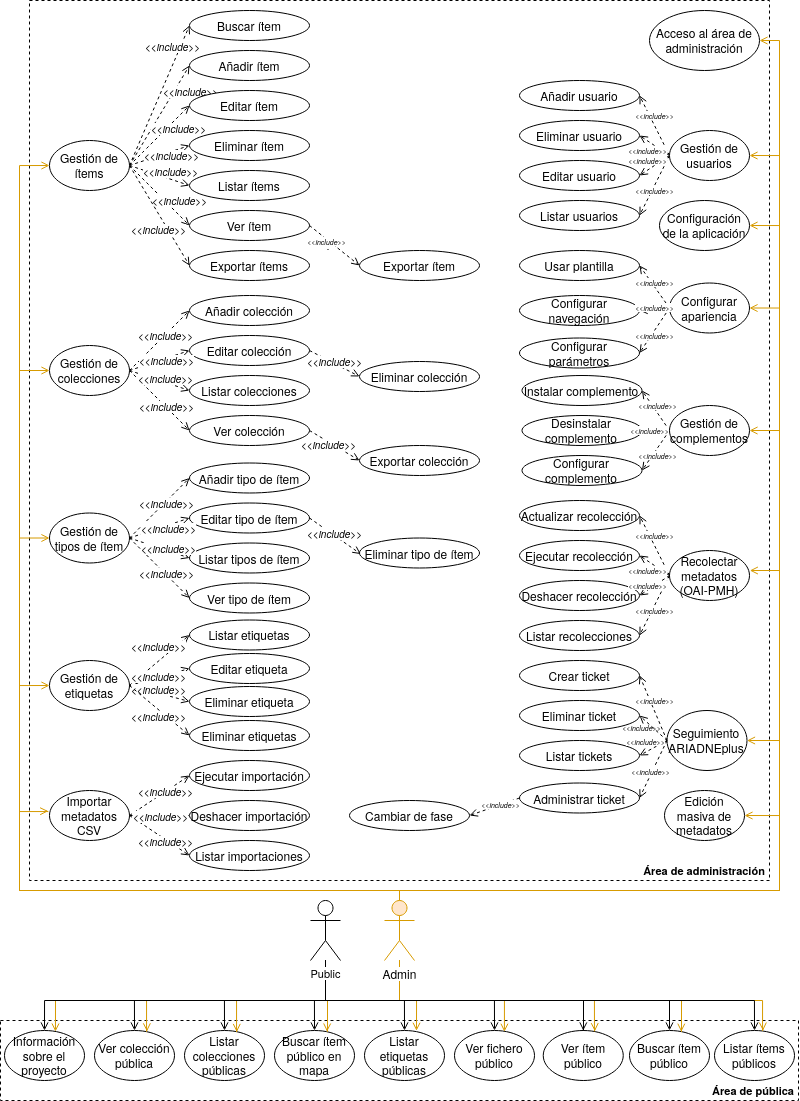
\includegraphics{../_static/images/use-cases-uml.png}
\caption{Diagrama de casos de la aplicación
completa.}\label{use-cases-uml}
}
\end{figure}

\hypertarget{actores}{%
\subsection{Actores}\label{actores}}

Se han considerado dos actores principales:

\begin{itemize}
\tightlist
\item
  \textbf{Public}: usuarios sin acceso al área de administración.
\item
  \textbf{Admin}: usuarios con acceso al área de administración.
\end{itemize}

\hypertarget{casos-de-uso}{%
\subsection{Casos de uso}\label{casos-de-uso}}

\begin{longtable}[]{@{}ll@{}}
\toprule
\begin{minipage}[b]{0.21\columnwidth}\raggedright
\textbf{CU-01}\strut
\end{minipage} & \begin{minipage}[b]{0.73\columnwidth}\raggedright
\textbf{Buscar ítems públicos}\strut
\end{minipage}\tabularnewline
\midrule
\endhead
\begin{minipage}[t]{0.21\columnwidth}\raggedright
\textbf{Versión}\strut
\end{minipage} & \begin{minipage}[t]{0.73\columnwidth}\raggedright
1.0\strut
\end{minipage}\tabularnewline
\begin{minipage}[t]{0.21\columnwidth}\raggedright
\textbf{Autor}\strut
\end{minipage} & \begin{minipage}[t]{0.73\columnwidth}\raggedright
Gonzalo Cuesta Marín\strut
\end{minipage}\tabularnewline
\begin{minipage}[t]{0.21\columnwidth}\raggedright
\textbf{Requisitos asociados}\strut
\end{minipage} & \begin{minipage}[t]{0.73\columnwidth}\raggedright
RFAP-1\strut
\end{minipage}\tabularnewline
\begin{minipage}[t]{0.21\columnwidth}\raggedright
\textbf{Descripción}\strut
\end{minipage} & \begin{minipage}[t]{0.73\columnwidth}\raggedright
Permite al usuario buscar objetos digitales públicos en la
plataforma.\strut
\end{minipage}\tabularnewline
\begin{minipage}[t]{0.21\columnwidth}\raggedright
\textbf{Precondición}\strut
\end{minipage} & \begin{minipage}[t]{0.73\columnwidth}\raggedright
Servidor y base de datos disponible.\strut
\end{minipage}\tabularnewline
\begin{minipage}[t]{0.21\columnwidth}\raggedright
\textbf{Acciones}\strut
\end{minipage} & \begin{minipage}[t]{0.73\columnwidth}\raggedright
\begin{enumerate}
\def\labelenumi{\arabic{enumi}.}
\tightlist
\item
  El usuario introduce texto sobre el campo "Search".
\item
  El usuario presiona la tecla "Enter".
\item
  Se muestran todos los resultados (ítems).
\end{enumerate}\strut
\end{minipage}\tabularnewline
\begin{minipage}[t]{0.21\columnwidth}\raggedright
\textbf{Postcondición}\strut
\end{minipage} & \begin{minipage}[t]{0.73\columnwidth}\raggedright
Todos los ítems resultantes presentan coincidencias con el campo de
texto introducido.\strut
\end{minipage}\tabularnewline
\begin{minipage}[t]{0.21\columnwidth}\raggedright
\textbf{Excepciones}\strut
\end{minipage} & \begin{minipage}[t]{0.73\columnwidth}\raggedright
\begin{itemize}
\tightlist
\item
  Ningún ítem encontrado (mensaje).
\end{itemize}\strut
\end{minipage}\tabularnewline
\begin{minipage}[t]{0.21\columnwidth}\raggedright
\textbf{Importancia}\strut
\end{minipage} & \begin{minipage}[t]{0.73\columnwidth}\raggedright
Alta\strut
\end{minipage}\tabularnewline
\bottomrule
\end{longtable}

\begin{longtable}[]{@{}ll@{}}
\toprule
\begin{minipage}[b]{0.20\columnwidth}\raggedright
\textbf{CU-02}\strut
\end{minipage} & \begin{minipage}[b]{0.74\columnwidth}\raggedright
\textbf{Listar ítems públicos}\strut
\end{minipage}\tabularnewline
\midrule
\endhead
\begin{minipage}[t]{0.20\columnwidth}\raggedright
\textbf{Versión}\strut
\end{minipage} & \begin{minipage}[t]{0.74\columnwidth}\raggedright
1.0\strut
\end{minipage}\tabularnewline
\begin{minipage}[t]{0.20\columnwidth}\raggedright
\textbf{Autor}\strut
\end{minipage} & \begin{minipage}[t]{0.74\columnwidth}\raggedright
Gonzalo Cuesta Marín\strut
\end{minipage}\tabularnewline
\begin{minipage}[t]{0.20\columnwidth}\raggedright
\textbf{Requisitos asociados}\strut
\end{minipage} & \begin{minipage}[t]{0.74\columnwidth}\raggedright
RFAP-3\strut
\end{minipage}\tabularnewline
\begin{minipage}[t]{0.20\columnwidth}\raggedright
\textbf{Descripción}\strut
\end{minipage} & \begin{minipage}[t]{0.74\columnwidth}\raggedright
Permite al usuario ver una lista de todos los ítems públicos en la
plataforma.\strut
\end{minipage}\tabularnewline
\begin{minipage}[t]{0.20\columnwidth}\raggedright
\textbf{Precondición}\strut
\end{minipage} & \begin{minipage}[t]{0.74\columnwidth}\raggedright
Servidor y base de datos disponible.\strut
\end{minipage}\tabularnewline
\begin{minipage}[t]{0.20\columnwidth}\raggedright
\textbf{Acciones}\strut
\end{minipage} & \begin{minipage}[t]{0.74\columnwidth}\raggedright
\begin{enumerate}
\def\labelenumi{\arabic{enumi}.}
\tightlist
\item
  El usuario pulsa sobre el botón "Menu".
\item
  Se muestran todas las entradas del menú de navegación público.
\item
  El usuario pulsa sobre la entrada "Browse Items".
\item
  Se muestra una lista con todos los ítems públicos de la plataforma.
\end{enumerate}\strut
\end{minipage}\tabularnewline
\begin{minipage}[t]{0.20\columnwidth}\raggedright
\textbf{Postcondición}\strut
\end{minipage} & \begin{minipage}[t]{0.74\columnwidth}\raggedright
El número de ítems mostrado es igual al número de ítems públicos
almacenado en la base de datos.\strut
\end{minipage}\tabularnewline
\begin{minipage}[t]{0.20\columnwidth}\raggedright
\textbf{Excepciones}\strut
\end{minipage} & \begin{minipage}[t]{0.74\columnwidth}\raggedright
\begin{itemize}
\tightlist
\item
  No existe ningún ítem público (vista especial).
\end{itemize}\strut
\end{minipage}\tabularnewline
\begin{minipage}[t]{0.20\columnwidth}\raggedright
\textbf{Importancia}\strut
\end{minipage} & \begin{minipage}[t]{0.74\columnwidth}\raggedright
Alta\strut
\end{minipage}\tabularnewline
\bottomrule
\end{longtable}

\begin{longtable}[]{@{}ll@{}}
\toprule
\begin{minipage}[b]{0.22\columnwidth}\raggedright
\textbf{CU-03}\strut
\end{minipage} & \begin{minipage}[b]{0.72\columnwidth}\raggedright
\textbf{Listar colecciones públicas}\strut
\end{minipage}\tabularnewline
\midrule
\endhead
\begin{minipage}[t]{0.22\columnwidth}\raggedright
\textbf{Versión}\strut
\end{minipage} & \begin{minipage}[t]{0.72\columnwidth}\raggedright
1.0\strut
\end{minipage}\tabularnewline
\begin{minipage}[t]{0.22\columnwidth}\raggedright
\textbf{Autor}\strut
\end{minipage} & \begin{minipage}[t]{0.72\columnwidth}\raggedright
Gonzalo Cuesta Marín\strut
\end{minipage}\tabularnewline
\begin{minipage}[t]{0.22\columnwidth}\raggedright
\textbf{Requisitos asociados}\strut
\end{minipage} & \begin{minipage}[t]{0.72\columnwidth}\raggedright
RFAP-4\strut
\end{minipage}\tabularnewline
\begin{minipage}[t]{0.22\columnwidth}\raggedright
\textbf{Descripción}\strut
\end{minipage} & \begin{minipage}[t]{0.72\columnwidth}\raggedright
Permite al usuario ver una lista de todas las colecciones públicas en la
plataforma.\strut
\end{minipage}\tabularnewline
\begin{minipage}[t]{0.22\columnwidth}\raggedright
\textbf{Precondición}\strut
\end{minipage} & \begin{minipage}[t]{0.72\columnwidth}\raggedright
Base de datos disponible.\strut
\end{minipage}\tabularnewline
\begin{minipage}[t]{0.22\columnwidth}\raggedright
\textbf{Acciones}\strut
\end{minipage} & \begin{minipage}[t]{0.72\columnwidth}\raggedright
\begin{enumerate}
\def\labelenumi{\arabic{enumi}.}
\tightlist
\item
  El usuario pulsa sobre el botón "Menu".
\item
  Se muestran todas las entradas del menú de navegación público.
\item
  El usuario pulsa sobre la entrada "Browse Collections".
\item
  Se muestra una lista con todas las colecciones públicas de la
  plataforma.
\end{enumerate}\strut
\end{minipage}\tabularnewline
\begin{minipage}[t]{0.22\columnwidth}\raggedright
\textbf{Postcondición}\strut
\end{minipage} & \begin{minipage}[t]{0.72\columnwidth}\raggedright
\strut
\end{minipage}\tabularnewline
\begin{minipage}[t]{0.22\columnwidth}\raggedright
\textbf{Excepciones}\strut
\end{minipage} & \begin{minipage}[t]{0.72\columnwidth}\raggedright
\begin{itemize}
\tightlist
\item
  No existe ninguna colección pública (vista especial).
\end{itemize}\strut
\end{minipage}\tabularnewline
\begin{minipage}[t]{0.22\columnwidth}\raggedright
\textbf{Importancia}\strut
\end{minipage} & \begin{minipage}[t]{0.72\columnwidth}\raggedright
Alta\strut
\end{minipage}\tabularnewline
\bottomrule
\end{longtable}

\begin{longtable}[]{@{}ll@{}}
\toprule
\begin{minipage}[b]{0.22\columnwidth}\raggedright
\textbf{CU-04}\strut
\end{minipage} & \begin{minipage}[b]{0.72\columnwidth}\raggedright
\textbf{Listar etiquetas públicas}\strut
\end{minipage}\tabularnewline
\midrule
\endhead
\begin{minipage}[t]{0.22\columnwidth}\raggedright
\textbf{Versión}\strut
\end{minipage} & \begin{minipage}[t]{0.72\columnwidth}\raggedright
1.0\strut
\end{minipage}\tabularnewline
\begin{minipage}[t]{0.22\columnwidth}\raggedright
\textbf{Autor}\strut
\end{minipage} & \begin{minipage}[t]{0.72\columnwidth}\raggedright
Gonzalo Cuesta Marín\strut
\end{minipage}\tabularnewline
\begin{minipage}[t]{0.22\columnwidth}\raggedright
\textbf{Requisitos asociados}\strut
\end{minipage} & \begin{minipage}[t]{0.72\columnwidth}\raggedright
RFAP-6\strut
\end{minipage}\tabularnewline
\begin{minipage}[t]{0.22\columnwidth}\raggedright
\textbf{Descripción}\strut
\end{minipage} & \begin{minipage}[t]{0.72\columnwidth}\raggedright
Permite al usuario ver una lista de todas las etiquetas almacenadas en
la plataforma.\strut
\end{minipage}\tabularnewline
\begin{minipage}[t]{0.22\columnwidth}\raggedright
\textbf{Precondición}\strut
\end{minipage} & \begin{minipage}[t]{0.72\columnwidth}\raggedright
Base de datos disponible.\strut
\end{minipage}\tabularnewline
\begin{minipage}[t]{0.22\columnwidth}\raggedright
\textbf{Acciones}\strut
\end{minipage} & \begin{minipage}[t]{0.72\columnwidth}\raggedright
\begin{enumerate}
\def\labelenumi{\arabic{enumi}.}
\tightlist
\item
  El usuario pulsa sobre el botón "Browse all tags".
\item
  Se muestra una lista con todas las etiquetas almacenadas en la
  plataforma.
\end{enumerate}\strut
\end{minipage}\tabularnewline
\begin{minipage}[t]{0.22\columnwidth}\raggedright
\textbf{Postcondición}\strut
\end{minipage} & \begin{minipage}[t]{0.72\columnwidth}\raggedright
\strut
\end{minipage}\tabularnewline
\begin{minipage}[t]{0.22\columnwidth}\raggedright
\textbf{Excepciones}\strut
\end{minipage} & \begin{minipage}[t]{0.72\columnwidth}\raggedright
\begin{itemize}
\tightlist
\item
  No existe ninguna etiqueta (vista especial).
\end{itemize}\strut
\end{minipage}\tabularnewline
\begin{minipage}[t]{0.22\columnwidth}\raggedright
\textbf{Importancia}\strut
\end{minipage} & \begin{minipage}[t]{0.72\columnwidth}\raggedright
Alta\strut
\end{minipage}\tabularnewline
\bottomrule
\end{longtable}

\begin{longtable}[]{@{}ll@{}}
\toprule
\begin{minipage}[b]{0.20\columnwidth}\raggedright
\textbf{CU-05}\strut
\end{minipage} & \begin{minipage}[b]{0.74\columnwidth}\raggedright
\textbf{Ver ítem público}\strut
\end{minipage}\tabularnewline
\midrule
\endhead
\begin{minipage}[t]{0.20\columnwidth}\raggedright
\textbf{Versión}\strut
\end{minipage} & \begin{minipage}[t]{0.74\columnwidth}\raggedright
1.0\strut
\end{minipage}\tabularnewline
\begin{minipage}[t]{0.20\columnwidth}\raggedright
\textbf{Autor}\strut
\end{minipage} & \begin{minipage}[t]{0.74\columnwidth}\raggedright
Gonzalo Cuesta Marín\strut
\end{minipage}\tabularnewline
\begin{minipage}[t]{0.20\columnwidth}\raggedright
\textbf{Requisitos asociados}\strut
\end{minipage} & \begin{minipage}[t]{0.74\columnwidth}\raggedright
RFAP-2, RFAP-2.1\strut
\end{minipage}\tabularnewline
\begin{minipage}[t]{0.20\columnwidth}\raggedright
\textbf{Descripción}\strut
\end{minipage} & \begin{minipage}[t]{0.74\columnwidth}\raggedright
Permite al usuario visualizar un ítem público existente.\strut
\end{minipage}\tabularnewline
\begin{minipage}[t]{0.20\columnwidth}\raggedright
\textbf{Precondición}\strut
\end{minipage} & \begin{minipage}[t]{0.74\columnwidth}\raggedright
Servidor y base de datos disponible.

El ítem público a visualizar existe.\strut
\end{minipage}\tabularnewline
\begin{minipage}[t]{0.20\columnwidth}\raggedright
\textbf{Acciones}\strut
\end{minipage} & \begin{minipage}[t]{0.74\columnwidth}\raggedright
\begin{enumerate}
\def\labelenumi{\arabic{enumi}.}
\tightlist
\item
  El usuario pulsa sobre el título del ítem.
\item
  Se muestra información general del ítem (metadatos, tags, localización
  y cita bibliográfica).
\end{enumerate}\strut
\end{minipage}\tabularnewline
\begin{minipage}[t]{0.20\columnwidth}\raggedright
\textbf{Postcondición}\strut
\end{minipage} & \begin{minipage}[t]{0.74\columnwidth}\raggedright
\strut
\end{minipage}\tabularnewline
\begin{minipage}[t]{0.20\columnwidth}\raggedright
\textbf{Excepciones}\strut
\end{minipage} & \begin{minipage}[t]{0.74\columnwidth}\raggedright
\begin{itemize}
\tightlist
\item
  El ítem no existe (mensaje).
\end{itemize}\strut
\end{minipage}\tabularnewline
\begin{minipage}[t]{0.20\columnwidth}\raggedright
\textbf{Importancia}\strut
\end{minipage} & \begin{minipage}[t]{0.74\columnwidth}\raggedright
Alta\strut
\end{minipage}\tabularnewline
\bottomrule
\end{longtable}

\begin{longtable}[]{@{}ll@{}}
\toprule
\begin{minipage}[b]{0.25\columnwidth}\raggedright
\textbf{CU-06}\strut
\end{minipage} & \begin{minipage}[b]{0.69\columnwidth}\raggedright
\textbf{Ver colección pública}\strut
\end{minipage}\tabularnewline
\midrule
\endhead
\begin{minipage}[t]{0.25\columnwidth}\raggedright
\textbf{Versión}\strut
\end{minipage} & \begin{minipage}[t]{0.69\columnwidth}\raggedright
1.0\strut
\end{minipage}\tabularnewline
\begin{minipage}[t]{0.25\columnwidth}\raggedright
\textbf{Autor}\strut
\end{minipage} & \begin{minipage}[t]{0.69\columnwidth}\raggedright
Gonzalo Cuesta Marín\strut
\end{minipage}\tabularnewline
\begin{minipage}[t]{0.25\columnwidth}\raggedright
\textbf{Requisitos asociados}\strut
\end{minipage} & \begin{minipage}[t]{0.69\columnwidth}\raggedright
RFAP-5\strut
\end{minipage}\tabularnewline
\begin{minipage}[t]{0.25\columnwidth}\raggedright
\textbf{Descripción}\strut
\end{minipage} & \begin{minipage}[t]{0.69\columnwidth}\raggedright
Permite al usuario visualizar un ítem público existente.\strut
\end{minipage}\tabularnewline
\begin{minipage}[t]{0.25\columnwidth}\raggedright
\textbf{Precondición}\strut
\end{minipage} & \begin{minipage}[t]{0.69\columnwidth}\raggedright
Servidor y base de datos disponible.

La colección pública a visualizar existe.\strut
\end{minipage}\tabularnewline
\begin{minipage}[t]{0.25\columnwidth}\raggedright
\textbf{Acciones}\strut
\end{minipage} & \begin{minipage}[t]{0.69\columnwidth}\raggedright
\begin{enumerate}
\def\labelenumi{\arabic{enumi}.}
\tightlist
\item
  El usuario pulsa sobre el título de la colección.
\item
  Se muestra el título de la colección.
\item
  Se muestra un botón para acceder a la lista de ítems de la colección.
\end{enumerate}\strut
\end{minipage}\tabularnewline
\begin{minipage}[t]{0.25\columnwidth}\raggedright
\textbf{Postcondición}\strut
\end{minipage} & \begin{minipage}[t]{0.69\columnwidth}\raggedright
\strut
\end{minipage}\tabularnewline
\begin{minipage}[t]{0.25\columnwidth}\raggedright
\textbf{Excepciones}\strut
\end{minipage} & \begin{minipage}[t]{0.69\columnwidth}\raggedright
\begin{itemize}
\tightlist
\item
  La colección no existe (mensaje).
\end{itemize}\strut
\end{minipage}\tabularnewline
\begin{minipage}[t]{0.25\columnwidth}\raggedright
\textbf{Importancia}\strut
\end{minipage} & \begin{minipage}[t]{0.69\columnwidth}\raggedright
Alta\strut
\end{minipage}\tabularnewline
\bottomrule
\end{longtable}

\begin{longtable}[]{@{}ll@{}}
\toprule
\begin{minipage}[b]{0.23\columnwidth}\raggedright
\textbf{CU-07}\strut
\end{minipage} & \begin{minipage}[b]{0.71\columnwidth}\raggedright
\textbf{Ver fichero público}\strut
\end{minipage}\tabularnewline
\midrule
\endhead
\begin{minipage}[t]{0.23\columnwidth}\raggedright
\textbf{Versión}\strut
\end{minipage} & \begin{minipage}[t]{0.71\columnwidth}\raggedright
1.0\strut
\end{minipage}\tabularnewline
\begin{minipage}[t]{0.23\columnwidth}\raggedright
\textbf{Autor}\strut
\end{minipage} & \begin{minipage}[t]{0.71\columnwidth}\raggedright
Gonzalo Cuesta Marín\strut
\end{minipage}\tabularnewline
\begin{minipage}[t]{0.23\columnwidth}\raggedright
\textbf{Requisitos asociados}\strut
\end{minipage} & \begin{minipage}[t]{0.71\columnwidth}\raggedright
RFAP-2.1\strut
\end{minipage}\tabularnewline
\begin{minipage}[t]{0.23\columnwidth}\raggedright
\textbf{Descripción}\strut
\end{minipage} & \begin{minipage}[t]{0.71\columnwidth}\raggedright
Permite al usuario visualizar el fichero de un ítem público
existente.\strut
\end{minipage}\tabularnewline
\begin{minipage}[t]{0.23\columnwidth}\raggedright
\textbf{Precondición}\strut
\end{minipage} & \begin{minipage}[t]{0.71\columnwidth}\raggedright
Servidor y base de datos disponible.

El ítem público asociado al fichero existe.\strut
\end{minipage}\tabularnewline
\begin{minipage}[t]{0.23\columnwidth}\raggedright
\textbf{Acciones}\strut
\end{minipage} & \begin{minipage}[t]{0.71\columnwidth}\raggedright
\begin{enumerate}
\def\labelenumi{\arabic{enumi}.}
\tightlist
\item
  El usuario pulsa sobre el nombre del fichero.
\item
  Se muestra información general del fichero (nombre, metadatos e ítem
  asociado).
\end{enumerate}\strut
\end{minipage}\tabularnewline
\begin{minipage}[t]{0.23\columnwidth}\raggedright
\textbf{Postcondición}\strut
\end{minipage} & \begin{minipage}[t]{0.71\columnwidth}\raggedright
\strut
\end{minipage}\tabularnewline
\begin{minipage}[t]{0.23\columnwidth}\raggedright
\textbf{Excepciones}\strut
\end{minipage} & \begin{minipage}[t]{0.71\columnwidth}\raggedright
\begin{itemize}
\tightlist
\item
  El fichero no existe (mensaje).
\end{itemize}\strut
\end{minipage}\tabularnewline
\begin{minipage}[t]{0.23\columnwidth}\raggedright
\textbf{Importancia}\strut
\end{minipage} & \begin{minipage}[t]{0.71\columnwidth}\raggedright
Alta\strut
\end{minipage}\tabularnewline
\bottomrule
\end{longtable}

\begin{longtable}[]{@{}ll@{}}
\toprule
\begin{minipage}[b]{0.20\columnwidth}\raggedright
\textbf{CU-08}\strut
\end{minipage} & \begin{minipage}[b]{0.74\columnwidth}\raggedright
\textbf{Buscar ítem público en mapa}\strut
\end{minipage}\tabularnewline
\midrule
\endhead
\begin{minipage}[t]{0.20\columnwidth}\raggedright
\textbf{Versión}\strut
\end{minipage} & \begin{minipage}[t]{0.74\columnwidth}\raggedright
1.0\strut
\end{minipage}\tabularnewline
\begin{minipage}[t]{0.20\columnwidth}\raggedright
\textbf{Autor}\strut
\end{minipage} & \begin{minipage}[t]{0.74\columnwidth}\raggedright
Gonzalo Cuesta Marín\strut
\end{minipage}\tabularnewline
\begin{minipage}[t]{0.20\columnwidth}\raggedright
\textbf{Requisitos asociados}\strut
\end{minipage} & \begin{minipage}[t]{0.74\columnwidth}\raggedright
RFAP-7\strut
\end{minipage}\tabularnewline
\begin{minipage}[t]{0.20\columnwidth}\raggedright
\textbf{Descripción}\strut
\end{minipage} & \begin{minipage}[t]{0.74\columnwidth}\raggedright
Permite al usuario buscar objetos digitales públicos en la
plataforma.\strut
\end{minipage}\tabularnewline
\begin{minipage}[t]{0.20\columnwidth}\raggedright
\textbf{Precondición}\strut
\end{minipage} & \begin{minipage}[t]{0.74\columnwidth}\raggedright
Servidor y base de datos disponible.\strut
\end{minipage}\tabularnewline
\begin{minipage}[t]{0.20\columnwidth}\raggedright
\textbf{Acciones}\strut
\end{minipage} & \begin{minipage}[t]{0.74\columnwidth}\raggedright
\begin{enumerate}
\def\labelenumi{\arabic{enumi}.}
\tightlist
\item
  El usuario se desplaza a la localización deseada arrastrando el cursor
  por el mapa.
\item
  El usuario ajusta el zoom para una búsqueda más precisa (opcional).
\item
  El usuario cambia la plantilla del mapa (opcional).
\item
  Se muestran los ítems, en forma de marcador, que estén ubicados en la
  zona geográfica fijada.
\item
  El usuario pulsa sobre un marcador (ítem).
\item
  Se muestra un bocadillo con información mínima del ítem (título).
\end{enumerate}\strut
\end{minipage}\tabularnewline
\begin{minipage}[t]{0.20\columnwidth}\raggedright
\textbf{Postcondición}\strut
\end{minipage} & \begin{minipage}[t]{0.74\columnwidth}\raggedright
\strut
\end{minipage}\tabularnewline
\begin{minipage}[t]{0.20\columnwidth}\raggedright
\textbf{Excepciones}\strut
\end{minipage} & \begin{minipage}[t]{0.74\columnwidth}\raggedright
\strut
\end{minipage}\tabularnewline
\begin{minipage}[t]{0.20\columnwidth}\raggedright
\textbf{Importancia}\strut
\end{minipage} & \begin{minipage}[t]{0.74\columnwidth}\raggedright
Alta\strut
\end{minipage}\tabularnewline
\bottomrule
\end{longtable}

\begin{longtable}[]{@{}ll@{}}
\toprule
\begin{minipage}[b]{0.27\columnwidth}\raggedright
\textbf{CU-09}\strut
\end{minipage} & \begin{minipage}[b]{0.67\columnwidth}\raggedright
\textbf{Información del proyecto}\strut
\end{minipage}\tabularnewline
\midrule
\endhead
\begin{minipage}[t]{0.27\columnwidth}\raggedright
\textbf{Versión}\strut
\end{minipage} & \begin{minipage}[t]{0.67\columnwidth}\raggedright
1.0\strut
\end{minipage}\tabularnewline
\begin{minipage}[t]{0.27\columnwidth}\raggedright
\textbf{Autor}\strut
\end{minipage} & \begin{minipage}[t]{0.67\columnwidth}\raggedright
Gonzalo Cuesta Marín\strut
\end{minipage}\tabularnewline
\begin{minipage}[t]{0.27\columnwidth}\raggedright
\textbf{Requisitos asociados}\strut
\end{minipage} & \begin{minipage}[t]{0.67\columnwidth}\raggedright
RFAP-8\strut
\end{minipage}\tabularnewline
\begin{minipage}[t]{0.27\columnwidth}\raggedright
\textbf{Descripción}\strut
\end{minipage} & \begin{minipage}[t]{0.67\columnwidth}\raggedright
Permite al usuario conocer más información acerca del proyecto.\strut
\end{minipage}\tabularnewline
\begin{minipage}[t]{0.27\columnwidth}\raggedright
\textbf{Precondición}\strut
\end{minipage} & \begin{minipage}[t]{0.67\columnwidth}\raggedright
Base de datos disponible.\strut
\end{minipage}\tabularnewline
\begin{minipage}[t]{0.27\columnwidth}\raggedright
\textbf{Acciones}\strut
\end{minipage} & \begin{minipage}[t]{0.67\columnwidth}\raggedright
\begin{enumerate}
\def\labelenumi{\arabic{enumi}.}
\tightlist
\item
  El usuario pulsa sobre el botón "Menu".
\item
  Se muestran todas las entradas del menú de navegación público.
\item
  El usuario pulsa sobre la entrada "About".
\item
  Se muestran la información general del proyecto
\end{enumerate}\strut
\end{minipage}\tabularnewline
\begin{minipage}[t]{0.27\columnwidth}\raggedright
\textbf{Postcondición}\strut
\end{minipage} & \begin{minipage}[t]{0.67\columnwidth}\raggedright
\strut
\end{minipage}\tabularnewline
\begin{minipage}[t]{0.27\columnwidth}\raggedright
\textbf{Excepciones}\strut
\end{minipage} & \begin{minipage}[t]{0.67\columnwidth}\raggedright
\strut
\end{minipage}\tabularnewline
\begin{minipage}[t]{0.27\columnwidth}\raggedright
\textbf{Importancia}\strut
\end{minipage} & \begin{minipage}[t]{0.67\columnwidth}\raggedright
Media\strut
\end{minipage}\tabularnewline
\bottomrule
\end{longtable}

\begin{longtable}[]{@{}ll@{}}
\toprule
\begin{minipage}[b]{0.20\columnwidth}\raggedright
\textbf{CU-10}\strut
\end{minipage} & \begin{minipage}[b]{0.74\columnwidth}\raggedright
\textbf{Acceso al área de administración}\strut
\end{minipage}\tabularnewline
\midrule
\endhead
\begin{minipage}[t]{0.20\columnwidth}\raggedright
\textbf{Versión}\strut
\end{minipage} & \begin{minipage}[t]{0.74\columnwidth}\raggedright
1.0\strut
\end{minipage}\tabularnewline
\begin{minipage}[t]{0.20\columnwidth}\raggedright
\textbf{Autor}\strut
\end{minipage} & \begin{minipage}[t]{0.74\columnwidth}\raggedright
Gonzalo Cuesta Marín\strut
\end{minipage}\tabularnewline
\begin{minipage}[t]{0.20\columnwidth}\raggedright
\textbf{Requisitos asociados}\strut
\end{minipage} & \begin{minipage}[t]{0.74\columnwidth}\raggedright
RFAA-1\strut
\end{minipage}\tabularnewline
\begin{minipage}[t]{0.20\columnwidth}\raggedright
\textbf{Descripción}\strut
\end{minipage} & \begin{minipage}[t]{0.74\columnwidth}\raggedright
Permite al usuario acceder al área de administración.\strut
\end{minipage}\tabularnewline
\begin{minipage}[t]{0.20\columnwidth}\raggedright
\textbf{Precondición}\strut
\end{minipage} & \begin{minipage}[t]{0.74\columnwidth}\raggedright
Servidor y base de datos disponible.\strut
\end{minipage}\tabularnewline
\begin{minipage}[t]{0.20\columnwidth}\raggedright
\textbf{Acciones}\strut
\end{minipage} & \begin{minipage}[t]{0.74\columnwidth}\raggedright
\begin{enumerate}
\def\labelenumi{\arabic{enumi}.}
\tightlist
\item
  Se muestra al usuario el formulario de inicio de sesión.
\item
  El usuario introduce su nombre de usuario.
\item
  El usuario introduce su contraseña de usuario.
\item
  El usuario pulsa sobre el botón "Login".
\item
  Si los datos son correctos, se traslada al usuario al interior del
  área de administración.
\end{enumerate}\strut
\end{minipage}\tabularnewline
\begin{minipage}[t]{0.20\columnwidth}\raggedright
\textbf{Postcondición}\strut
\end{minipage} & \begin{minipage}[t]{0.74\columnwidth}\raggedright
El usuario accede a la pantalla principal del área de
administración\strut
\end{minipage}\tabularnewline
\begin{minipage}[t]{0.20\columnwidth}\raggedright
\textbf{Excepciones}\strut
\end{minipage} & \begin{minipage}[t]{0.74\columnwidth}\raggedright
\begin{itemize}
\tightlist
\item
  Nombre de usuario o contraseña incorrectos (mensaje).
\item
  Usuario inactivo (mensaje).
\end{itemize}\strut
\end{minipage}\tabularnewline
\begin{minipage}[t]{0.20\columnwidth}\raggedright
\textbf{Importancia}\strut
\end{minipage} & \begin{minipage}[t]{0.74\columnwidth}\raggedright
Alta\strut
\end{minipage}\tabularnewline
\bottomrule
\end{longtable}

\begin{longtable}[]{@{}ll@{}}
\toprule
\begin{minipage}[b]{0.21\columnwidth}\raggedright
\textbf{CU-11}\strut
\end{minipage} & \begin{minipage}[b]{0.73\columnwidth}\raggedright
\textbf{Gestión de ítems}\strut
\end{minipage}\tabularnewline
\midrule
\endhead
\begin{minipage}[t]{0.21\columnwidth}\raggedright
\textbf{Versión}\strut
\end{minipage} & \begin{minipage}[t]{0.73\columnwidth}\raggedright
1.0\strut
\end{minipage}\tabularnewline
\begin{minipage}[t]{0.21\columnwidth}\raggedright
\textbf{Autor}\strut
\end{minipage} & \begin{minipage}[t]{0.73\columnwidth}\raggedright
Gonzalo Cuesta Marín\strut
\end{minipage}\tabularnewline
\begin{minipage}[t]{0.21\columnwidth}\raggedright
\textbf{Requisitos asociados}\strut
\end{minipage} & \begin{minipage}[t]{0.73\columnwidth}\raggedright
RFAA-2, RFAA-2.1, RFAA-2.2, RFAA-2.3, RFAA-2.4, RFAA-2.5, RFAA-2.5.1,
RFAA-2.6, RFAA-2.7\strut
\end{minipage}\tabularnewline
\begin{minipage}[t]{0.21\columnwidth}\raggedright
\textbf{Descripción}\strut
\end{minipage} & \begin{minipage}[t]{0.73\columnwidth}\raggedright
Permite al usuario gestionar ítems.\strut
\end{minipage}\tabularnewline
\begin{minipage}[t]{0.21\columnwidth}\raggedright
\textbf{Precondición}\strut
\end{minipage} & \begin{minipage}[t]{0.73\columnwidth}\raggedright
Servidor y base de datos disponible.

Sesión iniciada en área de administración.\strut
\end{minipage}\tabularnewline
\begin{minipage}[t]{0.21\columnwidth}\raggedright
\textbf{Acciones}\strut
\end{minipage} & \begin{minipage}[t]{0.73\columnwidth}\raggedright
\begin{enumerate}
\def\labelenumi{\arabic{enumi}.}
\tightlist
\item
  El usuario pulsa sobre la entrada "Items" del submenú "Data Manager"
  del menú principal.
\item
  Se listan los ítems.
\item
  Por cada ítem se da la opción de ver en detalle, editar o eliminar.
\item
  Se muestra un botón para añadir un ítem.
\item
  Se muestra un botón y un desplegable para buscar o filtrar ítems.
\item
  Se muestran múltiples formatos de exportación disponibles.
\end{enumerate}\strut
\end{minipage}\tabularnewline
\begin{minipage}[t]{0.21\columnwidth}\raggedright
\textbf{Postcondición}\strut
\end{minipage} & \begin{minipage}[t]{0.73\columnwidth}\raggedright
El número de ítems listado es igual al número de ítems almacenado en la
base de datos\strut
\end{minipage}\tabularnewline
\begin{minipage}[t]{0.21\columnwidth}\raggedright
\textbf{Excepciones}\strut
\end{minipage} & \begin{minipage}[t]{0.73\columnwidth}\raggedright
\begin{itemize}
\tightlist
\item
  Error al cargar ítems (mensaje).
\item
  No existe ningún mensaje (vista especial)
\end{itemize}\strut
\end{minipage}\tabularnewline
\begin{minipage}[t]{0.21\columnwidth}\raggedright
\textbf{Importancia}\strut
\end{minipage} & \begin{minipage}[t]{0.73\columnwidth}\raggedright
Alta\strut
\end{minipage}\tabularnewline
\bottomrule
\end{longtable}

\begin{longtable}[]{@{}ll@{}}
\toprule
\begin{minipage}[b]{0.15\columnwidth}\raggedright
\textbf{CU-12}\strut
\end{minipage} & \begin{minipage}[b]{0.79\columnwidth}\raggedright
\textbf{Añadir ítem}\strut
\end{minipage}\tabularnewline
\midrule
\endhead
\begin{minipage}[t]{0.15\columnwidth}\raggedright
\textbf{Versión}\strut
\end{minipage} & \begin{minipage}[t]{0.79\columnwidth}\raggedright
1.0\strut
\end{minipage}\tabularnewline
\begin{minipage}[t]{0.15\columnwidth}\raggedright
\textbf{Autor}\strut
\end{minipage} & \begin{minipage}[t]{0.79\columnwidth}\raggedright
Gonzalo Cuesta Marín\strut
\end{minipage}\tabularnewline
\begin{minipage}[t]{0.15\columnwidth}\raggedright
\textbf{Requisitos asociados}\strut
\end{minipage} & \begin{minipage}[t]{0.79\columnwidth}\raggedright
RFAA-2.1\strut
\end{minipage}\tabularnewline
\begin{minipage}[t]{0.15\columnwidth}\raggedright
\textbf{Descripción}\strut
\end{minipage} & \begin{minipage}[t]{0.79\columnwidth}\raggedright
Permite al usuario añadir un nuevo ítem.\strut
\end{minipage}\tabularnewline
\begin{minipage}[t]{0.15\columnwidth}\raggedright
\textbf{Precondición}\strut
\end{minipage} & \begin{minipage}[t]{0.79\columnwidth}\raggedright
Servidor y base de datos disponible.\strut
\end{minipage}\tabularnewline
\begin{minipage}[t]{0.15\columnwidth}\raggedright
\textbf{Acciones}\strut
\end{minipage} & \begin{minipage}[t]{0.79\columnwidth}\raggedright
\begin{enumerate}
\def\labelenumi{\arabic{enumi}.}
\tightlist
\item
  El usuario pulsa sobre el botón "Add an Item".
\item
  Se muestra al usuario una ventana con varios formularios divididos en
  pestañas y varios botones.
\item
  El usuario pulsa sobre la pestaña "Dublin Core" para añadir metadatos
  estandarizados (opcional).
\item
  El usuario pulsa sobre la pestaña "Item Type Metadata" para añadir
  metadatos específicos (opcional).
\item
  El usuario pulsa sobre la pestaña "Files" para añadir ficheros
  (opcional).
\item
  El usuario pulsa sobre la pestaña "Tags" para añadir etiquetas
  (opcional).
\item
  El usuario pulsa sobre la pestaña "Map" para añadir una localización
  (opcional).
\item
  El usuario marca la casilla "Public" para hacerlo público (opcional).
\item
  El usuario marca la casilla "Feature" para hacerlo destacado
  (opcional).
\item
  El usuario selecciona la colección a la que pertenece (opcional).
\item
  El usuario pulsa el botón "Add Item".
\item
  Si no hay ningún error, se guarda un nuevo ítem junto a los demás
  objetos asociados.
\end{enumerate}\strut
\end{minipage}\tabularnewline
\begin{minipage}[t]{0.15\columnwidth}\raggedright
\textbf{Postcondición}\strut
\end{minipage} & \begin{minipage}[t]{0.79\columnwidth}\raggedright
Existe un ítem más en la base de datos.\strut
\end{minipage}\tabularnewline
\begin{minipage}[t]{0.15\columnwidth}\raggedright
\textbf{Excepciones}\strut
\end{minipage} & \begin{minipage}[t]{0.79\columnwidth}\raggedright
\begin{itemize}
\tightlist
\item
  Error al crear ítem (mensaje).
\item
  Error con el tipo de fichero introducido (mensaje).
\end{itemize}\strut
\end{minipage}\tabularnewline
\begin{minipage}[t]{0.15\columnwidth}\raggedright
\textbf{Importancia}\strut
\end{minipage} & \begin{minipage}[t]{0.79\columnwidth}\raggedright
Alta\strut
\end{minipage}\tabularnewline
\bottomrule
\end{longtable}

\begin{longtable}[]{@{}ll@{}}
\toprule
\begin{minipage}[b]{0.15\columnwidth}\raggedright
\textbf{CU-13}\strut
\end{minipage} & \begin{minipage}[b]{0.79\columnwidth}\raggedright
\textbf{Editar ítem}\strut
\end{minipage}\tabularnewline
\midrule
\endhead
\begin{minipage}[t]{0.15\columnwidth}\raggedright
\textbf{Versión}\strut
\end{minipage} & \begin{minipage}[t]{0.79\columnwidth}\raggedright
1.0\strut
\end{minipage}\tabularnewline
\begin{minipage}[t]{0.15\columnwidth}\raggedright
\textbf{Autor}\strut
\end{minipage} & \begin{minipage}[t]{0.79\columnwidth}\raggedright
Gonzalo Cuesta Marín\strut
\end{minipage}\tabularnewline
\begin{minipage}[t]{0.15\columnwidth}\raggedright
\textbf{Requisitos asociados}\strut
\end{minipage} & \begin{minipage}[t]{0.79\columnwidth}\raggedright
RFAA-2.2\strut
\end{minipage}\tabularnewline
\begin{minipage}[t]{0.15\columnwidth}\raggedright
\textbf{Descripción}\strut
\end{minipage} & \begin{minipage}[t]{0.79\columnwidth}\raggedright
Permite al usuario editar un ítem existente.\strut
\end{minipage}\tabularnewline
\begin{minipage}[t]{0.15\columnwidth}\raggedright
\textbf{Precondición}\strut
\end{minipage} & \begin{minipage}[t]{0.79\columnwidth}\raggedright
Servidor y base de datos disponible.

El ítem a editar existe.\strut
\end{minipage}\tabularnewline
\begin{minipage}[t]{0.15\columnwidth}\raggedright
\textbf{Acciones}\strut
\end{minipage} & \begin{minipage}[t]{0.79\columnwidth}\raggedright
\begin{enumerate}
\def\labelenumi{\arabic{enumi}.}
\tightlist
\item
  El usuario pulsa sobre el elemento "Edit" del ítem que va a editar.
\item
  Se muestra al usuario una ventana con varios formularios divididos en
  pestañas y tres botones (guardar, ver en área pública y eliminar).
\item
  El usuario pulsa sobre la pestaña "Dublin Core" para editar metadatos
  estandarizados (opcional).
\item
  El usuario pulsa sobre la pestaña "Item Type Metadata" para editar
  metadatos específicos (opcional).
\item
  El usuario pulsa sobre la pestaña "Files" para editar ficheros
  (opcional).
\item
  El usuario pulsa sobre la pestaña "Map" para editar una localización
  (opcional).
\item
  El usuario modifica el estado de la casilla "Public" para hacerlo
  público/privado (opcional).
\item
  El usuario modifica el estado de la casilla "Feature" para hacerlo o
  no destacado (opcional).
\item
  El usuario modifica la colección a la que pertenece (opcional).
\item
  El usuario pulsa el botón "Save Changes".
\item
  Si no hay ningún error, se actualiza el ítem junto a todos sus objetos
  asociados (metadatos/ficheros/etiquetas/localización).
\end{enumerate}\strut
\end{minipage}\tabularnewline
\begin{minipage}[t]{0.15\columnwidth}\raggedright
\textbf{Postcondición}\strut
\end{minipage} & \begin{minipage}[t]{0.79\columnwidth}\raggedright
La información del ítem y de todos sus objetos asociados ha sido
actualizada.\strut
\end{minipage}\tabularnewline
\begin{minipage}[t]{0.15\columnwidth}\raggedright
\textbf{Excepciones}\strut
\end{minipage} & \begin{minipage}[t]{0.79\columnwidth}\raggedright
\begin{itemize}
\tightlist
\item
  Error al guardar ítem (mensaje).
\item
  Error con el tipo de fichero introducido (mensaje).
\end{itemize}\strut
\end{minipage}\tabularnewline
\begin{minipage}[t]{0.15\columnwidth}\raggedright
\textbf{Importancia}\strut
\end{minipage} & \begin{minipage}[t]{0.79\columnwidth}\raggedright
Alta\strut
\end{minipage}\tabularnewline
\bottomrule
\end{longtable}

\begin{longtable}[]{@{}ll@{}}
\toprule
\begin{minipage}[b]{0.20\columnwidth}\raggedright
\textbf{CU-14}\strut
\end{minipage} & \begin{minipage}[b]{0.74\columnwidth}\raggedright
\textbf{Eliminar ítem}\strut
\end{minipage}\tabularnewline
\midrule
\endhead
\begin{minipage}[t]{0.20\columnwidth}\raggedright
\textbf{Versión}\strut
\end{minipage} & \begin{minipage}[t]{0.74\columnwidth}\raggedright
1.0\strut
\end{minipage}\tabularnewline
\begin{minipage}[t]{0.20\columnwidth}\raggedright
\textbf{Autor}\strut
\end{minipage} & \begin{minipage}[t]{0.74\columnwidth}\raggedright
Gonzalo Cuesta Marín\strut
\end{minipage}\tabularnewline
\begin{minipage}[t]{0.20\columnwidth}\raggedright
\textbf{Requisitos asociados}\strut
\end{minipage} & \begin{minipage}[t]{0.74\columnwidth}\raggedright
RFAA-2.3\strut
\end{minipage}\tabularnewline
\begin{minipage}[t]{0.20\columnwidth}\raggedright
\textbf{Descripción}\strut
\end{minipage} & \begin{minipage}[t]{0.74\columnwidth}\raggedright
Permite al usuario eliminar un ítem existente.\strut
\end{minipage}\tabularnewline
\begin{minipage}[t]{0.20\columnwidth}\raggedright
\textbf{Precondición}\strut
\end{minipage} & \begin{minipage}[t]{0.74\columnwidth}\raggedright
Servidor y base de datos disponible.

El ítem a eliminar existe.\strut
\end{minipage}\tabularnewline
\begin{minipage}[t]{0.20\columnwidth}\raggedright
\textbf{Acciones}\strut
\end{minipage} & \begin{minipage}[t]{0.74\columnwidth}\raggedright
\begin{enumerate}
\def\labelenumi{\arabic{enumi}.}
\tightlist
\item
  El usuario pulsa sobre "Delete".
\item
  Se muestra al usuario un mensaje de confirmación.
\item
  El usuario pulsa sobre el botón "Delete" para confirmar la
  eliminación.
\item
  Se elimina el ítem de la vista.
\item
  Se informa al usuario que el ítem ha sido eliminado correctamente.
\end{enumerate}\strut
\end{minipage}\tabularnewline
\begin{minipage}[t]{0.20\columnwidth}\raggedright
\textbf{Postcondición}\strut
\end{minipage} & \begin{minipage}[t]{0.74\columnwidth}\raggedright
El ítem y sus objetos asociados (metadatos, ficheros y localización) no
existen en la base de datos.\strut
\end{minipage}\tabularnewline
\begin{minipage}[t]{0.20\columnwidth}\raggedright
\textbf{Excepciones}\strut
\end{minipage} & \begin{minipage}[t]{0.74\columnwidth}\raggedright
\begin{itemize}
\tightlist
\item
  Error al eliminar ítem (mensaje).
\end{itemize}\strut
\end{minipage}\tabularnewline
\begin{minipage}[t]{0.20\columnwidth}\raggedright
\textbf{Importancia}\strut
\end{minipage} & \begin{minipage}[t]{0.74\columnwidth}\raggedright
Alta\strut
\end{minipage}\tabularnewline
\bottomrule
\end{longtable}

\begin{longtable}[]{@{}ll@{}}
\toprule
\begin{minipage}[b]{0.19\columnwidth}\raggedright
\textbf{CU-15}\strut
\end{minipage} & \begin{minipage}[b]{0.75\columnwidth}\raggedright
\textbf{Listar ítems}\strut
\end{minipage}\tabularnewline
\midrule
\endhead
\begin{minipage}[t]{0.19\columnwidth}\raggedright
\textbf{Versión}\strut
\end{minipage} & \begin{minipage}[t]{0.75\columnwidth}\raggedright
1.0\strut
\end{minipage}\tabularnewline
\begin{minipage}[t]{0.19\columnwidth}\raggedright
\textbf{Autor}\strut
\end{minipage} & \begin{minipage}[t]{0.75\columnwidth}\raggedright
Gonzalo Cuesta Marín\strut
\end{minipage}\tabularnewline
\begin{minipage}[t]{0.19\columnwidth}\raggedright
\textbf{Requisitos asociados}\strut
\end{minipage} & \begin{minipage}[t]{0.75\columnwidth}\raggedright
RFAA-2.4\strut
\end{minipage}\tabularnewline
\begin{minipage}[t]{0.19\columnwidth}\raggedright
\textbf{Descripción}\strut
\end{minipage} & \begin{minipage}[t]{0.75\columnwidth}\raggedright
Permite al usuario ver una lista de todos los ítems almacenados en la
aplicación.\strut
\end{minipage}\tabularnewline
\begin{minipage}[t]{0.19\columnwidth}\raggedright
\textbf{Precondición}\strut
\end{minipage} & \begin{minipage}[t]{0.75\columnwidth}\raggedright
Servidor y base de datos disponible.\strut
\end{minipage}\tabularnewline
\begin{minipage}[t]{0.19\columnwidth}\raggedright
\textbf{Acciones}\strut
\end{minipage} & \begin{minipage}[t]{0.75\columnwidth}\raggedright
\begin{enumerate}
\def\labelenumi{\arabic{enumi}.}
\tightlist
\item
  El usuario pulsa sobre la entrada "Items" del submenú "Data Manager"
  del menú principal.
\item
  Se muestran los ítems en una tabla indicando su título, creador, tipo
  y fecha de creación.
\item
  Opcionalmente se pueden ordenar los ítems pulsando sobre alguna de las
  cabeceras de la tabla.
\end{enumerate}\strut
\end{minipage}\tabularnewline
\begin{minipage}[t]{0.19\columnwidth}\raggedright
\textbf{Postcondición}\strut
\end{minipage} & \begin{minipage}[t]{0.75\columnwidth}\raggedright
\strut
\end{minipage}\tabularnewline
\begin{minipage}[t]{0.19\columnwidth}\raggedright
\textbf{Excepciones}\strut
\end{minipage} & \begin{minipage}[t]{0.75\columnwidth}\raggedright
\begin{itemize}
\tightlist
\item
  No existen ítems (vista especial).
\end{itemize}\strut
\end{minipage}\tabularnewline
\begin{minipage}[t]{0.19\columnwidth}\raggedright
\textbf{Importancia}\strut
\end{minipage} & \begin{minipage}[t]{0.75\columnwidth}\raggedright
Alta\strut
\end{minipage}\tabularnewline
\bottomrule
\end{longtable}

\begin{longtable}[]{@{}ll@{}}
\toprule
\begin{minipage}[b]{0.24\columnwidth}\raggedright
\textbf{CU-16}\strut
\end{minipage} & \begin{minipage}[b]{0.70\columnwidth}\raggedright
\textbf{Ver ítem}\strut
\end{minipage}\tabularnewline
\midrule
\endhead
\begin{minipage}[t]{0.24\columnwidth}\raggedright
\textbf{Versión}\strut
\end{minipage} & \begin{minipage}[t]{0.70\columnwidth}\raggedright
1.0\strut
\end{minipage}\tabularnewline
\begin{minipage}[t]{0.24\columnwidth}\raggedright
\textbf{Autor}\strut
\end{minipage} & \begin{minipage}[t]{0.70\columnwidth}\raggedright
Gonzalo Cuesta Marín\strut
\end{minipage}\tabularnewline
\begin{minipage}[t]{0.24\columnwidth}\raggedright
\textbf{Requisitos asociados}\strut
\end{minipage} & \begin{minipage}[t]{0.70\columnwidth}\raggedright
RFAA-2.5, RFAA-2.5.1\strut
\end{minipage}\tabularnewline
\begin{minipage}[t]{0.24\columnwidth}\raggedright
\textbf{Descripción}\strut
\end{minipage} & \begin{minipage}[t]{0.70\columnwidth}\raggedright
Permite al usuario visualizar un ítem\strut
\end{minipage}\tabularnewline
\begin{minipage}[t]{0.24\columnwidth}\raggedright
\textbf{Precondición}\strut
\end{minipage} & \begin{minipage}[t]{0.70\columnwidth}\raggedright
Servidor y base de datos disponible.

El ítem a visualizar existe.\strut
\end{minipage}\tabularnewline
\begin{minipage}[t]{0.24\columnwidth}\raggedright
\textbf{Acciones}\strut
\end{minipage} & \begin{minipage}[t]{0.70\columnwidth}\raggedright
\begin{enumerate}
\def\labelenumi{\arabic{enumi}.}
\tightlist
\item
  El usuario pulsa sobre el título del ítem a visualizar.
\item
  Se obtiene la información del ítem (incluída la de sus objetos
  asociados).
\item
  Se muestra información general del ítem.
\item
  Se muestra información de cada uno de los objetos asociados al ítem.

  \begin{enumerate}
  \def\labelenumii{\alph{enumii}.}
  \tightlist
  \item
    Metadatos (Elementos de texto)
  \item
    Ficheros (Miniatura y nombre)
  \item
    Etiquetas (Nombres)
  \item
    Localización (Minimapa)
  \end{enumerate}
\item
  Se muestra información adicional.

  \begin{enumerate}
  \def\labelenumii{\alph{enumii}.}
  \tightlist
  \item
    Estado ARIADNE+.
  \item
    Cita bibliográfica.
  \item
    Formatos de exportación.
  \end{enumerate}
\end{enumerate}\strut
\end{minipage}\tabularnewline
\begin{minipage}[t]{0.24\columnwidth}\raggedright
\textbf{Postcondición}\strut
\end{minipage} & \begin{minipage}[t]{0.70\columnwidth}\raggedright
\strut
\end{minipage}\tabularnewline
\begin{minipage}[t]{0.24\columnwidth}\raggedright
\textbf{Excepciones}\strut
\end{minipage} & \begin{minipage}[t]{0.70\columnwidth}\raggedright
\begin{itemize}
\tightlist
\item
  Error al cargar el ítem (mensaje).
\end{itemize}\strut
\end{minipage}\tabularnewline
\begin{minipage}[t]{0.24\columnwidth}\raggedright
\textbf{Importancia}\strut
\end{minipage} & \begin{minipage}[t]{0.70\columnwidth}\raggedright
Alta\strut
\end{minipage}\tabularnewline
\bottomrule
\end{longtable}

\begin{longtable}[]{@{}ll@{}}
\toprule
\begin{minipage}[b]{0.25\columnwidth}\raggedright
\textbf{CU-17}\strut
\end{minipage} & \begin{minipage}[b]{0.69\columnwidth}\raggedright
\textbf{Exportar ítem}\strut
\end{minipage}\tabularnewline
\midrule
\endhead
\begin{minipage}[t]{0.25\columnwidth}\raggedright
\textbf{Versión}\strut
\end{minipage} & \begin{minipage}[t]{0.69\columnwidth}\raggedright
1.0\strut
\end{minipage}\tabularnewline
\begin{minipage}[t]{0.25\columnwidth}\raggedright
\textbf{Autor}\strut
\end{minipage} & \begin{minipage}[t]{0.69\columnwidth}\raggedright
Gonzalo Cuesta Marín\strut
\end{minipage}\tabularnewline
\begin{minipage}[t]{0.25\columnwidth}\raggedright
\textbf{Requisitos asociados}\strut
\end{minipage} & \begin{minipage}[t]{0.69\columnwidth}\raggedright
RFAA-2.5.1\strut
\end{minipage}\tabularnewline
\begin{minipage}[t]{0.25\columnwidth}\raggedright
\textbf{Descripción}\strut
\end{minipage} & \begin{minipage}[t]{0.69\columnwidth}\raggedright
Permite al usuario exportar un ítem\strut
\end{minipage}\tabularnewline
\begin{minipage}[t]{0.25\columnwidth}\raggedright
\textbf{Precondición}\strut
\end{minipage} & \begin{minipage}[t]{0.69\columnwidth}\raggedright
Base de datos disponible.\strut
\end{minipage}\tabularnewline
\begin{minipage}[t]{0.25\columnwidth}\raggedright
\textbf{Acciones}\strut
\end{minipage} & \begin{minipage}[t]{0.69\columnwidth}\raggedright
\begin{enumerate}
\def\labelenumi{\arabic{enumi}.}
\tightlist
\item
  El usuario selecciona el formato de exportación.
\item
  Se exporta el ítem en el formato seleccionado.
\end{enumerate}\strut
\end{minipage}\tabularnewline
\begin{minipage}[t]{0.25\columnwidth}\raggedright
\textbf{Postcondición}\strut
\end{minipage} & \begin{minipage}[t]{0.69\columnwidth}\raggedright
El formato del fichero exportado es el seleccionado.\strut
\end{minipage}\tabularnewline
\begin{minipage}[t]{0.25\columnwidth}\raggedright
\textbf{Excepciones}\strut
\end{minipage} & \begin{minipage}[t]{0.69\columnwidth}\raggedright
\strut
\end{minipage}\tabularnewline
\begin{minipage}[t]{0.25\columnwidth}\raggedright
\textbf{Importancia}\strut
\end{minipage} & \begin{minipage}[t]{0.69\columnwidth}\raggedright
Alta\strut
\end{minipage}\tabularnewline
\bottomrule
\end{longtable}

\begin{longtable}[]{@{}ll@{}}
\toprule
\begin{minipage}[b]{0.25\columnwidth}\raggedright
\textbf{CU-18}\strut
\end{minipage} & \begin{minipage}[b]{0.69\columnwidth}\raggedright
\textbf{Buscar ítems}\strut
\end{minipage}\tabularnewline
\midrule
\endhead
\begin{minipage}[t]{0.25\columnwidth}\raggedright
\textbf{Versión}\strut
\end{minipage} & \begin{minipage}[t]{0.69\columnwidth}\raggedright
1.0\strut
\end{minipage}\tabularnewline
\begin{minipage}[t]{0.25\columnwidth}\raggedright
\textbf{Autor}\strut
\end{minipage} & \begin{minipage}[t]{0.69\columnwidth}\raggedright
Gonzalo Cuesta Marín\strut
\end{minipage}\tabularnewline
\begin{minipage}[t]{0.25\columnwidth}\raggedright
\textbf{Requisitos asociados}\strut
\end{minipage} & \begin{minipage}[t]{0.69\columnwidth}\raggedright
RFAA-2.6\strut
\end{minipage}\tabularnewline
\begin{minipage}[t]{0.25\columnwidth}\raggedright
\textbf{Descripción}\strut
\end{minipage} & \begin{minipage}[t]{0.69\columnwidth}\raggedright
Permite al usuario buscar uno o varios ítems\strut
\end{minipage}\tabularnewline
\begin{minipage}[t]{0.25\columnwidth}\raggedright
\textbf{Precondición}\strut
\end{minipage} & \begin{minipage}[t]{0.69\columnwidth}\raggedright
Servidor y base de datos disponible.

Situado en la vista de gestión de ítems.\strut
\end{minipage}\tabularnewline
\begin{minipage}[t]{0.25\columnwidth}\raggedright
\textbf{Acciones}\strut
\end{minipage} & \begin{minipage}[t]{0.69\columnwidth}\raggedright
\begin{enumerate}
\def\labelenumi{\arabic{enumi}.}
\tightlist
\item
  El usuario pulsa el botón "Search Items".
\item
  Se muestra el formulario de búsqueda avanzada.
\item
  El usuario introduce sus criterios de búsqueda.
\item
  El usuario pulsa el botón "Search for Items".
\item
  Se muestran los resultados (ítems) de la búsqueda.
\end{enumerate}\strut
\end{minipage}\tabularnewline
\begin{minipage}[t]{0.25\columnwidth}\raggedright
\textbf{Postcondición}\strut
\end{minipage} & \begin{minipage}[t]{0.69\columnwidth}\raggedright
Los ítems mostrados cumplen con los criterios establecidos en la
búsqueda.\strut
\end{minipage}\tabularnewline
\begin{minipage}[t]{0.25\columnwidth}\raggedright
\textbf{Excepciones}\strut
\end{minipage} & \begin{minipage}[t]{0.69\columnwidth}\raggedright
\begin{itemize}
\tightlist
\item
  La búsqueda no ha obtenido resultados (vista especial).
\end{itemize}\strut
\end{minipage}\tabularnewline
\begin{minipage}[t]{0.25\columnwidth}\raggedright
\textbf{Importancia}\strut
\end{minipage} & \begin{minipage}[t]{0.69\columnwidth}\raggedright
Alta\strut
\end{minipage}\tabularnewline
\bottomrule
\end{longtable}

\begin{longtable}[]{@{}ll@{}}
\toprule
\begin{minipage}[b]{0.23\columnwidth}\raggedright
\textbf{CU-19}\strut
\end{minipage} & \begin{minipage}[b]{0.71\columnwidth}\raggedright
\textbf{Exportar ítems}\strut
\end{minipage}\tabularnewline
\midrule
\endhead
\begin{minipage}[t]{0.23\columnwidth}\raggedright
\textbf{Versión}\strut
\end{minipage} & \begin{minipage}[t]{0.71\columnwidth}\raggedright
1.0\strut
\end{minipage}\tabularnewline
\begin{minipage}[t]{0.23\columnwidth}\raggedright
\textbf{Autor}\strut
\end{minipage} & \begin{minipage}[t]{0.71\columnwidth}\raggedright
Gonzalo Cuesta Marín\strut
\end{minipage}\tabularnewline
\begin{minipage}[t]{0.23\columnwidth}\raggedright
\textbf{Requisitos asociados}\strut
\end{minipage} & \begin{minipage}[t]{0.71\columnwidth}\raggedright
RFAA-2.7\strut
\end{minipage}\tabularnewline
\begin{minipage}[t]{0.23\columnwidth}\raggedright
\textbf{Descripción}\strut
\end{minipage} & \begin{minipage}[t]{0.71\columnwidth}\raggedright
Permite al usuario exportar varios ítems.\strut
\end{minipage}\tabularnewline
\begin{minipage}[t]{0.23\columnwidth}\raggedright
\textbf{Precondición}\strut
\end{minipage} & \begin{minipage}[t]{0.71\columnwidth}\raggedright
Servidor y base de datos disponible.\strut
\end{minipage}\tabularnewline
\begin{minipage}[t]{0.23\columnwidth}\raggedright
\textbf{Acciones}\strut
\end{minipage} & \begin{minipage}[t]{0.71\columnwidth}\raggedright
\begin{enumerate}
\def\labelenumi{\arabic{enumi}.}
\tightlist
\item
  El usuario selecciona el formato de exportación.
\item
  Se exportan todos los ítems de la página actual en el formato
  seleccionado.
\end{enumerate}\strut
\end{minipage}\tabularnewline
\begin{minipage}[t]{0.23\columnwidth}\raggedright
\textbf{Postcondición}\strut
\end{minipage} & \begin{minipage}[t]{0.71\columnwidth}\raggedright
El formato del fichero exportado es el seleccionado.\strut
\end{minipage}\tabularnewline
\begin{minipage}[t]{0.23\columnwidth}\raggedright
\textbf{Excepciones}\strut
\end{minipage} & \begin{minipage}[t]{0.71\columnwidth}\raggedright
\strut
\end{minipage}\tabularnewline
\begin{minipage}[t]{0.23\columnwidth}\raggedright
\textbf{Importancia}\strut
\end{minipage} & \begin{minipage}[t]{0.71\columnwidth}\raggedright
Alta\strut
\end{minipage}\tabularnewline
\bottomrule
\end{longtable}

\begin{longtable}[]{@{}ll@{}}
\toprule
\begin{minipage}[b]{0.18\columnwidth}\raggedright
\textbf{CU-20}\strut
\end{minipage} & \begin{minipage}[b]{0.76\columnwidth}\raggedright
\textbf{Gestión de colecciones}\strut
\end{minipage}\tabularnewline
\midrule
\endhead
\begin{minipage}[t]{0.18\columnwidth}\raggedright
\textbf{Versión}\strut
\end{minipage} & \begin{minipage}[t]{0.76\columnwidth}\raggedright
1.0\strut
\end{minipage}\tabularnewline
\begin{minipage}[t]{0.18\columnwidth}\raggedright
\textbf{Autor}\strut
\end{minipage} & \begin{minipage}[t]{0.76\columnwidth}\raggedright
Gonzalo Cuesta Marín\strut
\end{minipage}\tabularnewline
\begin{minipage}[t]{0.18\columnwidth}\raggedright
\textbf{Requisitos asociados}\strut
\end{minipage} & \begin{minipage}[t]{0.76\columnwidth}\raggedright
RFAA-3, RFAA-3.1, RFAA-3.2, RFAA-3.2.1, RFAA-3.3, RFAA-3.4,
RFAA-3.4.1\strut
\end{minipage}\tabularnewline
\begin{minipage}[t]{0.18\columnwidth}\raggedright
\textbf{Descripción}\strut
\end{minipage} & \begin{minipage}[t]{0.76\columnwidth}\raggedright
Permite al usuario gestionar colecciones.\strut
\end{minipage}\tabularnewline
\begin{minipage}[t]{0.18\columnwidth}\raggedright
\textbf{Precondición}\strut
\end{minipage} & \begin{minipage}[t]{0.76\columnwidth}\raggedright
Servidor y base de datos disponible.

Sesión iniciada en área de administración.\strut
\end{minipage}\tabularnewline
\begin{minipage}[t]{0.18\columnwidth}\raggedright
\textbf{Acciones}\strut
\end{minipage} & \begin{minipage}[t]{0.76\columnwidth}\raggedright
\begin{enumerate}
\def\labelenumi{\arabic{enumi}.}
\tightlist
\item
  El usuario pulsa sobre la entrada "Collections" del submenú "Data
  Manager" del menú principal.
\item
  Se listan las colecciones.
\item
  Por cada colección se da la opción de ver en detalle, editar o
  eliminar.
\item
  Se muestra un botón para añadir colección.
\end{enumerate}\strut
\end{minipage}\tabularnewline
\begin{minipage}[t]{0.18\columnwidth}\raggedright
\textbf{Postcondición}\strut
\end{minipage} & \begin{minipage}[t]{0.76\columnwidth}\raggedright
El número de colecciones listado debe coincidir con el número de
colecciones almacenado en la base de datos.\strut
\end{minipage}\tabularnewline
\begin{minipage}[t]{0.18\columnwidth}\raggedright
\textbf{Excepciones}\strut
\end{minipage} & \begin{minipage}[t]{0.76\columnwidth}\raggedright
\begin{itemize}
\tightlist
\item
  No existe ninguna colección (vista especial).
\end{itemize}\strut
\end{minipage}\tabularnewline
\begin{minipage}[t]{0.18\columnwidth}\raggedright
\textbf{Importancia}\strut
\end{minipage} & \begin{minipage}[t]{0.76\columnwidth}\raggedright
Alta\strut
\end{minipage}\tabularnewline
\bottomrule
\end{longtable}

\begin{longtable}[]{@{}ll@{}}
\toprule
\begin{minipage}[b]{0.18\columnwidth}\raggedright
\textbf{CU-21}\strut
\end{minipage} & \begin{minipage}[b]{0.76\columnwidth}\raggedright
\textbf{Añadir colección}\strut
\end{minipage}\tabularnewline
\midrule
\endhead
\begin{minipage}[t]{0.18\columnwidth}\raggedright
\textbf{Versión}\strut
\end{minipage} & \begin{minipage}[t]{0.76\columnwidth}\raggedright
1.0\strut
\end{minipage}\tabularnewline
\begin{minipage}[t]{0.18\columnwidth}\raggedright
\textbf{Autor}\strut
\end{minipage} & \begin{minipage}[t]{0.76\columnwidth}\raggedright
Gonzalo Cuesta Marín\strut
\end{minipage}\tabularnewline
\begin{minipage}[t]{0.18\columnwidth}\raggedright
\textbf{Requisitos asociados}\strut
\end{minipage} & \begin{minipage}[t]{0.76\columnwidth}\raggedright
RFAA-3.1\strut
\end{minipage}\tabularnewline
\begin{minipage}[t]{0.18\columnwidth}\raggedright
\textbf{Descripción}\strut
\end{minipage} & \begin{minipage}[t]{0.76\columnwidth}\raggedright
Permite al usuario añadir una nueva colección.\strut
\end{minipage}\tabularnewline
\begin{minipage}[t]{0.18\columnwidth}\raggedright
\textbf{Precondición}\strut
\end{minipage} & \begin{minipage}[t]{0.76\columnwidth}\raggedright
Servidor y base de datos disponible.\strut
\end{minipage}\tabularnewline
\begin{minipage}[t]{0.18\columnwidth}\raggedright
\textbf{Acciones}\strut
\end{minipage} & \begin{minipage}[t]{0.76\columnwidth}\raggedright
\begin{enumerate}
\def\labelenumi{\arabic{enumi}.}
\tightlist
\item
  El usuario pulsa sobre el botón "Add a Collection".
\item
  Se muestra al usuario una ventana con varias pestañas para desplazarse
  durante el proceso de creación.
\item
  El usuario pulsa sobre la pestaña "Dublin Core" para añadir metadatos
  estandarizados (opcional).
\item
  El usuario pulsa sobre la pestaña "Files" para añadir ficheros
  (opcional).
\item
  El usuario marca la casilla "Public" para hacer pública la colección
  (opcional).
\item
  El usuario marca la casilla "Feature" para hacer destacada la
  colección(opcional).
\item
  El usuario pulsa sobre el botón "Add Collection".
\end{enumerate}\strut
\end{minipage}\tabularnewline
\begin{minipage}[t]{0.18\columnwidth}\raggedright
\textbf{Postcondición}\strut
\end{minipage} & \begin{minipage}[t]{0.76\columnwidth}\raggedright
Existe una colección más en la base de datos.\strut
\end{minipage}\tabularnewline
\begin{minipage}[t]{0.18\columnwidth}\raggedright
\textbf{Excepciones}\strut
\end{minipage} & \begin{minipage}[t]{0.76\columnwidth}\raggedright
\begin{itemize}
\tightlist
\item
  Error al crear la colección (mensaje).
\item
  Error con el tipo de fichero introducido (mensaje)
\end{itemize}\strut
\end{minipage}\tabularnewline
\begin{minipage}[t]{0.18\columnwidth}\raggedright
\textbf{Importancia}\strut
\end{minipage} & \begin{minipage}[t]{0.76\columnwidth}\raggedright
Alta\strut
\end{minipage}\tabularnewline
\bottomrule
\end{longtable}

\begin{longtable}[]{@{}ll@{}}
\toprule
\begin{minipage}[b]{0.19\columnwidth}\raggedright
\textbf{CU-22}\strut
\end{minipage} & \begin{minipage}[b]{0.75\columnwidth}\raggedright
\textbf{Editar colección}\strut
\end{minipage}\tabularnewline
\midrule
\endhead
\begin{minipage}[t]{0.19\columnwidth}\raggedright
\textbf{Versión}\strut
\end{minipage} & \begin{minipage}[t]{0.75\columnwidth}\raggedright
1.0\strut
\end{minipage}\tabularnewline
\begin{minipage}[t]{0.19\columnwidth}\raggedright
\textbf{Autor}\strut
\end{minipage} & \begin{minipage}[t]{0.75\columnwidth}\raggedright
Gonzalo Cuesta Marín\strut
\end{minipage}\tabularnewline
\begin{minipage}[t]{0.19\columnwidth}\raggedright
\textbf{Requisitos asociados}\strut
\end{minipage} & \begin{minipage}[t]{0.75\columnwidth}\raggedright
RFAA-3.2\strut
\end{minipage}\tabularnewline
\begin{minipage}[t]{0.19\columnwidth}\raggedright
\textbf{Descripción}\strut
\end{minipage} & \begin{minipage}[t]{0.75\columnwidth}\raggedright
Permite al usuario editar una colección existente.\strut
\end{minipage}\tabularnewline
\begin{minipage}[t]{0.19\columnwidth}\raggedright
\textbf{Precondición}\strut
\end{minipage} & \begin{minipage}[t]{0.75\columnwidth}\raggedright
Servidor y base de datos disponible.\strut
\end{minipage}\tabularnewline
\begin{minipage}[t]{0.19\columnwidth}\raggedright
\textbf{Acciones}\strut
\end{minipage} & \begin{minipage}[t]{0.75\columnwidth}\raggedright
\begin{enumerate}
\def\labelenumi{\arabic{enumi}.}
\tightlist
\item
  El usuario pulsa sobre el texto "Edit" situado en la colección a
  editar.
\item
  Se muestra al usuario una ventana con varios formularios divididos en
  pestañas y varios botones.
\item
  El usuario pulsa sobre la pestaña "Dublin Core" para editar metadatos
  estandarizados (opcional).
\item
  El usuario pulsa sobre la pestaña "Files" para editar ficheros
  (opcional).
\item
  El usuario modifica el estado de la casilla "Public" para hacer
  pública la colección (opcional).
\item
  El usuario modifica el estado de la casilla "Feature" para hacer
  destacada la colección (opcional).
\item
  El usuario pulsa sobre el botón "Save Changes".
\end{enumerate}\strut
\end{minipage}\tabularnewline
\begin{minipage}[t]{0.19\columnwidth}\raggedright
\textbf{Postcondición}\strut
\end{minipage} & \begin{minipage}[t]{0.75\columnwidth}\raggedright
La información de la colección y de todos sus objetos asociados ha sido
actualizada.\strut
\end{minipage}\tabularnewline
\begin{minipage}[t]{0.19\columnwidth}\raggedright
\textbf{Excepciones}\strut
\end{minipage} & \begin{minipage}[t]{0.75\columnwidth}\raggedright
\begin{itemize}
\tightlist
\item
  Error al guardar el ítem (mensaje).
\item
  Error con el tipo de fichero introducido (mensaje).
\end{itemize}\strut
\end{minipage}\tabularnewline
\begin{minipage}[t]{0.19\columnwidth}\raggedright
\textbf{Importancia}\strut
\end{minipage} & \begin{minipage}[t]{0.75\columnwidth}\raggedright
Alta\strut
\end{minipage}\tabularnewline
\bottomrule
\end{longtable}

\begin{longtable}[]{@{}ll@{}}
\toprule
\begin{minipage}[b]{0.19\columnwidth}\raggedright
\textbf{CU-23}\strut
\end{minipage} & \begin{minipage}[b]{0.75\columnwidth}\raggedright
\textbf{Eliminar colección}\strut
\end{minipage}\tabularnewline
\midrule
\endhead
\begin{minipage}[t]{0.19\columnwidth}\raggedright
\textbf{Versión}\strut
\end{minipage} & \begin{minipage}[t]{0.75\columnwidth}\raggedright
1.0\strut
\end{minipage}\tabularnewline
\begin{minipage}[t]{0.19\columnwidth}\raggedright
\textbf{Autor}\strut
\end{minipage} & \begin{minipage}[t]{0.75\columnwidth}\raggedright
Gonzalo Cuesta Marín\strut
\end{minipage}\tabularnewline
\begin{minipage}[t]{0.19\columnwidth}\raggedright
\textbf{Requisitos asociados}\strut
\end{minipage} & \begin{minipage}[t]{0.75\columnwidth}\raggedright
RFAA-3.2.1\strut
\end{minipage}\tabularnewline
\begin{minipage}[t]{0.19\columnwidth}\raggedright
\textbf{Descripción}\strut
\end{minipage} & \begin{minipage}[t]{0.75\columnwidth}\raggedright
Permite al usuario eliminar una colección existente.\strut
\end{minipage}\tabularnewline
\begin{minipage}[t]{0.19\columnwidth}\raggedright
\textbf{Precondición}\strut
\end{minipage} & \begin{minipage}[t]{0.75\columnwidth}\raggedright
Servidor y base de datos disponible.\strut
\end{minipage}\tabularnewline
\begin{minipage}[t]{0.19\columnwidth}\raggedright
\textbf{Acciones}\strut
\end{minipage} & \begin{minipage}[t]{0.75\columnwidth}\raggedright
\begin{enumerate}
\def\labelenumi{\arabic{enumi}.}
\tightlist
\item
  El usuario pulsa sobre el elemento "Delete".
\item
  Se muestra al usuario un mensaje de confirmación para ejecutar la
  eliminación.
\item
  El usuario pulsa de nuevo sobre el botón "Delete".
\item
  Se elimina la colección de la vista.
\item
  Se informa al usuario que la colección ha sido eliminada
  satisfactoriamente.
\end{enumerate}\strut
\end{minipage}\tabularnewline
\begin{minipage}[t]{0.19\columnwidth}\raggedright
\textbf{Postcondición}\strut
\end{minipage} & \begin{minipage}[t]{0.75\columnwidth}\raggedright
La colección eliminada y sus objetos asociados (metadatos y ficheros) no
existen en la base de datos.\strut
\end{minipage}\tabularnewline
\begin{minipage}[t]{0.19\columnwidth}\raggedright
\textbf{Excepciones}\strut
\end{minipage} & \begin{minipage}[t]{0.75\columnwidth}\raggedright
\begin{itemize}
\tightlist
\item
  Error al eliminar la colección (mensaje).
\end{itemize}\strut
\end{minipage}\tabularnewline
\begin{minipage}[t]{0.19\columnwidth}\raggedright
\textbf{Importancia}\strut
\end{minipage} & \begin{minipage}[t]{0.75\columnwidth}\raggedright
Alta\strut
\end{minipage}\tabularnewline
\bottomrule
\end{longtable}

\begin{longtable}[]{@{}ll@{}}
\toprule
\begin{minipage}[b]{0.16\columnwidth}\raggedright
\textbf{CU-24}\strut
\end{minipage} & \begin{minipage}[b]{0.78\columnwidth}\raggedright
\textbf{Listar colecciones}\strut
\end{minipage}\tabularnewline
\midrule
\endhead
\begin{minipage}[t]{0.16\columnwidth}\raggedright
\textbf{Versión}\strut
\end{minipage} & \begin{minipage}[t]{0.78\columnwidth}\raggedright
1.0\strut
\end{minipage}\tabularnewline
\begin{minipage}[t]{0.16\columnwidth}\raggedright
\textbf{Autor}\strut
\end{minipage} & \begin{minipage}[t]{0.78\columnwidth}\raggedright
Gonzalo Cuesta Marín\strut
\end{minipage}\tabularnewline
\begin{minipage}[t]{0.16\columnwidth}\raggedright
\textbf{Requisitos asociados}\strut
\end{minipage} & \begin{minipage}[t]{0.78\columnwidth}\raggedright
RFAA-3.3\strut
\end{minipage}\tabularnewline
\begin{minipage}[t]{0.16\columnwidth}\raggedright
\textbf{Descripción}\strut
\end{minipage} & \begin{minipage}[t]{0.78\columnwidth}\raggedright
Permite al usuario ver una lista de todas las colecciones almacenadas en
la aplicación.\strut
\end{minipage}\tabularnewline
\begin{minipage}[t]{0.16\columnwidth}\raggedright
\textbf{Precondición}\strut
\end{minipage} & \begin{minipage}[t]{0.78\columnwidth}\raggedright
Servidor y base de datos disponible.\strut
\end{minipage}\tabularnewline
\begin{minipage}[t]{0.16\columnwidth}\raggedright
\textbf{Acciones}\strut
\end{minipage} & \begin{minipage}[t]{0.78\columnwidth}\raggedright
\begin{enumerate}
\def\labelenumi{\arabic{enumi}.}
\tightlist
\item
  El usuario pulsa sobre la entrada "Collections" del submenú "Data
  Manager" del menú principal.
\item
  Se muestran las colecciones en una tabla indicando su título,
  contribuidores, fecha de creación y número de ítems asociados.
\item
  Opcionalmente se pueden ordenar las colecciones pulsando sobre alguna
  de las cabeceras de la tabla.
\end{enumerate}\strut
\end{minipage}\tabularnewline
\begin{minipage}[t]{0.16\columnwidth}\raggedright
\textbf{Postcondición}\strut
\end{minipage} & \begin{minipage}[t]{0.78\columnwidth}\raggedright
\strut
\end{minipage}\tabularnewline
\begin{minipage}[t]{0.16\columnwidth}\raggedright
\textbf{Excepciones}\strut
\end{minipage} & \begin{minipage}[t]{0.78\columnwidth}\raggedright
\begin{itemize}
\tightlist
\item
  No existen colecciones (vista especial).
\end{itemize}\strut
\end{minipage}\tabularnewline
\begin{minipage}[t]{0.16\columnwidth}\raggedright
\textbf{Importancia}\strut
\end{minipage} & \begin{minipage}[t]{0.78\columnwidth}\raggedright
Alta\strut
\end{minipage}\tabularnewline
\bottomrule
\end{longtable}

\begin{longtable}[]{@{}ll@{}}
\toprule
\begin{minipage}[b]{0.22\columnwidth}\raggedright
\textbf{CU-25}\strut
\end{minipage} & \begin{minipage}[b]{0.72\columnwidth}\raggedright
\textbf{Ver colección}\strut
\end{minipage}\tabularnewline
\midrule
\endhead
\begin{minipage}[t]{0.22\columnwidth}\raggedright
\textbf{Versión}\strut
\end{minipage} & \begin{minipage}[t]{0.72\columnwidth}\raggedright
1.0\strut
\end{minipage}\tabularnewline
\begin{minipage}[t]{0.22\columnwidth}\raggedright
\textbf{Autor}\strut
\end{minipage} & \begin{minipage}[t]{0.72\columnwidth}\raggedright
Gonzalo Cuesta Marín\strut
\end{minipage}\tabularnewline
\begin{minipage}[t]{0.22\columnwidth}\raggedright
\textbf{Requisitos asociados}\strut
\end{minipage} & \begin{minipage}[t]{0.72\columnwidth}\raggedright
RFAA-3.4, RFAA-3.4.1\strut
\end{minipage}\tabularnewline
\begin{minipage}[t]{0.22\columnwidth}\raggedright
\textbf{Descripción}\strut
\end{minipage} & \begin{minipage}[t]{0.72\columnwidth}\raggedright
Permite al usuario visualizar una colección.\strut
\end{minipage}\tabularnewline
\begin{minipage}[t]{0.22\columnwidth}\raggedright
\textbf{Precondición}\strut
\end{minipage} & \begin{minipage}[t]{0.72\columnwidth}\raggedright
Servidor y base de datos disponible.\strut
\end{minipage}\tabularnewline
\begin{minipage}[t]{0.22\columnwidth}\raggedright
\textbf{Acciones}\strut
\end{minipage} & \begin{minipage}[t]{0.72\columnwidth}\raggedright
\begin{enumerate}
\def\labelenumi{\arabic{enumi}.}
\tightlist
\item
  El usuario pulsa sobre el título de la colección a visualizar.
\item
  Se obtiene la información de la colección (incluída la de sus objetos
  asociados).
\item
  Se muestra información general de la colección.
\item
  Se muestra información de cada uno de los objetos asociados a la
  colección.

  \begin{enumerate}
  \def\labelenumii{\alph{enumii}.}
  \tightlist
  \item
    Metadatos (Elementos de texto).
  \item
    Ficheros (Nombre).
  \end{enumerate}
\item
  Se muestra información adicional.

  \begin{enumerate}
  \def\labelenumii{\alph{enumii}.}
  \tightlist
  \item
    Estado ARIADNE+.
  \item
    Lista de ítems asociados.
  \item
    Formatos de exportación.
  \item
    Número total de ítems.
  \item
    Contribuidores.
  \end{enumerate}
\item
  Se muestran múltiples botones.

  \begin{enumerate}
  \def\labelenumii{\alph{enumii}.}
  \tightlist
  \item
    Editar.
  \item
    Ver en área pública.
  \item
    Eliminar.
  \end{enumerate}
\end{enumerate}\strut
\end{minipage}\tabularnewline
\begin{minipage}[t]{0.22\columnwidth}\raggedright
\textbf{Postcondición}\strut
\end{minipage} & \begin{minipage}[t]{0.72\columnwidth}\raggedright
\strut
\end{minipage}\tabularnewline
\begin{minipage}[t]{0.22\columnwidth}\raggedright
\textbf{Excepciones}\strut
\end{minipage} & \begin{minipage}[t]{0.72\columnwidth}\raggedright
\begin{itemize}
\tightlist
\item
  Error al cargar la colección (mensaje).
\end{itemize}\strut
\end{minipage}\tabularnewline
\begin{minipage}[t]{0.22\columnwidth}\raggedright
\textbf{Importancia}\strut
\end{minipage} & \begin{minipage}[t]{0.72\columnwidth}\raggedright
Alta\strut
\end{minipage}\tabularnewline
\bottomrule
\end{longtable}

\begin{longtable}[]{@{}ll@{}}
\toprule
\begin{minipage}[b]{0.26\columnwidth}\raggedright
\textbf{CU-26}\strut
\end{minipage} & \begin{minipage}[b]{0.68\columnwidth}\raggedright
\textbf{Exportar colección}\strut
\end{minipage}\tabularnewline
\midrule
\endhead
\begin{minipage}[t]{0.26\columnwidth}\raggedright
\textbf{Versión}\strut
\end{minipage} & \begin{minipage}[t]{0.68\columnwidth}\raggedright
1.0\strut
\end{minipage}\tabularnewline
\begin{minipage}[t]{0.26\columnwidth}\raggedright
\textbf{Autor}\strut
\end{minipage} & \begin{minipage}[t]{0.68\columnwidth}\raggedright
Gonzalo Cuesta Marín\strut
\end{minipage}\tabularnewline
\begin{minipage}[t]{0.26\columnwidth}\raggedright
\textbf{Requisitos asociados}\strut
\end{minipage} & \begin{minipage}[t]{0.68\columnwidth}\raggedright
RFAA-3.4.1\strut
\end{minipage}\tabularnewline
\begin{minipage}[t]{0.26\columnwidth}\raggedright
\textbf{Descripción}\strut
\end{minipage} & \begin{minipage}[t]{0.68\columnwidth}\raggedright
Permite al usuario exportar una colección.\strut
\end{minipage}\tabularnewline
\begin{minipage}[t]{0.26\columnwidth}\raggedright
\textbf{Precondición}\strut
\end{minipage} & \begin{minipage}[t]{0.68\columnwidth}\raggedright
Servidor y base de datos disponible.\strut
\end{minipage}\tabularnewline
\begin{minipage}[t]{0.26\columnwidth}\raggedright
\textbf{Acciones}\strut
\end{minipage} & \begin{minipage}[t]{0.68\columnwidth}\raggedright
\begin{enumerate}
\def\labelenumi{\arabic{enumi}.}
\tightlist
\item
  El usuario selecciona el formato de exportación de la colección.
\item
  Se exporta la coleccción en el formato seleccionado.
\end{enumerate}\strut
\end{minipage}\tabularnewline
\begin{minipage}[t]{0.26\columnwidth}\raggedright
\textbf{Postcondición}\strut
\end{minipage} & \begin{minipage}[t]{0.68\columnwidth}\raggedright
El formato del fichero exportado es el seleccionado.\strut
\end{minipage}\tabularnewline
\begin{minipage}[t]{0.26\columnwidth}\raggedright
\textbf{Excepciones}\strut
\end{minipage} & \begin{minipage}[t]{0.68\columnwidth}\raggedright
\strut
\end{minipage}\tabularnewline
\begin{minipage}[t]{0.26\columnwidth}\raggedright
\textbf{Importancia}\strut
\end{minipage} & \begin{minipage}[t]{0.68\columnwidth}\raggedright
Alta\strut
\end{minipage}\tabularnewline
\bottomrule
\end{longtable}

\begin{longtable}[]{@{}ll@{}}
\toprule
\begin{minipage}[b]{0.19\columnwidth}\raggedright
\textbf{CU-27}\strut
\end{minipage} & \begin{minipage}[b]{0.75\columnwidth}\raggedright
\textbf{Gestión de tipos de ítem}\strut
\end{minipage}\tabularnewline
\midrule
\endhead
\begin{minipage}[t]{0.19\columnwidth}\raggedright
\textbf{Versión}\strut
\end{minipage} & \begin{minipage}[t]{0.75\columnwidth}\raggedright
1.0\strut
\end{minipage}\tabularnewline
\begin{minipage}[t]{0.19\columnwidth}\raggedright
\textbf{Autor}\strut
\end{minipage} & \begin{minipage}[t]{0.75\columnwidth}\raggedright
Gonzalo Cuesta Marín\strut
\end{minipage}\tabularnewline
\begin{minipage}[t]{0.19\columnwidth}\raggedright
\textbf{Requisitos asociados}\strut
\end{minipage} & \begin{minipage}[t]{0.75\columnwidth}\raggedright
RFAA-4, RFAA-4.1, RFAA-4.2, RFAA-4.2.1, RFAA-4.3, RFAA-4.4\strut
\end{minipage}\tabularnewline
\begin{minipage}[t]{0.19\columnwidth}\raggedright
\textbf{Descripción}\strut
\end{minipage} & \begin{minipage}[t]{0.75\columnwidth}\raggedright
Permite al usuario gestionar tipos de ítem.\strut
\end{minipage}\tabularnewline
\begin{minipage}[t]{0.19\columnwidth}\raggedright
\textbf{Precondición}\strut
\end{minipage} & \begin{minipage}[t]{0.75\columnwidth}\raggedright
Servidor y base de datos disponible.

Sesión iniciada en el área de administración.\strut
\end{minipage}\tabularnewline
\begin{minipage}[t]{0.19\columnwidth}\raggedright
\textbf{Acciones}\strut
\end{minipage} & \begin{minipage}[t]{0.75\columnwidth}\raggedright
\begin{enumerate}
\def\labelenumi{\arabic{enumi}.}
\tightlist
\item
  El usuario pulsa sobre la entrada "Item Types" del submenú "Data
  Manager" del menú principal.
\item
  Se listan los tipos de ítem.
\item
  Por cada tipo de ítem se da la opción de ver en detalle o editar.
\item
  Se muestra un botón para añadir un tipo de ítem.
\end{enumerate}\strut
\end{minipage}\tabularnewline
\begin{minipage}[t]{0.19\columnwidth}\raggedright
\textbf{Postcondición}\strut
\end{minipage} & \begin{minipage}[t]{0.75\columnwidth}\raggedright
El número de tipos de ítem listado es igual al número de tipos de ítem
almacenado en la base de datos.\strut
\end{minipage}\tabularnewline
\begin{minipage}[t]{0.19\columnwidth}\raggedright
\textbf{Excepciones}\strut
\end{minipage} & \begin{minipage}[t]{0.75\columnwidth}\raggedright
\begin{itemize}
\tightlist
\item
  Error al cargar tipos de ítem (mensaje).
\item
  No existe ningún tipo de ítem (vista especial).
\end{itemize}\strut
\end{minipage}\tabularnewline
\begin{minipage}[t]{0.19\columnwidth}\raggedright
\textbf{Importancia}\strut
\end{minipage} & \begin{minipage}[t]{0.75\columnwidth}\raggedright
Alta\strut
\end{minipage}\tabularnewline
\bottomrule
\end{longtable}

\begin{longtable}[]{@{}ll@{}}
\toprule
\begin{minipage}[b]{0.21\columnwidth}\raggedright
\textbf{CU-28}\strut
\end{minipage} & \begin{minipage}[b]{0.73\columnwidth}\raggedright
\textbf{Añadir tipo de ítem}\strut
\end{minipage}\tabularnewline
\midrule
\endhead
\begin{minipage}[t]{0.21\columnwidth}\raggedright
\textbf{Versión}\strut
\end{minipage} & \begin{minipage}[t]{0.73\columnwidth}\raggedright
1.0\strut
\end{minipage}\tabularnewline
\begin{minipage}[t]{0.21\columnwidth}\raggedright
\textbf{Autor}\strut
\end{minipage} & \begin{minipage}[t]{0.73\columnwidth}\raggedright
Gonzalo Cuesta Marín\strut
\end{minipage}\tabularnewline
\begin{minipage}[t]{0.21\columnwidth}\raggedright
\textbf{Requisitos asociados}\strut
\end{minipage} & \begin{minipage}[t]{0.73\columnwidth}\raggedright
RFAA-4.1\strut
\end{minipage}\tabularnewline
\begin{minipage}[t]{0.21\columnwidth}\raggedright
\textbf{Descripción}\strut
\end{minipage} & \begin{minipage}[t]{0.73\columnwidth}\raggedright
Permite al usuario añadir un nuevo tipo de ítem.\strut
\end{minipage}\tabularnewline
\begin{minipage}[t]{0.21\columnwidth}\raggedright
\textbf{Precondición}\strut
\end{minipage} & \begin{minipage}[t]{0.73\columnwidth}\raggedright
Servidor y base de datos disponible.\strut
\end{minipage}\tabularnewline
\begin{minipage}[t]{0.21\columnwidth}\raggedright
\textbf{Acciones}\strut
\end{minipage} & \begin{minipage}[t]{0.73\columnwidth}\raggedright
\begin{enumerate}
\def\labelenumi{\arabic{enumi}.}
\tightlist
\item
  El usuario pulsa sobre el botón "Add an Item Type".
\item
  Se muestra al usuario el formulario para introducir datos del tipo de
  ítem.
\item
  El usuario introduce el nombre.
\item
  El usuario introduce una descripción (opcional).
\item
  El usuario añade elementos existentes o nuevos (opcional).
\item
  El usuario pulsa sobre el botón "Add Item Type".
\item
  Si no hay ningún error, se guarda un nuevo tipo de ítem con los datos
  introducidos.
\end{enumerate}\strut
\end{minipage}\tabularnewline
\begin{minipage}[t]{0.21\columnwidth}\raggedright
\textbf{Postcondición}\strut
\end{minipage} & \begin{minipage}[t]{0.73\columnwidth}\raggedright
Existe un tipo de ítem más en la base de datos.\strut
\end{minipage}\tabularnewline
\begin{minipage}[t]{0.21\columnwidth}\raggedright
\textbf{Excepciones}\strut
\end{minipage} & \begin{minipage}[t]{0.73\columnwidth}\raggedright
\begin{itemize}
\tightlist
\item
  Error al crear el tipo de ítem (mensaje).
\item
  No se ha introducido nombre del tipo de ítem (mensaje).
\end{itemize}\strut
\end{minipage}\tabularnewline
\begin{minipage}[t]{0.21\columnwidth}\raggedright
\textbf{Importancia}\strut
\end{minipage} & \begin{minipage}[t]{0.73\columnwidth}\raggedright
Alta\strut
\end{minipage}\tabularnewline
\bottomrule
\end{longtable}

\begin{longtable}[]{@{}ll@{}}
\toprule
\begin{minipage}[b]{0.20\columnwidth}\raggedright
\textbf{CU-29}\strut
\end{minipage} & \begin{minipage}[b]{0.75\columnwidth}\raggedright
\textbf{Editar tipo de ítem}\strut
\end{minipage}\tabularnewline
\midrule
\endhead
\begin{minipage}[t]{0.20\columnwidth}\raggedright
\textbf{Versión}\strut
\end{minipage} & \begin{minipage}[t]{0.75\columnwidth}\raggedright
1.0\strut
\end{minipage}\tabularnewline
\begin{minipage}[t]{0.20\columnwidth}\raggedright
\textbf{Autor}\strut
\end{minipage} & \begin{minipage}[t]{0.75\columnwidth}\raggedright
Gonzalo Cuesta Marín\strut
\end{minipage}\tabularnewline
\begin{minipage}[t]{0.20\columnwidth}\raggedright
\textbf{Requisitos asociados}\strut
\end{minipage} & \begin{minipage}[t]{0.75\columnwidth}\raggedright
RFAA-4.2, RFAA-4.2.1\strut
\end{minipage}\tabularnewline
\begin{minipage}[t]{0.20\columnwidth}\raggedright
\textbf{Descripción}\strut
\end{minipage} & \begin{minipage}[t]{0.75\columnwidth}\raggedright
Permite al usuario editar un tipo de ítem existente.\strut
\end{minipage}\tabularnewline
\begin{minipage}[t]{0.20\columnwidth}\raggedright
\textbf{Precondición}\strut
\end{minipage} & \begin{minipage}[t]{0.75\columnwidth}\raggedright
Servidor y base de datos disponible.

Tipo de ítem a editar existente.\strut
\end{minipage}\tabularnewline
\begin{minipage}[t]{0.20\columnwidth}\raggedright
\textbf{Acciones}\strut
\end{minipage} & \begin{minipage}[t]{0.75\columnwidth}\raggedright
\begin{enumerate}
\def\labelenumi{\arabic{enumi}.}
\tightlist
\item
  El usuario pulsa sobre el elemento "Edit".
\item
  Se muestra al usuario el formulario con los datos actuales del tipo de
  ítem.
\item
  El usuario modifica el nombre.
\item
  El usuario modifica la descripción (opcional).
\item
  El usuario modifica los elementos (opcional).
\item
  El usuario pulsa sobre el botón "Save Changes".
\item
  Si no hay ningún error, se actualiza el tipo de ítem en la base de
  datos.
\end{enumerate}\strut
\end{minipage}\tabularnewline
\begin{minipage}[t]{0.20\columnwidth}\raggedright
\textbf{Postcondición}\strut
\end{minipage} & \begin{minipage}[t]{0.75\columnwidth}\raggedright
La información del tipo de ítem y de sus elementos ha sido sido
actualizada en la base de datos.\strut
\end{minipage}\tabularnewline
\begin{minipage}[t]{0.20\columnwidth}\raggedright
\textbf{Excepciones}\strut
\end{minipage} & \begin{minipage}[t]{0.75\columnwidth}\raggedright
\begin{itemize}
\tightlist
\item
  Error al editar el tipo de ítem (mensaje).
\item
  No se ha introducido nombre del tipo de ítem (mensaje).
\end{itemize}\strut
\end{minipage}\tabularnewline
\begin{minipage}[t]{0.20\columnwidth}\raggedright
\textbf{Importancia}\strut
\end{minipage} & \begin{minipage}[t]{0.75\columnwidth}\raggedright
Alta\strut
\end{minipage}\tabularnewline
\bottomrule
\end{longtable}

\begin{longtable}[]{@{}ll@{}}
\toprule
\begin{minipage}[b]{0.23\columnwidth}\raggedright
\textbf{CU-30}\strut
\end{minipage} & \begin{minipage}[b]{0.71\columnwidth}\raggedright
\textbf{Eliminar tipo de ítem}\strut
\end{minipage}\tabularnewline
\midrule
\endhead
\begin{minipage}[t]{0.23\columnwidth}\raggedright
\textbf{Versión}\strut
\end{minipage} & \begin{minipage}[t]{0.71\columnwidth}\raggedright
1.0\strut
\end{minipage}\tabularnewline
\begin{minipage}[t]{0.23\columnwidth}\raggedright
\textbf{Autor}\strut
\end{minipage} & \begin{minipage}[t]{0.71\columnwidth}\raggedright
Gonzalo Cuesta Marín\strut
\end{minipage}\tabularnewline
\begin{minipage}[t]{0.23\columnwidth}\raggedright
\textbf{Requisitos asociados}\strut
\end{minipage} & \begin{minipage}[t]{0.71\columnwidth}\raggedright
RFAA-4.2.1\strut
\end{minipage}\tabularnewline
\begin{minipage}[t]{0.23\columnwidth}\raggedright
\textbf{Descripción}\strut
\end{minipage} & \begin{minipage}[t]{0.71\columnwidth}\raggedright
Permite al usuario eliminar un tipo de ítem existente.\strut
\end{minipage}\tabularnewline
\begin{minipage}[t]{0.23\columnwidth}\raggedright
\textbf{Precondición}\strut
\end{minipage} & \begin{minipage}[t]{0.71\columnwidth}\raggedright
Servidor y base de datos disponible.

Tipo de ítem a eliminar existente.\strut
\end{minipage}\tabularnewline
\begin{minipage}[t]{0.23\columnwidth}\raggedright
\textbf{Acciones}\strut
\end{minipage} & \begin{minipage}[t]{0.71\columnwidth}\raggedright
\begin{enumerate}
\def\labelenumi{\arabic{enumi}.}
\tightlist
\item
  El usuario pulsa sobre el botón "Delete".
\item
  Se muestra al usuario un mensaje de confirmación antes de ejecutar la
  acción.
\item
  El usuario pulsa de nuevo sobre el botón "Delete".
\item
  Se elimina el tipo de ítem de la vista.
\item
  Se informa al usuario que el tipo de ítem ha sido eliminado
  satisfactoriamente.
\end{enumerate}\strut
\end{minipage}\tabularnewline
\begin{minipage}[t]{0.23\columnwidth}\raggedright
\textbf{Postcondición}\strut
\end{minipage} & \begin{minipage}[t]{0.71\columnwidth}\raggedright
Existe un tipo de ítem menos en la base de datos.\strut
\end{minipage}\tabularnewline
\begin{minipage}[t]{0.23\columnwidth}\raggedright
\textbf{Excepciones}\strut
\end{minipage} & \begin{minipage}[t]{0.71\columnwidth}\raggedright
\begin{itemize}
\tightlist
\item
  Error al eliminar el tipo de ítem (mensaje).
\end{itemize}\strut
\end{minipage}\tabularnewline
\begin{minipage}[t]{0.23\columnwidth}\raggedright
\textbf{Importancia}\strut
\end{minipage} & \begin{minipage}[t]{0.71\columnwidth}\raggedright
Alta\strut
\end{minipage}\tabularnewline
\bottomrule
\end{longtable}

\begin{longtable}[]{@{}ll@{}}
\toprule
\begin{minipage}[b]{0.18\columnwidth}\raggedright
\textbf{CU-31}\strut
\end{minipage} & \begin{minipage}[b]{0.76\columnwidth}\raggedright
\textbf{Listar tipos de ítem}\strut
\end{minipage}\tabularnewline
\midrule
\endhead
\begin{minipage}[t]{0.18\columnwidth}\raggedright
\textbf{Versión}\strut
\end{minipage} & \begin{minipage}[t]{0.76\columnwidth}\raggedright
1.0\strut
\end{minipage}\tabularnewline
\begin{minipage}[t]{0.18\columnwidth}\raggedright
\textbf{Autor}\strut
\end{minipage} & \begin{minipage}[t]{0.76\columnwidth}\raggedright
Gonzalo Cuesta Marín\strut
\end{minipage}\tabularnewline
\begin{minipage}[t]{0.18\columnwidth}\raggedright
\textbf{Requisitos asociados}\strut
\end{minipage} & \begin{minipage}[t]{0.76\columnwidth}\raggedright
RFAA-4.3\strut
\end{minipage}\tabularnewline
\begin{minipage}[t]{0.18\columnwidth}\raggedright
\textbf{Descripción}\strut
\end{minipage} & \begin{minipage}[t]{0.76\columnwidth}\raggedright
Permite al usuario ver una lista de todos los tipos de ítem almacenados
en la aplicación.\strut
\end{minipage}\tabularnewline
\begin{minipage}[t]{0.18\columnwidth}\raggedright
\textbf{Precondición}\strut
\end{minipage} & \begin{minipage}[t]{0.76\columnwidth}\raggedright
Servidor y base de datos disponible.\strut
\end{minipage}\tabularnewline
\begin{minipage}[t]{0.18\columnwidth}\raggedright
\textbf{Acciones}\strut
\end{minipage} & \begin{minipage}[t]{0.76\columnwidth}\raggedright
\begin{enumerate}
\def\labelenumi{\arabic{enumi}.}
\tightlist
\item
  El usuario pulsa sobre la entrada "Item Types" del submenú "Data
  Manager" del menú principal.
\item
  Se muestran los tipos de ítem en una tabla indicando su nombre,
  descripción y número de ítems asignados.
\end{enumerate}\strut
\end{minipage}\tabularnewline
\begin{minipage}[t]{0.18\columnwidth}\raggedright
\textbf{Postcondición}\strut
\end{minipage} & \begin{minipage}[t]{0.76\columnwidth}\raggedright
\strut
\end{minipage}\tabularnewline
\begin{minipage}[t]{0.18\columnwidth}\raggedright
\textbf{Excepciones}\strut
\end{minipage} & \begin{minipage}[t]{0.76\columnwidth}\raggedright
\begin{itemize}
\tightlist
\item
  No existen tipos de ítem (vista especial).
\end{itemize}\strut
\end{minipage}\tabularnewline
\begin{minipage}[t]{0.18\columnwidth}\raggedright
\textbf{Importancia}\strut
\end{minipage} & \begin{minipage}[t]{0.76\columnwidth}\raggedright
Alta\strut
\end{minipage}\tabularnewline
\bottomrule
\end{longtable}

\begin{longtable}[]{@{}ll@{}}
\toprule
\begin{minipage}[b]{0.18\columnwidth}\raggedright
\textbf{CU-32}\strut
\end{minipage} & \begin{minipage}[b]{0.76\columnwidth}\raggedright
\textbf{Ver tipo de ítem}\strut
\end{minipage}\tabularnewline
\midrule
\endhead
\begin{minipage}[t]{0.18\columnwidth}\raggedright
\textbf{Versión}\strut
\end{minipage} & \begin{minipage}[t]{0.76\columnwidth}\raggedright
1.0\strut
\end{minipage}\tabularnewline
\begin{minipage}[t]{0.18\columnwidth}\raggedright
\textbf{Autor}\strut
\end{minipage} & \begin{minipage}[t]{0.76\columnwidth}\raggedright
Gonzalo Cuesta Marín\strut
\end{minipage}\tabularnewline
\begin{minipage}[t]{0.18\columnwidth}\raggedright
\textbf{Requisitos asociados}\strut
\end{minipage} & \begin{minipage}[t]{0.76\columnwidth}\raggedright
RFAA-4.4\strut
\end{minipage}\tabularnewline
\begin{minipage}[t]{0.18\columnwidth}\raggedright
\textbf{Descripción}\strut
\end{minipage} & \begin{minipage}[t]{0.76\columnwidth}\raggedright
Permite al usuario visualizar un tipo de ítem.\strut
\end{minipage}\tabularnewline
\begin{minipage}[t]{0.18\columnwidth}\raggedright
\textbf{Precondición}\strut
\end{minipage} & \begin{minipage}[t]{0.76\columnwidth}\raggedright
Base de datos disponible.

El tipo de ítem a visualizar existe.\strut
\end{minipage}\tabularnewline
\begin{minipage}[t]{0.18\columnwidth}\raggedright
\textbf{Acciones}\strut
\end{minipage} & \begin{minipage}[t]{0.76\columnwidth}\raggedright
\begin{enumerate}
\def\labelenumi{\arabic{enumi}.}
\tightlist
\item
  El usuario pulsa sobre el título del tipo de ítem a visualizar.
\item
  Se obtienen los datos del tipo de ítem de la base de datos (incluidos
  sus elementos e ítems asignados).
\item
  Se muestra su información general (nombre, descripción y número de
  ítems asignados).
\item
  Se muestran todos sus elementos (metadatos).
\item
  Se muestra una pequeña lista con los últimos ítems asignados.
\item
  Se muestra un botón de editar y otro de eliminar.
\end{enumerate}\strut
\end{minipage}\tabularnewline
\begin{minipage}[t]{0.18\columnwidth}\raggedright
\textbf{Postcondición}\strut
\end{minipage} & \begin{minipage}[t]{0.76\columnwidth}\raggedright
\strut
\end{minipage}\tabularnewline
\begin{minipage}[t]{0.18\columnwidth}\raggedright
\textbf{Excepciones}\strut
\end{minipage} & \begin{minipage}[t]{0.76\columnwidth}\raggedright
\begin{itemize}
\tightlist
\item
  Error al cargar el tipo de ítem (mensaje).
\end{itemize}\strut
\end{minipage}\tabularnewline
\begin{minipage}[t]{0.18\columnwidth}\raggedright
\textbf{Importancia}\strut
\end{minipage} & \begin{minipage}[t]{0.76\columnwidth}\raggedright
Alta\strut
\end{minipage}\tabularnewline
\bottomrule
\end{longtable}

\begin{longtable}[]{@{}ll@{}}
\toprule
\begin{minipage}[b]{0.20\columnwidth}\raggedright
\textbf{CU-33}\strut
\end{minipage} & \begin{minipage}[b]{0.74\columnwidth}\raggedright
\textbf{Gestión de etiquetas}\strut
\end{minipage}\tabularnewline
\midrule
\endhead
\begin{minipage}[t]{0.20\columnwidth}\raggedright
\textbf{Versión}\strut
\end{minipage} & \begin{minipage}[t]{0.74\columnwidth}\raggedright
1.0\strut
\end{minipage}\tabularnewline
\begin{minipage}[t]{0.20\columnwidth}\raggedright
\textbf{Autor}\strut
\end{minipage} & \begin{minipage}[t]{0.74\columnwidth}\raggedright
Gonzalo Cuesta Marín\strut
\end{minipage}\tabularnewline
\begin{minipage}[t]{0.20\columnwidth}\raggedright
\textbf{Requisitos asociados}\strut
\end{minipage} & \begin{minipage}[t]{0.74\columnwidth}\raggedright
RFAA-5, RFAA-5.1, RFAA-5.2, RFAA-5.3, RFAA-5.4\strut
\end{minipage}\tabularnewline
\begin{minipage}[t]{0.20\columnwidth}\raggedright
\textbf{Descripción}\strut
\end{minipage} & \begin{minipage}[t]{0.74\columnwidth}\raggedright
Permite al usuario gestionar etiquetas.\strut
\end{minipage}\tabularnewline
\begin{minipage}[t]{0.20\columnwidth}\raggedright
\textbf{Precondición}\strut
\end{minipage} & \begin{minipage}[t]{0.74\columnwidth}\raggedright
Servidor y base de datos disponible.

Sesión iniciada en el área de administración.\strut
\end{minipage}\tabularnewline
\begin{minipage}[t]{0.20\columnwidth}\raggedright
\textbf{Acciones}\strut
\end{minipage} & \begin{minipage}[t]{0.74\columnwidth}\raggedright
\begin{enumerate}
\def\labelenumi{\arabic{enumi}.}
\tightlist
\item
  El usuario pulsa sobre la entrada "Tags" del submenú "Data Manager"
  del menú principal.
\item
  Se listan las etiquetas.
\item
  Por cada etiqueta se da la opción de editar o eliminar.
\item
  Se muestra un botón de eliminar.
\item
  Se muestra un formulario de búsqueda.
\end{enumerate}\strut
\end{minipage}\tabularnewline
\begin{minipage}[t]{0.20\columnwidth}\raggedright
\textbf{Postcondición}\strut
\end{minipage} & \begin{minipage}[t]{0.74\columnwidth}\raggedright
El número de etiquetas listado es igual al número de etiquetas
almacenado en la base de datos.\strut
\end{minipage}\tabularnewline
\begin{minipage}[t]{0.20\columnwidth}\raggedright
\textbf{Excepciones}\strut
\end{minipage} & \begin{minipage}[t]{0.74\columnwidth}\raggedright
\begin{itemize}
\tightlist
\item
  Error al cargar etiquetas (mensaje).
\item
  No existe ninguna etiqueta (vista especial).
\end{itemize}\strut
\end{minipage}\tabularnewline
\begin{minipage}[t]{0.20\columnwidth}\raggedright
\textbf{Importancia}\strut
\end{minipage} & \begin{minipage}[t]{0.74\columnwidth}\raggedright
Alta\strut
\end{minipage}\tabularnewline
\bottomrule
\end{longtable}

\begin{longtable}[]{@{}ll@{}}
\toprule
\begin{minipage}[b]{0.24\columnwidth}\raggedright
\textbf{CU-34}\strut
\end{minipage} & \begin{minipage}[b]{0.70\columnwidth}\raggedright
\textbf{Editar etiqueta}\strut
\end{minipage}\tabularnewline
\midrule
\endhead
\begin{minipage}[t]{0.24\columnwidth}\raggedright
\textbf{Versión}\strut
\end{minipage} & \begin{minipage}[t]{0.70\columnwidth}\raggedright
1.0\strut
\end{minipage}\tabularnewline
\begin{minipage}[t]{0.24\columnwidth}\raggedright
\textbf{Autor}\strut
\end{minipage} & \begin{minipage}[t]{0.70\columnwidth}\raggedright
Gonzalo Cuesta Marín\strut
\end{minipage}\tabularnewline
\begin{minipage}[t]{0.24\columnwidth}\raggedright
\textbf{Requisitos asociados}\strut
\end{minipage} & \begin{minipage}[t]{0.70\columnwidth}\raggedright
RRFAA-5.1\strut
\end{minipage}\tabularnewline
\begin{minipage}[t]{0.24\columnwidth}\raggedright
\textbf{Descripción}\strut
\end{minipage} & \begin{minipage}[t]{0.70\columnwidth}\raggedright
Permite al usuario editar una etiqueta existente.\strut
\end{minipage}\tabularnewline
\begin{minipage}[t]{0.24\columnwidth}\raggedright
\textbf{Precondición}\strut
\end{minipage} & \begin{minipage}[t]{0.70\columnwidth}\raggedright
Servidor y base de datos disponible.

La etiqueta a editar existe.\strut
\end{minipage}\tabularnewline
\begin{minipage}[t]{0.24\columnwidth}\raggedright
\textbf{Acciones}\strut
\end{minipage} & \begin{minipage}[t]{0.70\columnwidth}\raggedright
\begin{enumerate}
\def\labelenumi{\arabic{enumi}.}
\tightlist
\item
  El usuario pulsa sobre el nombre de la etiqueta a editar.
\item
  El nombre de la etiqueta es ahora editable.
\item
  El usuario introduce el nuevo valor para el nombre de la etiqueta
\item
  El usuario presiona la tecla enter o pulsa fuera de la etiqueta.
\item
  Si no hay ningún error, se actualiza la etiqueta en la base de datos.
\end{enumerate}\strut
\end{minipage}\tabularnewline
\begin{minipage}[t]{0.24\columnwidth}\raggedright
\textbf{Postcondición}\strut
\end{minipage} & \begin{minipage}[t]{0.70\columnwidth}\raggedright
La información de la etiqueta ha sido actualizada en la base de
datos.\strut
\end{minipage}\tabularnewline
\begin{minipage}[t]{0.24\columnwidth}\raggedright
\textbf{Excepciones}\strut
\end{minipage} & \begin{minipage}[t]{0.70\columnwidth}\raggedright
\begin{itemize}
\tightlist
\item
  Error al cargar etiquetas (mensaje).
\item
  Campo vacio (ignora la acción).
\end{itemize}\strut
\end{minipage}\tabularnewline
\begin{minipage}[t]{0.24\columnwidth}\raggedright
\textbf{Importancia}\strut
\end{minipage} & \begin{minipage}[t]{0.70\columnwidth}\raggedright
Alta\strut
\end{minipage}\tabularnewline
\bottomrule
\end{longtable}

\begin{longtable}[]{@{}ll@{}}
\toprule
\begin{minipage}[b]{0.22\columnwidth}\raggedright
\textbf{CU-35}\strut
\end{minipage} & \begin{minipage}[b]{0.72\columnwidth}\raggedright
\textbf{Eliminar etiqueta}\strut
\end{minipage}\tabularnewline
\midrule
\endhead
\begin{minipage}[t]{0.22\columnwidth}\raggedright
\textbf{Versión}\strut
\end{minipage} & \begin{minipage}[t]{0.72\columnwidth}\raggedright
1.0\strut
\end{minipage}\tabularnewline
\begin{minipage}[t]{0.22\columnwidth}\raggedright
\textbf{Autor}\strut
\end{minipage} & \begin{minipage}[t]{0.72\columnwidth}\raggedright
Gonzalo Cuesta Marín\strut
\end{minipage}\tabularnewline
\begin{minipage}[t]{0.22\columnwidth}\raggedright
\textbf{Requisitos asociados}\strut
\end{minipage} & \begin{minipage}[t]{0.72\columnwidth}\raggedright
RRFAA-5.2\strut
\end{minipage}\tabularnewline
\begin{minipage}[t]{0.22\columnwidth}\raggedright
\textbf{Descripción}\strut
\end{minipage} & \begin{minipage}[t]{0.72\columnwidth}\raggedright
Permite al usuario eliminar una etiqueta existente.\strut
\end{minipage}\tabularnewline
\begin{minipage}[t]{0.22\columnwidth}\raggedright
\textbf{Precondición}\strut
\end{minipage} & \begin{minipage}[t]{0.72\columnwidth}\raggedright
Servidor y base de datos disponible.

La etiqueta a eliminar existe.\strut
\end{minipage}\tabularnewline
\begin{minipage}[t]{0.22\columnwidth}\raggedright
\textbf{Acciones}\strut
\end{minipage} & \begin{minipage}[t]{0.72\columnwidth}\raggedright
\begin{enumerate}
\def\labelenumi{\arabic{enumi}.}
\tightlist
\item
  El usuario pulsa sobre el aspa de la etiqueta a eliminar.
\item
  Se muestra al usuario un mensaje de confirmación antes de ejecutar la
  acción.
\item
  El usuario pulsa sobre el botón "Delete".
\item
  Se elimina la etiqueta de la vista.
\end{enumerate}\strut
\end{minipage}\tabularnewline
\begin{minipage}[t]{0.22\columnwidth}\raggedright
\textbf{Postcondición}\strut
\end{minipage} & \begin{minipage}[t]{0.72\columnwidth}\raggedright
Existe una etiqueta menos en la base de datos.\strut
\end{minipage}\tabularnewline
\begin{minipage}[t]{0.22\columnwidth}\raggedright
\textbf{Excepciones}\strut
\end{minipage} & \begin{minipage}[t]{0.72\columnwidth}\raggedright
\begin{itemize}
\tightlist
\item
  Error al eliminar la etiqueta (mensaje).
\end{itemize}\strut
\end{minipage}\tabularnewline
\begin{minipage}[t]{0.22\columnwidth}\raggedright
\textbf{Importancia}\strut
\end{minipage} & \begin{minipage}[t]{0.72\columnwidth}\raggedright
Alta\strut
\end{minipage}\tabularnewline
\bottomrule
\end{longtable}

\begin{longtable}[]{@{}ll@{}}
\toprule
\begin{minipage}[b]{0.17\columnwidth}\raggedright
\textbf{CU-36}\strut
\end{minipage} & \begin{minipage}[b]{0.77\columnwidth}\raggedright
\textbf{Listar etiquetas}\strut
\end{minipage}\tabularnewline
\midrule
\endhead
\begin{minipage}[t]{0.17\columnwidth}\raggedright
\textbf{Versión}\strut
\end{minipage} & \begin{minipage}[t]{0.77\columnwidth}\raggedright
1.0\strut
\end{minipage}\tabularnewline
\begin{minipage}[t]{0.17\columnwidth}\raggedright
\textbf{Autor}\strut
\end{minipage} & \begin{minipage}[t]{0.77\columnwidth}\raggedright
Gonzalo Cuesta Marín\strut
\end{minipage}\tabularnewline
\begin{minipage}[t]{0.17\columnwidth}\raggedright
\textbf{Requisitos asociados}\strut
\end{minipage} & \begin{minipage}[t]{0.77\columnwidth}\raggedright
RRFAA-5.3\strut
\end{minipage}\tabularnewline
\begin{minipage}[t]{0.17\columnwidth}\raggedright
\textbf{Descripción}\strut
\end{minipage} & \begin{minipage}[t]{0.77\columnwidth}\raggedright
Permite al usuario ver una lista de todas las etiquetas almacenadas en
la aplicación.\strut
\end{minipage}\tabularnewline
\begin{minipage}[t]{0.17\columnwidth}\raggedright
\textbf{Precondición}\strut
\end{minipage} & \begin{minipage}[t]{0.77\columnwidth}\raggedright
Servidor y base de datos disponible.\strut
\end{minipage}\tabularnewline
\begin{minipage}[t]{0.17\columnwidth}\raggedright
\textbf{Acciones}\strut
\end{minipage} & \begin{minipage}[t]{0.77\columnwidth}\raggedright
\begin{enumerate}
\def\labelenumi{\arabic{enumi}.}
\tightlist
\item
  El usuario pulsa sobre la entrada "Tags" del submenú "Data Manager"
  del menú principal.
\item
  Se muestran todas las etiquetas en forma de flecha con su nombre en el
  interior.
\item
  Opcionalmente el usuario puede buscar etiquetas por su nombre.
\item
  Opcionalmente el usuario puede ordenar etiquetas por su nombre, número
  de ítems asignados y fecha de creación.
\item
  Opcionalmente el usuario puede filtrar etiquetas por el tipo de objeto
  asignado.
\end{enumerate}\strut
\end{minipage}\tabularnewline
\begin{minipage}[t]{0.17\columnwidth}\raggedright
\textbf{Postcondición}\strut
\end{minipage} & \begin{minipage}[t]{0.77\columnwidth}\raggedright
Las etiquetas listadas contienen en su nombre el texto buscado.\strut
\end{minipage}\tabularnewline
\begin{minipage}[t]{0.17\columnwidth}\raggedright
\textbf{Excepciones}\strut
\end{minipage} & \begin{minipage}[t]{0.77\columnwidth}\raggedright
\begin{itemize}
\tightlist
\item
  Error al eliminar las etiquetas (mensaje).
\item
  No se poseen los permisos necesarios (mensaje).
\end{itemize}\strut
\end{minipage}\tabularnewline
\begin{minipage}[t]{0.17\columnwidth}\raggedright
\textbf{Importancia}\strut
\end{minipage} & \begin{minipage}[t]{0.77\columnwidth}\raggedright
Alta\strut
\end{minipage}\tabularnewline
\bottomrule
\end{longtable}

\begin{longtable}[]{@{}ll@{}}
\toprule
\begin{minipage}[b]{0.21\columnwidth}\raggedright
\textbf{CU-37}\strut
\end{minipage} & \begin{minipage}[b]{0.74\columnwidth}\raggedright
\textbf{Eliminar etiquetas}\strut
\end{minipage}\tabularnewline
\midrule
\endhead
\begin{minipage}[t]{0.21\columnwidth}\raggedright
\textbf{Versión}\strut
\end{minipage} & \begin{minipage}[t]{0.74\columnwidth}\raggedright
1.0\strut
\end{minipage}\tabularnewline
\begin{minipage}[t]{0.21\columnwidth}\raggedright
\textbf{Autor}\strut
\end{minipage} & \begin{minipage}[t]{0.74\columnwidth}\raggedright
Gonzalo Cuesta Marín\strut
\end{minipage}\tabularnewline
\begin{minipage}[t]{0.21\columnwidth}\raggedright
\textbf{Requisitos asociados}\strut
\end{minipage} & \begin{minipage}[t]{0.74\columnwidth}\raggedright
RRFAA-5.4\strut
\end{minipage}\tabularnewline
\begin{minipage}[t]{0.21\columnwidth}\raggedright
\textbf{Descripción}\strut
\end{minipage} & \begin{minipage}[t]{0.74\columnwidth}\raggedright
Permite al usuario eliminar varias etiquetas existentes.\strut
\end{minipage}\tabularnewline
\begin{minipage}[t]{0.21\columnwidth}\raggedright
\textbf{Precondición}\strut
\end{minipage} & \begin{minipage}[t]{0.74\columnwidth}\raggedright
Servidor y base de datos disponible.

Las etiquetas a eliminar existen.\strut
\end{minipage}\tabularnewline
\begin{minipage}[t]{0.21\columnwidth}\raggedright
\textbf{Acciones}\strut
\end{minipage} & \begin{minipage}[t]{0.74\columnwidth}\raggedright
\begin{enumerate}
\def\labelenumi{\arabic{enumi}.}
\tightlist
\item
  El usuario busca las etiquetas a eliminar por su nombre (opcional)
\item
  El usuario pulsa sobre el botón rojo "Delete Results".
\item
  Se muestra al usuario un mensaje de confirmación antes de ejecutar la
  acción.
\item
  El usuario pulsa sobre el botón "Delete".
\item
  Se eliminan las etiquetas de la vista.
\end{enumerate}\strut
\end{minipage}\tabularnewline
\begin{minipage}[t]{0.21\columnwidth}\raggedright
\textbf{Postcondición}\strut
\end{minipage} & \begin{minipage}[t]{0.74\columnwidth}\raggedright
Existen N etiquetas menos en la base de datos, siendo N el número de
etiquetas eliminadas.\strut
\end{minipage}\tabularnewline
\begin{minipage}[t]{0.21\columnwidth}\raggedright
\textbf{Excepciones}\strut
\end{minipage} & \begin{minipage}[t]{0.74\columnwidth}\raggedright
\begin{itemize}
\tightlist
\item
  Error al eliminar las etiquetas (mensaje).
\end{itemize}\strut
\end{minipage}\tabularnewline
\begin{minipage}[t]{0.21\columnwidth}\raggedright
\textbf{Importancia}\strut
\end{minipage} & \begin{minipage}[t]{0.74\columnwidth}\raggedright
Alta\strut
\end{minipage}\tabularnewline
\bottomrule
\end{longtable}

\begin{longtable}[]{@{}ll@{}}
\toprule
\begin{minipage}[b]{0.20\columnwidth}\raggedright
\textbf{CU-38}\strut
\end{minipage} & \begin{minipage}[b]{0.75\columnwidth}\raggedright
\textbf{Importación de metadatos CSV}\strut
\end{minipage}\tabularnewline
\midrule
\endhead
\begin{minipage}[t]{0.20\columnwidth}\raggedright
\textbf{Versión}\strut
\end{minipage} & \begin{minipage}[t]{0.75\columnwidth}\raggedright
1.0\strut
\end{minipage}\tabularnewline
\begin{minipage}[t]{0.20\columnwidth}\raggedright
\textbf{Autor}\strut
\end{minipage} & \begin{minipage}[t]{0.75\columnwidth}\raggedright
Gonzalo Cuesta Marín\strut
\end{minipage}\tabularnewline
\begin{minipage}[t]{0.20\columnwidth}\raggedright
\textbf{Requisitos asociados}\strut
\end{minipage} & \begin{minipage}[t]{0.75\columnwidth}\raggedright
RRFAA-6, RFAA-6.1, RFAA-6.2, RFAA-6.2.1\strut
\end{minipage}\tabularnewline
\begin{minipage}[t]{0.20\columnwidth}\raggedright
\textbf{Descripción}\strut
\end{minipage} & \begin{minipage}[t]{0.75\columnwidth}\raggedright
Permite al usuario importar metadatos en formato CSV en la
aplicación.\strut
\end{minipage}\tabularnewline
\begin{minipage}[t]{0.20\columnwidth}\raggedright
\textbf{Precondición}\strut
\end{minipage} & \begin{minipage}[t]{0.75\columnwidth}\raggedright
Servidor y base de datos disponible.

Sesión iniciada en el área de administración.\strut
\end{minipage}\tabularnewline
\begin{minipage}[t]{0.20\columnwidth}\raggedright
\textbf{Acciones}\strut
\end{minipage} & \begin{minipage}[t]{0.75\columnwidth}\raggedright
\begin{enumerate}
\def\labelenumi{\arabic{enumi}.}
\tightlist
\item
  El usuario pulsa sobre la entrada "CSV Import+" del submenú "Import
  Tools" del menú principal.
\item
  Se muestra una ventana con dos pestañas, "Import" (actual) y "Status".
\end{enumerate}\strut
\end{minipage}\tabularnewline
\begin{minipage}[t]{0.20\columnwidth}\raggedright
\textbf{Postcondición}\strut
\end{minipage} & \begin{minipage}[t]{0.75\columnwidth}\raggedright
\strut
\end{minipage}\tabularnewline
\begin{minipage}[t]{0.20\columnwidth}\raggedright
\textbf{Excepciones}\strut
\end{minipage} & \begin{minipage}[t]{0.75\columnwidth}\raggedright
\begin{itemize}
\tightlist
\item
  Error al cargar el complemento (mensaje).
\end{itemize}\strut
\end{minipage}\tabularnewline
\begin{minipage}[t]{0.20\columnwidth}\raggedright
\textbf{Importancia}\strut
\end{minipage} & \begin{minipage}[t]{0.75\columnwidth}\raggedright
Alta\strut
\end{minipage}\tabularnewline
\bottomrule
\end{longtable}

\begin{longtable}[]{@{}ll@{}}
\toprule
\begin{minipage}[b]{0.16\columnwidth}\raggedright
\textbf{CU-39}\strut
\end{minipage} & \begin{minipage}[b]{0.78\columnwidth}\raggedright
\textbf{Ejecutar importación CSV}\strut
\end{minipage}\tabularnewline
\midrule
\endhead
\begin{minipage}[t]{0.16\columnwidth}\raggedright
\textbf{Versión}\strut
\end{minipage} & \begin{minipage}[t]{0.78\columnwidth}\raggedright
1.0\strut
\end{minipage}\tabularnewline
\begin{minipage}[t]{0.16\columnwidth}\raggedright
\textbf{Autor}\strut
\end{minipage} & \begin{minipage}[t]{0.78\columnwidth}\raggedright
Gonzalo Cuesta Marín\strut
\end{minipage}\tabularnewline
\begin{minipage}[t]{0.16\columnwidth}\raggedright
\textbf{Requisitos asociados}\strut
\end{minipage} & \begin{minipage}[t]{0.78\columnwidth}\raggedright
RRFAA-6.1\strut
\end{minipage}\tabularnewline
\begin{minipage}[t]{0.16\columnwidth}\raggedright
\textbf{Descripción}\strut
\end{minipage} & \begin{minipage}[t]{0.78\columnwidth}\raggedright
Permite al usuario importar metadatos en formato CSV en la
aplicación.\strut
\end{minipage}\tabularnewline
\begin{minipage}[t]{0.16\columnwidth}\raggedright
\textbf{Precondición}\strut
\end{minipage} & \begin{minipage}[t]{0.78\columnwidth}\raggedright
Servidor y base de datos disponible.\strut
\end{minipage}\tabularnewline
\begin{minipage}[t]{0.16\columnwidth}\raggedright
\textbf{Acciones}\strut
\end{minipage} & \begin{minipage}[t]{0.78\columnwidth}\raggedright
\begin{enumerate}
\def\labelenumi{\arabic{enumi}.}
\tightlist
\item
  El usuario accede a la pestaña "Import" del complemento "CSV Import+".
\item
  Se muestra el formulario de importación.
\item
  El usuario carga el fichero CSV con los metadatos.
\item
  El usuario selecciona los delimitadores y cierres del fichero CSV
  cargado.
\item
  El usuario establece los valores por defecto.
\item
  El usuario configura las características para el proceso de
  importación.
\item
  El usuario pulsa sobre el botón "Next".
\item
  El usuario establece las relaciones entre el esquema de datos original
  y el esquema de datos de la aplicación (opcional).
\item
  El usuario pulsa sobre el botón "Next" (opcional).
\item
  Si no hay ningún error, se ejecuta el proceso de importación.
\end{enumerate}\strut
\end{minipage}\tabularnewline
\begin{minipage}[t]{0.16\columnwidth}\raggedright
\textbf{Postcondición}\strut
\end{minipage} & \begin{minipage}[t]{0.78\columnwidth}\raggedright
Existen nuevos objetos digitales (ítem, colecciones, ficheros, etc.) en
la base de datos.\strut
\end{minipage}\tabularnewline
\begin{minipage}[t]{0.16\columnwidth}\raggedright
\textbf{Excepciones}\strut
\end{minipage} & \begin{minipage}[t]{0.78\columnwidth}\raggedright
\begin{itemize}
\tightlist
\item
  No se ha introducido el campo identificador (mensaje).
\item
  El formato del fichero no es compatible (mensaje).
\item
  El tamaño del fichero excede el límite impuesto por el servidor
  (mensaje).
\end{itemize}\strut
\end{minipage}\tabularnewline
\begin{minipage}[t]{0.16\columnwidth}\raggedright
\textbf{Importancia}\strut
\end{minipage} & \begin{minipage}[t]{0.78\columnwidth}\raggedright
Alta\strut
\end{minipage}\tabularnewline
\bottomrule
\end{longtable}

\begin{longtable}[]{@{}ll@{}}
\toprule
\begin{minipage}[b]{0.19\columnwidth}\raggedright
\textbf{CU-40}\strut
\end{minipage} & \begin{minipage}[b]{0.75\columnwidth}\raggedright
\textbf{Listar importaciones CSV}\strut
\end{minipage}\tabularnewline
\midrule
\endhead
\begin{minipage}[t]{0.19\columnwidth}\raggedright
\textbf{Versión}\strut
\end{minipage} & \begin{minipage}[t]{0.75\columnwidth}\raggedright
1.0\strut
\end{minipage}\tabularnewline
\begin{minipage}[t]{0.19\columnwidth}\raggedright
\textbf{Autor}\strut
\end{minipage} & \begin{minipage}[t]{0.75\columnwidth}\raggedright
Gonzalo Cuesta Marín\strut
\end{minipage}\tabularnewline
\begin{minipage}[t]{0.19\columnwidth}\raggedright
\textbf{Requisitos asociados}\strut
\end{minipage} & \begin{minipage}[t]{0.75\columnwidth}\raggedright
RRFAA-6.2, RFAAA-6.2.1\strut
\end{minipage}\tabularnewline
\begin{minipage}[t]{0.19\columnwidth}\raggedright
\textbf{Descripción}\strut
\end{minipage} & \begin{minipage}[t]{0.75\columnwidth}\raggedright
Permite al usuario ver una lista de todas las importaciones CSV
ejecutadas.\strut
\end{minipage}\tabularnewline
\begin{minipage}[t]{0.19\columnwidth}\raggedright
\textbf{Precondición}\strut
\end{minipage} & \begin{minipage}[t]{0.75\columnwidth}\raggedright
Servidor y base de datos disponible.\strut
\end{minipage}\tabularnewline
\begin{minipage}[t]{0.19\columnwidth}\raggedright
\textbf{Acciones}\strut
\end{minipage} & \begin{minipage}[t]{0.75\columnwidth}\raggedright
\begin{enumerate}
\def\labelenumi{\arabic{enumi}.}
\tightlist
\item
  El usuario accede a la pestaña "Status" del complemento "CSV Import+".
\item
  Se listan en una tabla las importaciones CSV ejecutadas indicando su:

  \begin{enumerate}
  \def\labelenumii{\alph{enumii}.}
  \tightlist
  \item
    Fecha de importación.
  \item
    Nombre del fichero.
  \item
    Número de filas contadas e ignoradas.
  \item
    Número de objetos importados/actualizados/ignorados.
  \item
    Estado.
  \end{enumerate}
\item
  Por cada importación se da la opción de deshacer dicha importación.
\end{enumerate}\strut
\end{minipage}\tabularnewline
\begin{minipage}[t]{0.19\columnwidth}\raggedright
\textbf{Postcondición}\strut
\end{minipage} & \begin{minipage}[t]{0.75\columnwidth}\raggedright
El número de importaciones listado es igual al número de importaciones
almacenado en la base de datos.\strut
\end{minipage}\tabularnewline
\begin{minipage}[t]{0.19\columnwidth}\raggedright
\textbf{Excepciones}\strut
\end{minipage} & \begin{minipage}[t]{0.75\columnwidth}\raggedright
\begin{itemize}
\tightlist
\item
  Error al cargar las importaciones (mensaje).
\end{itemize}\strut
\end{minipage}\tabularnewline
\begin{minipage}[t]{0.19\columnwidth}\raggedright
\textbf{Importancia}\strut
\end{minipage} & \begin{minipage}[t]{0.75\columnwidth}\raggedright
Alta\strut
\end{minipage}\tabularnewline
\bottomrule
\end{longtable}

\begin{longtable}[]{@{}ll@{}}
\toprule
\begin{minipage}[b]{0.16\columnwidth}\raggedright
\textbf{CU-41}\strut
\end{minipage} & \begin{minipage}[b]{0.78\columnwidth}\raggedright
\textbf{Deshacer importación CSV}\strut
\end{minipage}\tabularnewline
\midrule
\endhead
\begin{minipage}[t]{0.16\columnwidth}\raggedright
\textbf{Versión}\strut
\end{minipage} & \begin{minipage}[t]{0.78\columnwidth}\raggedright
1.0\strut
\end{minipage}\tabularnewline
\begin{minipage}[t]{0.16\columnwidth}\raggedright
\textbf{Autor}\strut
\end{minipage} & \begin{minipage}[t]{0.78\columnwidth}\raggedright
Gonzalo Cuesta Marín\strut
\end{minipage}\tabularnewline
\begin{minipage}[t]{0.16\columnwidth}\raggedright
\textbf{Requisitos asociados}\strut
\end{minipage} & \begin{minipage}[t]{0.78\columnwidth}\raggedright
RRFAA-6.2.1\strut
\end{minipage}\tabularnewline
\begin{minipage}[t]{0.16\columnwidth}\raggedright
\textbf{Descripción}\strut
\end{minipage} & \begin{minipage}[t]{0.78\columnwidth}\raggedright
Permite al usuario deshacer una importación CSV ya ejecutada.\strut
\end{minipage}\tabularnewline
\begin{minipage}[t]{0.16\columnwidth}\raggedright
\textbf{Precondición}\strut
\end{minipage} & \begin{minipage}[t]{0.78\columnwidth}\raggedright
Servidor y base de datos disponible.

La importación CSV a deshacer existe.\strut
\end{minipage}\tabularnewline
\begin{minipage}[t]{0.16\columnwidth}\raggedright
\textbf{Acciones}\strut
\end{minipage} & \begin{minipage}[t]{0.78\columnwidth}\raggedright
\begin{enumerate}
\def\labelenumi{\arabic{enumi}.}
\tightlist
\item
  El usuario pulsa sobre el botón "Undo Import" de la importación CSV
  que pretende deshacer.
\item
  Se muestra un mensaje de confirmación antes de ejecutar la acción.
\item
  El usuario pulsa sobre el botón "Ok".
\item
  Se eliminan todos los objetos asociados a esa importación.
\item
  Opcionalmente el usuario puede eliminar el registro de la importación
  deshecha pulsando sobre el botón "Clear History".
\end{enumerate}\strut
\end{minipage}\tabularnewline
\begin{minipage}[t]{0.16\columnwidth}\raggedright
\textbf{Postcondición}\strut
\end{minipage} & \begin{minipage}[t]{0.78\columnwidth}\raggedright
No existe ningún objeto en la base de datos asociado a la
importación.\strut
\end{minipage}\tabularnewline
\begin{minipage}[t]{0.16\columnwidth}\raggedright
\textbf{Excepciones}\strut
\end{minipage} & \begin{minipage}[t]{0.78\columnwidth}\raggedright
\begin{itemize}
\tightlist
\item
  Error al deshacer la importación (mensaje).
\end{itemize}\strut
\end{minipage}\tabularnewline
\begin{minipage}[t]{0.16\columnwidth}\raggedright
\textbf{Importancia}\strut
\end{minipage} & \begin{minipage}[t]{0.78\columnwidth}\raggedright
Alta\strut
\end{minipage}\tabularnewline
\bottomrule
\end{longtable}

\begin{longtable}[]{@{}ll@{}}
\toprule
\begin{minipage}[b]{0.19\columnwidth}\raggedright
\textbf{CU-42}\strut
\end{minipage} & \begin{minipage}[b]{0.75\columnwidth}\raggedright
\textbf{Recolección de metadatos (OAI-PMH)}\strut
\end{minipage}\tabularnewline
\midrule
\endhead
\begin{minipage}[t]{0.19\columnwidth}\raggedright
\textbf{Versión}\strut
\end{minipage} & \begin{minipage}[t]{0.75\columnwidth}\raggedright
1.0\strut
\end{minipage}\tabularnewline
\begin{minipage}[t]{0.19\columnwidth}\raggedright
\textbf{Autor}\strut
\end{minipage} & \begin{minipage}[t]{0.75\columnwidth}\raggedright
Gonzalo Cuesta Marín\strut
\end{minipage}\tabularnewline
\begin{minipage}[t]{0.19\columnwidth}\raggedright
\textbf{Requisitos asociados}\strut
\end{minipage} & \begin{minipage}[t]{0.75\columnwidth}\raggedright
RRFAA-7, RRFAA-7.1, RFAA-7.2, RFAA-7.3, RFAA-7.4, RFAA-7.4.1\strut
\end{minipage}\tabularnewline
\begin{minipage}[t]{0.19\columnwidth}\raggedright
\textbf{Descripción}\strut
\end{minipage} & \begin{minipage}[t]{0.75\columnwidth}\raggedright
Permite al usuario recolectar metadatos de otros repositorios de
datos.\strut
\end{minipage}\tabularnewline
\begin{minipage}[t]{0.19\columnwidth}\raggedright
\textbf{Precondición}\strut
\end{minipage} & \begin{minipage}[t]{0.75\columnwidth}\raggedright
Servidor y base de datos disponible.

Sesión iniciada en el área de administración.\strut
\end{minipage}\tabularnewline
\begin{minipage}[t]{0.19\columnwidth}\raggedright
\textbf{Acciones}\strut
\end{minipage} & \begin{minipage}[t]{0.75\columnwidth}\raggedright
\begin{enumerate}
\def\labelenumi{\arabic{enumi}.}
\tightlist
\item
  El usuario pulsa sobre la entrada "OAI-PMH Harvester" del submenú
  "Import Tools" del menú principal.
\item
  Se muestra el formulario del proveedor de datos.
\item
  Se listan las importaciones ejecutadas.
\item
  Por cada importación se da la opción de ver en detalle o actualizar.
\end{enumerate}\strut
\end{minipage}\tabularnewline
\begin{minipage}[t]{0.19\columnwidth}\raggedright
\textbf{Postcondición}\strut
\end{minipage} & \begin{minipage}[t]{0.75\columnwidth}\raggedright
El número de recolecciones listado es igual al número de recolecciones
almacenado en la base de datos.\strut
\end{minipage}\tabularnewline
\begin{minipage}[t]{0.19\columnwidth}\raggedright
\textbf{Excepciones}\strut
\end{minipage} & \begin{minipage}[t]{0.75\columnwidth}\raggedright
\begin{itemize}
\tightlist
\item
  Error al cargar recolecciones (mensaje).
\end{itemize}\strut
\end{minipage}\tabularnewline
\begin{minipage}[t]{0.19\columnwidth}\raggedright
\textbf{Importancia}\strut
\end{minipage} & \begin{minipage}[t]{0.75\columnwidth}\raggedright
Alta\strut
\end{minipage}\tabularnewline
\bottomrule
\end{longtable}

\begin{longtable}[]{@{}ll@{}}
\toprule
\begin{minipage}[b]{0.18\columnwidth}\raggedright
\textbf{CU-43}\strut
\end{minipage} & \begin{minipage}[b]{0.76\columnwidth}\raggedright
\textbf{Ejecutar recolección}\strut
\end{minipage}\tabularnewline
\midrule
\endhead
\begin{minipage}[t]{0.18\columnwidth}\raggedright
\textbf{Versión}\strut
\end{minipage} & \begin{minipage}[t]{0.76\columnwidth}\raggedright
1.0\strut
\end{minipage}\tabularnewline
\begin{minipage}[t]{0.18\columnwidth}\raggedright
\textbf{Autor}\strut
\end{minipage} & \begin{minipage}[t]{0.76\columnwidth}\raggedright
Gonzalo Cuesta Marín\strut
\end{minipage}\tabularnewline
\begin{minipage}[t]{0.18\columnwidth}\raggedright
\textbf{Requisitos asociados}\strut
\end{minipage} & \begin{minipage}[t]{0.76\columnwidth}\raggedright
RRFAA-7.1\strut
\end{minipage}\tabularnewline
\begin{minipage}[t]{0.18\columnwidth}\raggedright
\textbf{Descripción}\strut
\end{minipage} & \begin{minipage}[t]{0.76\columnwidth}\raggedright
Permite al usuario recolectar metadatos de otro repositorio de
datos.\strut
\end{minipage}\tabularnewline
\begin{minipage}[t]{0.18\columnwidth}\raggedright
\textbf{Precondición}\strut
\end{minipage} & \begin{minipage}[t]{0.76\columnwidth}\raggedright
Servidor y base de datos disponible.

Disponer de un enlace al servicio OAI-PMH de un repositorio externo de
datos.\strut
\end{minipage}\tabularnewline
\begin{minipage}[t]{0.18\columnwidth}\raggedright
\textbf{Acciones}\strut
\end{minipage} & \begin{minipage}[t]{0.76\columnwidth}\raggedright
\begin{enumerate}
\def\labelenumi{\arabic{enumi}.}
\tightlist
\item
  El usuario introduce en enlace en el campo "Base URL".
\item
  El usuario pulsa sobre el botón "View sets".
\item
  Se listan todos los conjuntos de datos del repositorio que se pueden
  recolectar.
\item
  El usuario selecciona el formato de los datos del conjunto que desea
  recolectar.
\item
  El usuario pulsa sobre el botón "Go" del conjunto que desea
  recolectar.
\item
  Si no hay ningún error, se comunica al usuario que la recolección se
  ha ejecutado satisfactoriamente.
\end{enumerate}\strut
\end{minipage}\tabularnewline
\begin{minipage}[t]{0.18\columnwidth}\raggedright
\textbf{Postcondición}\strut
\end{minipage} & \begin{minipage}[t]{0.76\columnwidth}\raggedright
Existe una recolección más en la base de datos.\strut
\end{minipage}\tabularnewline
\begin{minipage}[t]{0.18\columnwidth}\raggedright
\textbf{Excepciones}\strut
\end{minipage} & \begin{minipage}[t]{0.76\columnwidth}\raggedright
\begin{itemize}
\tightlist
\item
  Error de comunicación con el repositorio externo (mensaje).
\item
  URL inválida (mensaje).
\item
  Repositorio externo vacío (vista especial).
\end{itemize}\strut
\end{minipage}\tabularnewline
\begin{minipage}[t]{0.18\columnwidth}\raggedright
\textbf{Importancia}\strut
\end{minipage} & \begin{minipage}[t]{0.76\columnwidth}\raggedright
Alta\strut
\end{minipage}\tabularnewline
\bottomrule
\end{longtable}

\begin{longtable}[]{@{}ll@{}}
\toprule
\begin{minipage}[b]{0.22\columnwidth}\raggedright
\textbf{CU-44}\strut
\end{minipage} & \begin{minipage}[b]{0.72\columnwidth}\raggedright
\textbf{Actualizar recolección}\strut
\end{minipage}\tabularnewline
\midrule
\endhead
\begin{minipage}[t]{0.22\columnwidth}\raggedright
\textbf{Versión}\strut
\end{minipage} & \begin{minipage}[t]{0.72\columnwidth}\raggedright
1.0\strut
\end{minipage}\tabularnewline
\begin{minipage}[t]{0.22\columnwidth}\raggedright
\textbf{Autor}\strut
\end{minipage} & \begin{minipage}[t]{0.72\columnwidth}\raggedright
Gonzalo Cuesta Marín\strut
\end{minipage}\tabularnewline
\begin{minipage}[t]{0.22\columnwidth}\raggedright
\textbf{Requisitos asociados}\strut
\end{minipage} & \begin{minipage}[t]{0.72\columnwidth}\raggedright
RRFAA-7.2\strut
\end{minipage}\tabularnewline
\begin{minipage}[t]{0.22\columnwidth}\raggedright
\textbf{Descripción}\strut
\end{minipage} & \begin{minipage}[t]{0.72\columnwidth}\raggedright
Permite al usuario actualizar una recolección existente\strut
\end{minipage}\tabularnewline
\begin{minipage}[t]{0.22\columnwidth}\raggedright
\textbf{Precondición}\strut
\end{minipage} & \begin{minipage}[t]{0.72\columnwidth}\raggedright
Servidor y base de datos disponible.

La recolección a actualizar existe.\strut
\end{minipage}\tabularnewline
\begin{minipage}[t]{0.22\columnwidth}\raggedright
\textbf{Acciones}\strut
\end{minipage} & \begin{minipage}[t]{0.72\columnwidth}\raggedright
\begin{enumerate}
\def\labelenumi{\arabic{enumi}.}
\tightlist
\item
  El usuario pulsa sobre el botón "Re-Harvest" de la recolección a
  actualizar.
\item
  Se vuelve a ejecutar esa misma recolección.
\item
  Se comunica al usuario que la recolección ha sido ejecutada
  satisfactoriamente.
\end{enumerate}\strut
\end{minipage}\tabularnewline
\begin{minipage}[t]{0.22\columnwidth}\raggedright
\textbf{Postcondición}\strut
\end{minipage} & \begin{minipage}[t]{0.72\columnwidth}\raggedright
La información de los objetos recolectados ha sido actualizada en la
base de datos.\strut
\end{minipage}\tabularnewline
\begin{minipage}[t]{0.22\columnwidth}\raggedright
\textbf{Excepciones}\strut
\end{minipage} & \begin{minipage}[t]{0.72\columnwidth}\raggedright
\begin{itemize}
\tightlist
\item
  Error de comunicación con el repositorio externo (mensaje).
\end{itemize}\strut
\end{minipage}\tabularnewline
\begin{minipage}[t]{0.22\columnwidth}\raggedright
\textbf{Importancia}\strut
\end{minipage} & \begin{minipage}[t]{0.72\columnwidth}\raggedright
Alta\strut
\end{minipage}\tabularnewline
\bottomrule
\end{longtable}

\begin{longtable}[]{@{}ll@{}}
\toprule
\begin{minipage}[b]{0.19\columnwidth}\raggedright
\textbf{CU-45}\strut
\end{minipage} & \begin{minipage}[b]{0.76\columnwidth}\raggedright
\textbf{Listar recolecciones}\strut
\end{minipage}\tabularnewline
\midrule
\endhead
\begin{minipage}[t]{0.19\columnwidth}\raggedright
\textbf{Versión}\strut
\end{minipage} & \begin{minipage}[t]{0.76\columnwidth}\raggedright
1.0\strut
\end{minipage}\tabularnewline
\begin{minipage}[t]{0.19\columnwidth}\raggedright
\textbf{Autor}\strut
\end{minipage} & \begin{minipage}[t]{0.76\columnwidth}\raggedright
Gonzalo Cuesta Marín\strut
\end{minipage}\tabularnewline
\begin{minipage}[t]{0.19\columnwidth}\raggedright
\textbf{Requisitos asociados}\strut
\end{minipage} & \begin{minipage}[t]{0.76\columnwidth}\raggedright
RRFAA-7.3\strut
\end{minipage}\tabularnewline
\begin{minipage}[t]{0.19\columnwidth}\raggedright
\textbf{Descripción}\strut
\end{minipage} & \begin{minipage}[t]{0.76\columnwidth}\raggedright
Permite al usuario ver una lista de todas las recolecciones
ejecutadas.\strut
\end{minipage}\tabularnewline
\begin{minipage}[t]{0.19\columnwidth}\raggedright
\textbf{Precondición}\strut
\end{minipage} & \begin{minipage}[t]{0.76\columnwidth}\raggedright
Servidor y base de datos disponible.\strut
\end{minipage}\tabularnewline
\begin{minipage}[t]{0.19\columnwidth}\raggedright
\textbf{Acciones}\strut
\end{minipage} & \begin{minipage}[t]{0.76\columnwidth}\raggedright
\begin{enumerate}
\def\labelenumi{\arabic{enumi}.}
\tightlist
\item
  El usuario pulsa sobre la entrada "OAI-PMH Harvester" del submenú
  "Import Tools" del menú principal.
\item
  Se muestran las recoleccionees en una tabla indicando su:

  \begin{enumerate}
  \def\labelenumii{\alph{enumii}.}
  \tightlist
  \item
    Enlace del servicio.
  \item
    Prefijo del esquema de metadatos.
  \item
    Nombre del conjunto de datos recolectado.
  \item
    Fecha de recolección.
  \end{enumerate}
\end{enumerate}\strut
\end{minipage}\tabularnewline
\begin{minipage}[t]{0.19\columnwidth}\raggedright
\textbf{Postcondición}\strut
\end{minipage} & \begin{minipage}[t]{0.76\columnwidth}\raggedright
\strut
\end{minipage}\tabularnewline
\begin{minipage}[t]{0.19\columnwidth}\raggedright
\textbf{Excepciones}\strut
\end{minipage} & \begin{minipage}[t]{0.76\columnwidth}\raggedright
\begin{itemize}
\tightlist
\item
  No existen recolecciones (vista especial).
\end{itemize}\strut
\end{minipage}\tabularnewline
\begin{minipage}[t]{0.19\columnwidth}\raggedright
\textbf{Importancia}\strut
\end{minipage} & \begin{minipage}[t]{0.76\columnwidth}\raggedright
Alta\strut
\end{minipage}\tabularnewline
\bottomrule
\end{longtable}

\begin{longtable}[]{@{}ll@{}}
\toprule
\begin{minipage}[b]{0.25\columnwidth}\raggedright
\textbf{CU-46}\strut
\end{minipage} & \begin{minipage}[b]{0.69\columnwidth}\raggedright
\textbf{Ver recolecciones}\strut
\end{minipage}\tabularnewline
\midrule
\endhead
\begin{minipage}[t]{0.25\columnwidth}\raggedright
\textbf{Versión}\strut
\end{minipage} & \begin{minipage}[t]{0.69\columnwidth}\raggedright
1.0\strut
\end{minipage}\tabularnewline
\begin{minipage}[t]{0.25\columnwidth}\raggedright
\textbf{Autor}\strut
\end{minipage} & \begin{minipage}[t]{0.69\columnwidth}\raggedright
Gonzalo Cuesta Marín\strut
\end{minipage}\tabularnewline
\begin{minipage}[t]{0.25\columnwidth}\raggedright
\textbf{Requisitos asociados}\strut
\end{minipage} & \begin{minipage}[t]{0.69\columnwidth}\raggedright
RRFAA-7.4, RFAA-7.4.1\strut
\end{minipage}\tabularnewline
\begin{minipage}[t]{0.25\columnwidth}\raggedright
\textbf{Descripción}\strut
\end{minipage} & \begin{minipage}[t]{0.69\columnwidth}\raggedright
Permite al usuario visualizar una recolección ya ejecutada.\strut
\end{minipage}\tabularnewline
\begin{minipage}[t]{0.25\columnwidth}\raggedright
\textbf{Precondición}\strut
\end{minipage} & \begin{minipage}[t]{0.69\columnwidth}\raggedright
Servidor y base de datos disponible.

La recolección a visualizar existe.\strut
\end{minipage}\tabularnewline
\begin{minipage}[t]{0.25\columnwidth}\raggedright
\textbf{Acciones}\strut
\end{minipage} & \begin{minipage}[t]{0.69\columnwidth}\raggedright
\begin{enumerate}
\def\labelenumi{\arabic{enumi}.}
\tightlist
\item
  El usuario pulsa sobre el estado de la recolección a visualizar.
\item
  Se obtienen los datos de la recolección de la base de datos.
\item
  Se muestra su información general.

  \begin{enumerate}
  \def\labelenumii{\alph{enumii}.}
  \tightlist
  \item
    Especificación y nombre del conjunto de datos recolectado.
  \item
    Prefijo de metadatos escogido.
  \item
    Enlace del servicio.
  \item
    Estado actual.
  \item
    Fecha de inici y fin.
  \item
    Registros del proceso.
  \end{enumerate}
\end{enumerate}\strut
\end{minipage}\tabularnewline
\begin{minipage}[t]{0.25\columnwidth}\raggedright
\textbf{Postcondición}\strut
\end{minipage} & \begin{minipage}[t]{0.69\columnwidth}\raggedright
\strut
\end{minipage}\tabularnewline
\begin{minipage}[t]{0.25\columnwidth}\raggedright
\textbf{Excepciones}\strut
\end{minipage} & \begin{minipage}[t]{0.69\columnwidth}\raggedright
\begin{itemize}
\tightlist
\item
  Error al cargar la recolección (mensaje).
\end{itemize}\strut
\end{minipage}\tabularnewline
\begin{minipage}[t]{0.25\columnwidth}\raggedright
\textbf{Importancia}\strut
\end{minipage} & \begin{minipage}[t]{0.69\columnwidth}\raggedright
Alta\strut
\end{minipage}\tabularnewline
\bottomrule
\end{longtable}

\begin{longtable}[]{@{}ll@{}}
\toprule
\begin{minipage}[b]{0.25\columnwidth}\raggedright
\textbf{CU-47}\strut
\end{minipage} & \begin{minipage}[b]{0.69\columnwidth}\raggedright
\textbf{Deshacer recolección}\strut
\end{minipage}\tabularnewline
\midrule
\endhead
\begin{minipage}[t]{0.25\columnwidth}\raggedright
\textbf{Versión}\strut
\end{minipage} & \begin{minipage}[t]{0.69\columnwidth}\raggedright
1.0\strut
\end{minipage}\tabularnewline
\begin{minipage}[t]{0.25\columnwidth}\raggedright
\textbf{Autor}\strut
\end{minipage} & \begin{minipage}[t]{0.69\columnwidth}\raggedright
Gonzalo Cuesta Marín\strut
\end{minipage}\tabularnewline
\begin{minipage}[t]{0.25\columnwidth}\raggedright
\textbf{Requisitos asociados}\strut
\end{minipage} & \begin{minipage}[t]{0.69\columnwidth}\raggedright
RFAA-7.4.1\strut
\end{minipage}\tabularnewline
\begin{minipage}[t]{0.25\columnwidth}\raggedright
\textbf{Descripción}\strut
\end{minipage} & \begin{minipage}[t]{0.69\columnwidth}\raggedright
Permite al usuario deshacer una recolección ya ejecutada.\strut
\end{minipage}\tabularnewline
\begin{minipage}[t]{0.25\columnwidth}\raggedright
\textbf{Precondición}\strut
\end{minipage} & \begin{minipage}[t]{0.69\columnwidth}\raggedright
Servidor y base de datos disponible.

La recolección a deshacer existe.\strut
\end{minipage}\tabularnewline
\begin{minipage}[t]{0.25\columnwidth}\raggedright
\textbf{Acciones}\strut
\end{minipage} & \begin{minipage}[t]{0.69\columnwidth}\raggedright
\begin{enumerate}
\def\labelenumi{\arabic{enumi}.}
\tightlist
\item
  El usuario pulsa sobre el elemento "Delete Items".
\item
  Se incia el proceso para eliminar los ítems recolectados.
\item
  Se informa al usuario que la recolección está siendo eliminada.
\item
  Se cambia el estado de la recolección a eliminada.
\end{enumerate}\strut
\end{minipage}\tabularnewline
\begin{minipage}[t]{0.25\columnwidth}\raggedright
\textbf{Postcondición}\strut
\end{minipage} & \begin{minipage}[t]{0.69\columnwidth}\raggedright
Los ítems asociados a la recolección no existen en la base de
datos.\strut
\end{minipage}\tabularnewline
\begin{minipage}[t]{0.25\columnwidth}\raggedright
\textbf{Excepciones}\strut
\end{minipage} & \begin{minipage}[t]{0.69\columnwidth}\raggedright
\begin{itemize}
\tightlist
\item
  Error al eliminar la recolección (mensaje).
\end{itemize}\strut
\end{minipage}\tabularnewline
\begin{minipage}[t]{0.25\columnwidth}\raggedright
\textbf{Importancia}\strut
\end{minipage} & \begin{minipage}[t]{0.69\columnwidth}\raggedright
Alta\strut
\end{minipage}\tabularnewline
\bottomrule
\end{longtable}

\begin{longtable}[]{@{}ll@{}}
\toprule
\begin{minipage}[b]{0.20\columnwidth}\raggedright
\textbf{CU-48}\strut
\end{minipage} & \begin{minipage}[b]{0.74\columnwidth}\raggedright
\textbf{Seguimiento ARIADNEplus}\strut
\end{minipage}\tabularnewline
\midrule
\endhead
\begin{minipage}[t]{0.20\columnwidth}\raggedright
\textbf{Versión}\strut
\end{minipage} & \begin{minipage}[t]{0.74\columnwidth}\raggedright
1.0\strut
\end{minipage}\tabularnewline
\begin{minipage}[t]{0.20\columnwidth}\raggedright
\textbf{Autor}\strut
\end{minipage} & \begin{minipage}[t]{0.74\columnwidth}\raggedright
Gonzalo Cuesta Marín\strut
\end{minipage}\tabularnewline
\begin{minipage}[t]{0.20\columnwidth}\raggedright
\textbf{Requisitos asociados}\strut
\end{minipage} & \begin{minipage}[t]{0.74\columnwidth}\raggedright
RFAA-8, RFAA-8.1, RFAA-8.2, RFAA-8.3, RFAA-8.3.1\strut
\end{minipage}\tabularnewline
\begin{minipage}[t]{0.20\columnwidth}\raggedright
\textbf{Descripción}\strut
\end{minipage} & \begin{minipage}[t]{0.74\columnwidth}\raggedright
Permite al usuario llevar un seguimiento de los procesos de integración
de datos en ARIADNEplus.\strut
\end{minipage}\tabularnewline
\begin{minipage}[t]{0.20\columnwidth}\raggedright
\textbf{Precondición}\strut
\end{minipage} & \begin{minipage}[t]{0.74\columnwidth}\raggedright
Servidor y base de datos disponible.

Sesión iniciada en el área de administración.\strut
\end{minipage}\tabularnewline
\begin{minipage}[t]{0.20\columnwidth}\raggedright
\textbf{Acciones}\strut
\end{minipage} & \begin{minipage}[t]{0.74\columnwidth}\raggedright
\begin{enumerate}
\def\labelenumi{\arabic{enumi}.}
\tightlist
\item
  El usuario pulsa sobre la entrada "ARIADNEplus Tracking" del menú
  principal.
\item
  Se listan los tickets.
\item
  Por cada ticket se da la opcion de administrar o eliminar.
\item
  Se muestra el elemento "Create a new one" para añadir un nuevo ticket.
\end{enumerate}\strut
\end{minipage}\tabularnewline
\begin{minipage}[t]{0.20\columnwidth}\raggedright
\textbf{Postcondición}\strut
\end{minipage} & \begin{minipage}[t]{0.74\columnwidth}\raggedright
El número de tickets listado es igual al número de tickets almacenado en
la base de datos.\strut
\end{minipage}\tabularnewline
\begin{minipage}[t]{0.20\columnwidth}\raggedright
\textbf{Excepciones}\strut
\end{minipage} & \begin{minipage}[t]{0.74\columnwidth}\raggedright
\begin{itemize}
\tightlist
\item
  Error al cargar tickets (mensaje).
\item
  No existe ningún ticket (vista especial).
\end{itemize}\strut
\end{minipage}\tabularnewline
\begin{minipage}[t]{0.20\columnwidth}\raggedright
\textbf{Importancia}\strut
\end{minipage} & \begin{minipage}[t]{0.74\columnwidth}\raggedright
Alta\strut
\end{minipage}\tabularnewline
\bottomrule
\end{longtable}

\begin{longtable}[]{@{}ll@{}}
\toprule
\begin{minipage}[b]{0.16\columnwidth}\raggedright
\textbf{CU-49}\strut
\end{minipage} & \begin{minipage}[b]{0.78\columnwidth}\raggedright
\textbf{Crear ticket de seguimiento}\strut
\end{minipage}\tabularnewline
\midrule
\endhead
\begin{minipage}[t]{0.16\columnwidth}\raggedright
\textbf{Versión}\strut
\end{minipage} & \begin{minipage}[t]{0.78\columnwidth}\raggedright
1.0\strut
\end{minipage}\tabularnewline
\begin{minipage}[t]{0.16\columnwidth}\raggedright
\textbf{Autor}\strut
\end{minipage} & \begin{minipage}[t]{0.78\columnwidth}\raggedright
Gonzalo Cuesta Marín\strut
\end{minipage}\tabularnewline
\begin{minipage}[t]{0.16\columnwidth}\raggedright
\textbf{Requisitos asociados}\strut
\end{minipage} & \begin{minipage}[t]{0.78\columnwidth}\raggedright
RFAA-8.1\strut
\end{minipage}\tabularnewline
\begin{minipage}[t]{0.16\columnwidth}\raggedright
\textbf{Descripción}\strut
\end{minipage} & \begin{minipage}[t]{0.78\columnwidth}\raggedright
Permite al usuario eliminar un ticket de seguimiento para el proceso de
integración de una colección/ítem en ARIADNEplus.\strut
\end{minipage}\tabularnewline
\begin{minipage}[t]{0.16\columnwidth}\raggedright
\textbf{Precondición}\strut
\end{minipage} & \begin{minipage}[t]{0.78\columnwidth}\raggedright
Servidor y base de datos disponible.

El objeto (ítem/colección) sobre el que se va a llevar el seguimiento
existe.\strut
\end{minipage}\tabularnewline
\begin{minipage}[t]{0.16\columnwidth}\raggedright
\textbf{Acciones}\strut
\end{minipage} & \begin{minipage}[t]{0.78\columnwidth}\raggedright
\begin{enumerate}
\def\labelenumi{\arabic{enumi}.}
\tightlist
\item
  El usuario pulsa sobre el elemento "create a new one".
\item
  Se muestra al usuario un formulario guiado.
\item
  El usuario selecciona el tipo de objeto que se va a integrar.
\item
  El usuario pulsa sobre el botón "Continue".
\item
  El usuario selecciona el objeto que quiere a integrar.
\item
  El usuario pulsa sobre el botón "Continue".
\item
  Se muestra al usuario el objeto que ha seleccionado.
\item
  El usuario selecciona la categoría ARIADNE a la que pertenece el
  objeto.
\item
  El usuario pulsa sobre el botón "Create".
\item
  Se requiere la confirmación del usuario antes de ejecutar la acción.
\item
  El usuario pulsa sobre el botón "Yes, create it!".
\item
  Si no hay ningún error se le informa al usuario que el ticket a sido
  creado satisfactoriamente.
\end{enumerate}\strut
\end{minipage}\tabularnewline
\begin{minipage}[t]{0.16\columnwidth}\raggedright
\textbf{Postcondición}\strut
\end{minipage} & \begin{minipage}[t]{0.78\columnwidth}\raggedright
Existe un ticket más en la base de datos.\strut
\end{minipage}\tabularnewline
\begin{minipage}[t]{0.16\columnwidth}\raggedright
\textbf{Excepciones}\strut
\end{minipage} & \begin{minipage}[t]{0.78\columnwidth}\raggedright
\begin{itemize}
\tightlist
\item
  Alguno de los campos requeridos están vacíos (alerta).
\item
  El objeto que se desea integrar ya está en otro ticket de seguimieto
  (mensaje).
\item
  Error al crear el ticket (alerta).
\end{itemize}\strut
\end{minipage}\tabularnewline
\begin{minipage}[t]{0.16\columnwidth}\raggedright
\textbf{Importancia}\strut
\end{minipage} & \begin{minipage}[t]{0.78\columnwidth}\raggedright
Alta\strut
\end{minipage}\tabularnewline
\bottomrule
\end{longtable}

\begin{longtable}[]{@{}ll@{}}
\toprule
\begin{minipage}[b]{0.24\columnwidth}\raggedright
\textbf{CU-50}\strut
\end{minipage} & \begin{minipage}[b]{0.70\columnwidth}\raggedright
\textbf{Eliminar ticket de seguimiento}\strut
\end{minipage}\tabularnewline
\midrule
\endhead
\begin{minipage}[t]{0.24\columnwidth}\raggedright
\textbf{Versión}\strut
\end{minipage} & \begin{minipage}[t]{0.70\columnwidth}\raggedright
1.0\strut
\end{minipage}\tabularnewline
\begin{minipage}[t]{0.24\columnwidth}\raggedright
\textbf{Autor}\strut
\end{minipage} & \begin{minipage}[t]{0.70\columnwidth}\raggedright
Gonzalo Cuesta Marín\strut
\end{minipage}\tabularnewline
\begin{minipage}[t]{0.24\columnwidth}\raggedright
\textbf{Requisitos asociados}\strut
\end{minipage} & \begin{minipage}[t]{0.70\columnwidth}\raggedright
RFAA-8.2\strut
\end{minipage}\tabularnewline
\begin{minipage}[t]{0.24\columnwidth}\raggedright
\textbf{Descripción}\strut
\end{minipage} & \begin{minipage}[t]{0.70\columnwidth}\raggedright
Permite al usuario eliminar un ticket de seguimiento existente.\strut
\end{minipage}\tabularnewline
\begin{minipage}[t]{0.24\columnwidth}\raggedright
\textbf{Precondición}\strut
\end{minipage} & \begin{minipage}[t]{0.70\columnwidth}\raggedright
Servidor y base de datos disponible.

El ticket de seguimiento a eliminar existe.\strut
\end{minipage}\tabularnewline
\begin{minipage}[t]{0.24\columnwidth}\raggedright
\textbf{Acciones}\strut
\end{minipage} & \begin{minipage}[t]{0.70\columnwidth}\raggedright
\begin{enumerate}
\def\labelenumi{\arabic{enumi}.}
\tightlist
\item
  El usuario pulsa sobre el botón "✘" del ticket a eliminar.
\item
  Se requiere la confirmación del usuario antes de ejecutar la acción.
\item
  El usuario pulsa sobre el botón "Yes, delete it!".
\item
  Se elimina el ticket de la vista.
\item
  Se informa al usuario de que el ticket a sido eliminado correctamente.
\end{enumerate}\strut
\end{minipage}\tabularnewline
\begin{minipage}[t]{0.24\columnwidth}\raggedright
\textbf{Postcondición}\strut
\end{minipage} & \begin{minipage}[t]{0.70\columnwidth}\raggedright
Existe un ticket menos en la base de datos.\strut
\end{minipage}\tabularnewline
\begin{minipage}[t]{0.24\columnwidth}\raggedright
\textbf{Excepciones}\strut
\end{minipage} & \begin{minipage}[t]{0.70\columnwidth}\raggedright
\begin{itemize}
\tightlist
\item
  Error al eliminar el ticket (alerta).
\end{itemize}\strut
\end{minipage}\tabularnewline
\begin{minipage}[t]{0.24\columnwidth}\raggedright
\textbf{Importancia}\strut
\end{minipage} & \begin{minipage}[t]{0.70\columnwidth}\raggedright
Alta\strut
\end{minipage}\tabularnewline
\bottomrule
\end{longtable}

\begin{longtable}[]{@{}ll@{}}
\toprule
\begin{minipage}[b]{0.26\columnwidth}\raggedright
\textbf{CU-51}\strut
\end{minipage} & \begin{minipage}[b]{0.68\columnwidth}\raggedright
\textbf{Administrar ticket de seguimiento}\strut
\end{minipage}\tabularnewline
\midrule
\endhead
\begin{minipage}[t]{0.26\columnwidth}\raggedright
\textbf{Versión}\strut
\end{minipage} & \begin{minipage}[t]{0.68\columnwidth}\raggedright
1.0\strut
\end{minipage}\tabularnewline
\begin{minipage}[t]{0.26\columnwidth}\raggedright
\textbf{Autor}\strut
\end{minipage} & \begin{minipage}[t]{0.68\columnwidth}\raggedright
Gonzalo Cuesta Marín\strut
\end{minipage}\tabularnewline
\begin{minipage}[t]{0.26\columnwidth}\raggedright
\textbf{Requisitos asociados}\strut
\end{minipage} & \begin{minipage}[t]{0.68\columnwidth}\raggedright
RFAA-8.3, RFAA-8.3.1\strut
\end{minipage}\tabularnewline
\begin{minipage}[t]{0.26\columnwidth}\raggedright
\textbf{Descripción}\strut
\end{minipage} & \begin{minipage}[t]{0.68\columnwidth}\raggedright
Permite al usuario administrar un ticket de seguimiento existente.\strut
\end{minipage}\tabularnewline
\begin{minipage}[t]{0.26\columnwidth}\raggedright
\textbf{Precondición}\strut
\end{minipage} & \begin{minipage}[t]{0.68\columnwidth}\raggedright
Servidor y base de datos disponible.

El ticket de seguimiento a administrar existe.\strut
\end{minipage}\tabularnewline
\begin{minipage}[t]{0.26\columnwidth}\raggedright
\textbf{Acciones}\strut
\end{minipage} & \begin{minipage}[t]{0.68\columnwidth}\raggedright
\begin{enumerate}
\def\labelenumi{\arabic{enumi}.}
\tightlist
\item
  El usuario pulsa sobre la fila del ticket a administrar.
\item
  Se muestra en una barra la fase actual del ticket.
\item
  Se muestran las tareas de la fase actual del ticket.
\item
  Se muestra un botón para cambiar de fase.
\end{enumerate}\strut
\end{minipage}\tabularnewline
\begin{minipage}[t]{0.26\columnwidth}\raggedright
\textbf{Postcondición}\strut
\end{minipage} & \begin{minipage}[t]{0.68\columnwidth}\raggedright
\strut
\end{minipage}\tabularnewline
\begin{minipage}[t]{0.26\columnwidth}\raggedright
\textbf{Excepciones}\strut
\end{minipage} & \begin{minipage}[t]{0.68\columnwidth}\raggedright
\begin{itemize}
\tightlist
\item
  Error al cargar el ticket (mensaje).
\item
  El ticket se encuentra en progreso (vista especial).
\item
  El ticket es inválido (alerta).
\end{itemize}\strut
\end{minipage}\tabularnewline
\begin{minipage}[t]{0.26\columnwidth}\raggedright
\textbf{Importancia}\strut
\end{minipage} & \begin{minipage}[t]{0.68\columnwidth}\raggedright
Alta\strut
\end{minipage}\tabularnewline
\bottomrule
\end{longtable}

\begin{longtable}[]{@{}ll@{}}
\toprule
\begin{minipage}[b]{0.21\columnwidth}\raggedright
\textbf{CU-52}\strut
\end{minipage} & \begin{minipage}[b]{0.73\columnwidth}\raggedright
\textbf{Cambiar de fase}\strut
\end{minipage}\tabularnewline
\midrule
\endhead
\begin{minipage}[t]{0.21\columnwidth}\raggedright
\textbf{Versión}\strut
\end{minipage} & \begin{minipage}[t]{0.73\columnwidth}\raggedright
1.0\strut
\end{minipage}\tabularnewline
\begin{minipage}[t]{0.21\columnwidth}\raggedright
\textbf{Autor}\strut
\end{minipage} & \begin{minipage}[t]{0.73\columnwidth}\raggedright
Gonzalo Cuesta Marín\strut
\end{minipage}\tabularnewline
\begin{minipage}[t]{0.21\columnwidth}\raggedright
\textbf{Requisitos asociados}\strut
\end{minipage} & \begin{minipage}[t]{0.73\columnwidth}\raggedright
RFAA-8.3.1\strut
\end{minipage}\tabularnewline
\begin{minipage}[t]{0.21\columnwidth}\raggedright
\textbf{Descripción}\strut
\end{minipage} & \begin{minipage}[t]{0.73\columnwidth}\raggedright
Permite al usuario cambiar la fase de un ticket de seguimiento
existente.\strut
\end{minipage}\tabularnewline
\begin{minipage}[t]{0.21\columnwidth}\raggedright
\textbf{Precondición}\strut
\end{minipage} & \begin{minipage}[t]{0.73\columnwidth}\raggedright
Servidor y base de datos disponible.

El ticket de seguimiento a cambiar de fase existe.\strut
\end{minipage}\tabularnewline
\begin{minipage}[t]{0.21\columnwidth}\raggedright
\textbf{Acciones}\strut
\end{minipage} & \begin{minipage}[t]{0.73\columnwidth}\raggedright
\begin{enumerate}
\def\labelenumi{\arabic{enumi}.}
\tightlist
\item
  Se muestra al usuario las operaciones que debe realizar.
\item
  El usuario sigue las indicaciones de la fase actual.
\item
  Se completan todas las indicaciones de la fase actual.
\item
  El usuario pulsa sobre el botón "Next Phase".
\item
  Si no hay ningún error, se informa al usuario que el cambio de fase ha
  sido un éxito.
\end{enumerate}\strut
\end{minipage}\tabularnewline
\begin{minipage}[t]{0.21\columnwidth}\raggedright
\textbf{Postcondición}\strut
\end{minipage} & \begin{minipage}[t]{0.73\columnwidth}\raggedright
La fase del ticket ha sido modificada en la base de datos.\strut
\end{minipage}\tabularnewline
\begin{minipage}[t]{0.21\columnwidth}\raggedright
\textbf{Excepciones}\strut
\end{minipage} & \begin{minipage}[t]{0.73\columnwidth}\raggedright
\begin{itemize}
\tightlist
\item
  Error al cambiar de fase (alerta).
\item
  Algún paso interno de la fase es incorrecto (notificación).
\end{itemize}\strut
\end{minipage}\tabularnewline
\begin{minipage}[t]{0.21\columnwidth}\raggedright
\textbf{Importancia}\strut
\end{minipage} & \begin{minipage}[t]{0.73\columnwidth}\raggedright
Alta\strut
\end{minipage}\tabularnewline
\bottomrule
\end{longtable}

\begin{longtable}[]{@{}ll@{}}
\toprule
\begin{minipage}[b]{0.15\columnwidth}\raggedright
\textbf{CU-53}\strut
\end{minipage} & \begin{minipage}[b]{0.79\columnwidth}\raggedright
\textbf{Edición masiva de metadatos}\strut
\end{minipage}\tabularnewline
\midrule
\endhead
\begin{minipage}[t]{0.15\columnwidth}\raggedright
\textbf{Versión}\strut
\end{minipage} & \begin{minipage}[t]{0.79\columnwidth}\raggedright
1.0\strut
\end{minipage}\tabularnewline
\begin{minipage}[t]{0.15\columnwidth}\raggedright
\textbf{Autor}\strut
\end{minipage} & \begin{minipage}[t]{0.79\columnwidth}\raggedright
Gonzalo Cuesta Marín\strut
\end{minipage}\tabularnewline
\begin{minipage}[t]{0.15\columnwidth}\raggedright
\textbf{Requisitos asociados}\strut
\end{minipage} & \begin{minipage}[t]{0.79\columnwidth}\raggedright
RFAA-9\strut
\end{minipage}\tabularnewline
\begin{minipage}[t]{0.15\columnwidth}\raggedright
\textbf{Descripción}\strut
\end{minipage} & \begin{minipage}[t]{0.79\columnwidth}\raggedright
Permite al usuario editar metadatos de múltiples ítems a la vez.\strut
\end{minipage}\tabularnewline
\begin{minipage}[t]{0.15\columnwidth}\raggedright
\textbf{Precondición}\strut
\end{minipage} & \begin{minipage}[t]{0.79\columnwidth}\raggedright
Servidor y base de datos disponible.

Sesión iniciada en el área de administración.\strut
\end{minipage}\tabularnewline
\begin{minipage}[t]{0.15\columnwidth}\raggedright
\textbf{Acciones}\strut
\end{minipage} & \begin{minipage}[t]{0.79\columnwidth}\raggedright
\begin{enumerate}
\def\labelenumi{\arabic{enumi}.}
\tightlist
\item
  El usuario pulsa sobre la entrada "Bulk Editor" del submenú "Edit
  Tools" del menú principal.
\item
  Se muestra el formulario para configurar el proceso de edición.
\item
  El usuario selecciona los ítems a editar en función de la colección a
  la que pertenecen.
\item
  El usuario selecciona los ítems a editar en función del contenido de
  sus metadatos (opcional).
\item
  El usuario pulsa sobre el botón "Preview selected items" para
  previsualizar los ítems seleccionados (opcional).

  \begin{enumerate}
  \def\labelenumii{\alph{enumii}.}
  \tightlist
  \item
    Se muestra una tabla con todos los ítems seleccionados indicando su
    título, descripción y tipo de ítem.
  \end{enumerate}
\item
  El usuario selecciona los metadatos que va a editar en los ítems
  seleccionados.
\item
  El usuario pulsa sobre el botón "Preview selected fields" para
  previsualizar el contenido actual de los metadatos seleccionados
  (opcional).

  \begin{enumerate}
  \def\labelenumii{\alph{enumii}.}
  \tightlist
  \item
    Se muestra una tabla con todos los metadatos seleccionados indicando
    su ítem asociado, nombre y contenido.
  \end{enumerate}
\item
  El usuario define los cambios a realizar sobre los metadatos
  seleccionados.
\item
  El usuario marca la casilla "Background Job" para ejecutar los cambios
  en segundo plano (opcional).
\item
  El usuario pulsa sobre el botón "Apply Edits Now".
\item
  Se ejecutan todos los cambios definidos sobre los metadatos
  seleccionados de los ítems seleccionados.
\item
  Si no hay ningún error se informa al usuario de que la operación ha
  sido ejecutada.
\end{enumerate}\strut
\end{minipage}\tabularnewline
\begin{minipage}[t]{0.15\columnwidth}\raggedright
\textbf{Postcondición}\strut
\end{minipage} & \begin{minipage}[t]{0.79\columnwidth}\raggedright
Los metadatos seleccionados de los ítems seleccionados han sido editados
en la base de datos.\strut
\end{minipage}\tabularnewline
\begin{minipage}[t]{0.15\columnwidth}\raggedright
\textbf{Excepciones}\strut
\end{minipage} & \begin{minipage}[t]{0.79\columnwidth}\raggedright
\begin{itemize}
\tightlist
\item
  Error al modificar un ítem (mensaje).
\item
  Error al ejecutar el proceso de edición (mensaje).
\end{itemize}\strut
\end{minipage}\tabularnewline
\begin{minipage}[t]{0.15\columnwidth}\raggedright
\textbf{Importancia}\strut
\end{minipage} & \begin{minipage}[t]{0.79\columnwidth}\raggedright
Alta\strut
\end{minipage}\tabularnewline
\bottomrule
\end{longtable}

\begin{longtable}[]{@{}ll@{}}
\toprule
\begin{minipage}[b]{0.21\columnwidth}\raggedright
\textbf{CU-54}\strut
\end{minipage} & \begin{minipage}[b]{0.73\columnwidth}\raggedright
\textbf{Gestión de complementos}\strut
\end{minipage}\tabularnewline
\midrule
\endhead
\begin{minipage}[t]{0.21\columnwidth}\raggedright
\textbf{Versión}\strut
\end{minipage} & \begin{minipage}[t]{0.73\columnwidth}\raggedright
1.0\strut
\end{minipage}\tabularnewline
\begin{minipage}[t]{0.21\columnwidth}\raggedright
\textbf{Autor}\strut
\end{minipage} & \begin{minipage}[t]{0.73\columnwidth}\raggedright
Gonzalo Cuesta Marín\strut
\end{minipage}\tabularnewline
\begin{minipage}[t]{0.21\columnwidth}\raggedright
\textbf{Requisitos asociados}\strut
\end{minipage} & \begin{minipage}[t]{0.73\columnwidth}\raggedright
RFAA-10, RFAA-10.1, RFAA-10.2, RFAA-10.3\strut
\end{minipage}\tabularnewline
\begin{minipage}[t]{0.21\columnwidth}\raggedright
\textbf{Descripción}\strut
\end{minipage} & \begin{minipage}[t]{0.73\columnwidth}\raggedright
Permite al usuario gestionar complementos que están en el interior de la
aplicación.\strut
\end{minipage}\tabularnewline
\begin{minipage}[t]{0.21\columnwidth}\raggedright
\textbf{Precondición}\strut
\end{minipage} & \begin{minipage}[t]{0.73\columnwidth}\raggedright
Servidor y base de datos disponible.

Sesión iniciada en el área de administración\strut
\end{minipage}\tabularnewline
\begin{minipage}[t]{0.21\columnwidth}\raggedright
\textbf{Acciones}\strut
\end{minipage} & \begin{minipage}[t]{0.73\columnwidth}\raggedright
\begin{enumerate}
\def\labelenumi{\arabic{enumi}.}
\tightlist
\item
  El usuario pulsa sobre la entrada "Plugins" del menú global.
\item
  Se muestran todos los complementos existentes en la aplicación.
\item
  Por cada complemento no instalado se puede Instalar.
\item
  Por cada complemento instalado se puede Desinstalar y Configurar.
\end{enumerate}\strut
\end{minipage}\tabularnewline
\begin{minipage}[t]{0.21\columnwidth}\raggedright
\textbf{Postcondición}\strut
\end{minipage} & \begin{minipage}[t]{0.73\columnwidth}\raggedright
El número de complementos es igual al número de carpetas existentes en
la carpeta \emph{/plugins/}.\strut
\end{minipage}\tabularnewline
\begin{minipage}[t]{0.21\columnwidth}\raggedright
\textbf{Excepciones}\strut
\end{minipage} & \begin{minipage}[t]{0.73\columnwidth}\raggedright
\begin{itemize}
\tightlist
\item
  Complemento inválido (mensaje).
\item
  Complemento no compatible (mensaje)
\item
  Complemento desactualizado (mensaje).
\item
  No existen complementos (vista especial).
\end{itemize}\strut
\end{minipage}\tabularnewline
\begin{minipage}[t]{0.21\columnwidth}\raggedright
\textbf{Importancia}\strut
\end{minipage} & \begin{minipage}[t]{0.73\columnwidth}\raggedright
Alta\strut
\end{minipage}\tabularnewline
\bottomrule
\end{longtable}

\begin{longtable}[]{@{}ll@{}}
\toprule
\begin{minipage}[b]{0.24\columnwidth}\raggedright
\textbf{CU-55}\strut
\end{minipage} & \begin{minipage}[b]{0.71\columnwidth}\raggedright
\textbf{Instalar complemento}\strut
\end{minipage}\tabularnewline
\midrule
\endhead
\begin{minipage}[t]{0.24\columnwidth}\raggedright
\textbf{Versión}\strut
\end{minipage} & \begin{minipage}[t]{0.71\columnwidth}\raggedright
1.0\strut
\end{minipage}\tabularnewline
\begin{minipage}[t]{0.24\columnwidth}\raggedright
\textbf{Autor}\strut
\end{minipage} & \begin{minipage}[t]{0.71\columnwidth}\raggedright
Gonzalo Cuesta Marín\strut
\end{minipage}\tabularnewline
\begin{minipage}[t]{0.24\columnwidth}\raggedright
\textbf{Requisitos asociados}\strut
\end{minipage} & \begin{minipage}[t]{0.71\columnwidth}\raggedright
RFAA-10.1\strut
\end{minipage}\tabularnewline
\begin{minipage}[t]{0.24\columnwidth}\raggedright
\textbf{Descripción}\strut
\end{minipage} & \begin{minipage}[t]{0.71\columnwidth}\raggedright
Permite al usuario instalar un complemento existente.\strut
\end{minipage}\tabularnewline
\begin{minipage}[t]{0.24\columnwidth}\raggedright
\textbf{Precondición}\strut
\end{minipage} & \begin{minipage}[t]{0.71\columnwidth}\raggedright
Servidor y base de datos disponible.

El complemento a instalar existe en la aplicación.\strut
\end{minipage}\tabularnewline
\begin{minipage}[t]{0.24\columnwidth}\raggedright
\textbf{Acciones}\strut
\end{minipage} & \begin{minipage}[t]{0.71\columnwidth}\raggedright
\begin{enumerate}
\def\labelenumi{\arabic{enumi}.}
\tightlist
\item
  El usuario pulsa sobre el botón "Install" del complemento a instalar.
\item
  Se muestra al usuario la página de configuración del complemento
  (opcional).
\end{enumerate}

\begin{quote}
2.1. El usuario rellena el formulario de configuración. 2.2. El usuario
pulsa sobre el botó n "Save changes".
\end{quote}

\begin{enumerate}
\def\labelenumi{\arabic{enumi}.}
\setcounter{enumi}{2}
\tightlist
\item
  Se notifica al usuario que el complemento se ha instalado con éxito.
\end{enumerate}\strut
\end{minipage}\tabularnewline
\begin{minipage}[t]{0.24\columnwidth}\raggedright
\textbf{Postcondición}\strut
\end{minipage} & \begin{minipage}[t]{0.71\columnwidth}\raggedright
Existe un complemento más en la base de datos.\strut
\end{minipage}\tabularnewline
\begin{minipage}[t]{0.24\columnwidth}\raggedright
\textbf{Excepciones}\strut
\end{minipage} & \begin{minipage}[t]{0.71\columnwidth}\raggedright
\begin{itemize}
\tightlist
\item
  Tablas duplicadas en la base de datos (mensaje).
\item
  Error en la instalación (mensaje).
\end{itemize}\strut
\end{minipage}\tabularnewline
\begin{minipage}[t]{0.24\columnwidth}\raggedright
\textbf{Importancia}\strut
\end{minipage} & \begin{minipage}[t]{0.71\columnwidth}\raggedright
Alta\strut
\end{minipage}\tabularnewline
\bottomrule
\end{longtable}

\begin{longtable}[]{@{}ll@{}}
\toprule
\begin{minipage}[b]{0.21\columnwidth}\raggedright
\textbf{CU-56}\strut
\end{minipage} & \begin{minipage}[b]{0.73\columnwidth}\raggedright
\textbf{Configurar complemento}\strut
\end{minipage}\tabularnewline
\midrule
\endhead
\begin{minipage}[t]{0.21\columnwidth}\raggedright
\textbf{Versión}\strut
\end{minipage} & \begin{minipage}[t]{0.73\columnwidth}\raggedright
1.0\strut
\end{minipage}\tabularnewline
\begin{minipage}[t]{0.21\columnwidth}\raggedright
\textbf{Autor}\strut
\end{minipage} & \begin{minipage}[t]{0.73\columnwidth}\raggedright
Gonzalo Cuesta Marín\strut
\end{minipage}\tabularnewline
\begin{minipage}[t]{0.21\columnwidth}\raggedright
\textbf{Requisitos asociados}\strut
\end{minipage} & \begin{minipage}[t]{0.73\columnwidth}\raggedright
RFAA-10.2\strut
\end{minipage}\tabularnewline
\begin{minipage}[t]{0.21\columnwidth}\raggedright
\textbf{Descripción}\strut
\end{minipage} & \begin{minipage}[t]{0.73\columnwidth}\raggedright
Permite al usuario configurar un complemento instalado.\strut
\end{minipage}\tabularnewline
\begin{minipage}[t]{0.21\columnwidth}\raggedright
\textbf{Precondición}\strut
\end{minipage} & \begin{minipage}[t]{0.73\columnwidth}\raggedright
Servidor y base de datos disponible.

El complemento a configurar está instalado en la aplicación y es
configurable.\strut
\end{minipage}\tabularnewline
\begin{minipage}[t]{0.21\columnwidth}\raggedright
\textbf{Acciones}\strut
\end{minipage} & \begin{minipage}[t]{0.73\columnwidth}\raggedright
\begin{enumerate}
\def\labelenumi{\arabic{enumi}.}
\tightlist
\item
  El usuario pulsa sobre el botón "Configure" del complemento a
  configurar.
\item
  Se muestra al usuario la página de configuración del complemento.
\item
  El usuario rellena el formulario de configuración.
\item
  El usuario pulsa sobre el botón "Save changes".
\item
  Se notifica al usuario que el complemento ha sido actualizado con
  éxito.
\end{enumerate}\strut
\end{minipage}\tabularnewline
\begin{minipage}[t]{0.21\columnwidth}\raggedright
\textbf{Postcondición}\strut
\end{minipage} & \begin{minipage}[t]{0.73\columnwidth}\raggedright
Las opciones de configuración del complemento han sido actualizadas en
la base de datos.\strut
\end{minipage}\tabularnewline
\begin{minipage}[t]{0.21\columnwidth}\raggedright
\textbf{Excepciones}\strut
\end{minipage} & \begin{minipage}[t]{0.73\columnwidth}\raggedright
\begin{itemize}
\tightlist
\item
  Campos obligatorios vacíos (mensaje).
\item
  Campos inválidos (mensaje).
\item
  Error al guardar la configuración (mensaje).
\end{itemize}\strut
\end{minipage}\tabularnewline
\begin{minipage}[t]{0.21\columnwidth}\raggedright
\textbf{Importancia}\strut
\end{minipage} & \begin{minipage}[t]{0.73\columnwidth}\raggedright
Alta\strut
\end{minipage}\tabularnewline
\bottomrule
\end{longtable}

\begin{longtable}[]{@{}ll@{}}
\toprule
\begin{minipage}[b]{0.22\columnwidth}\raggedright
\textbf{CU-57}\strut
\end{minipage} & \begin{minipage}[b]{0.72\columnwidth}\raggedright
\textbf{Desinstalar complemento}\strut
\end{minipage}\tabularnewline
\midrule
\endhead
\begin{minipage}[t]{0.22\columnwidth}\raggedright
\textbf{Versión}\strut
\end{minipage} & \begin{minipage}[t]{0.72\columnwidth}\raggedright
1.0\strut
\end{minipage}\tabularnewline
\begin{minipage}[t]{0.22\columnwidth}\raggedright
\textbf{Autor}\strut
\end{minipage} & \begin{minipage}[t]{0.72\columnwidth}\raggedright
Gonzalo Cuesta Marín\strut
\end{minipage}\tabularnewline
\begin{minipage}[t]{0.22\columnwidth}\raggedright
\textbf{Requisitos asociados}\strut
\end{minipage} & \begin{minipage}[t]{0.72\columnwidth}\raggedright
RFAA-10.3\strut
\end{minipage}\tabularnewline
\begin{minipage}[t]{0.22\columnwidth}\raggedright
\textbf{Descripción}\strut
\end{minipage} & \begin{minipage}[t]{0.72\columnwidth}\raggedright
Permite al usuario desinstalar un complemento instalado.\strut
\end{minipage}\tabularnewline
\begin{minipage}[t]{0.22\columnwidth}\raggedright
\textbf{Precondición}\strut
\end{minipage} & \begin{minipage}[t]{0.72\columnwidth}\raggedright
Servidor y base de datos disponible.

El complemento a desinstalar está instalado en la aplicación.\strut
\end{minipage}\tabularnewline
\begin{minipage}[t]{0.22\columnwidth}\raggedright
\textbf{Acciones}\strut
\end{minipage} & \begin{minipage}[t]{0.72\columnwidth}\raggedright
\begin{enumerate}
\def\labelenumi{\arabic{enumi}.}
\tightlist
\item
  El usuario pulsa sobre el botón "Uninstall" del complemento a
  desinstalar.
\item
  Antes de ejecutar la acción, se muestra al usuario la pantalla de
  confirmación.
\item
  El usuario marca la casilla "Yes, I want to uninstall this plugin.".
\item
  El usuario pulsa sobre el botón "Uninstall".
\item
  Se actualiza la vista del complemento desinstalado.
\item
  Se notifica al usuario que el complemento ha sido desinstalado con
  éxito.
\end{enumerate}\strut
\end{minipage}\tabularnewline
\begin{minipage}[t]{0.22\columnwidth}\raggedright
\textbf{Postcondición}\strut
\end{minipage} & \begin{minipage}[t]{0.72\columnwidth}\raggedright
Existe un complemento menos en la base de datos.\strut
\end{minipage}\tabularnewline
\begin{minipage}[t]{0.22\columnwidth}\raggedright
\textbf{Excepciones}\strut
\end{minipage} & \begin{minipage}[t]{0.72\columnwidth}\raggedright
\begin{itemize}
\tightlist
\item
  Error al desinstalar el complemento (mensaje).
\item
  Marca la casilla de confirmación (mensaje).
\end{itemize}\strut
\end{minipage}\tabularnewline
\begin{minipage}[t]{0.22\columnwidth}\raggedright
\textbf{Importancia}\strut
\end{minipage} & \begin{minipage}[t]{0.72\columnwidth}\raggedright
Alta\strut
\end{minipage}\tabularnewline
\bottomrule
\end{longtable}

\begin{longtable}[]{@{}ll@{}}
\toprule
\begin{minipage}[b]{0.22\columnwidth}\raggedright
\textbf{CU-58}\strut
\end{minipage} & \begin{minipage}[b]{0.72\columnwidth}\raggedright
\textbf{Configuración de la apariencia}\strut
\end{minipage}\tabularnewline
\midrule
\endhead
\begin{minipage}[t]{0.22\columnwidth}\raggedright
\textbf{Versión}\strut
\end{minipage} & \begin{minipage}[t]{0.72\columnwidth}\raggedright
1.0\strut
\end{minipage}\tabularnewline
\begin{minipage}[t]{0.22\columnwidth}\raggedright
\textbf{Autor}\strut
\end{minipage} & \begin{minipage}[t]{0.72\columnwidth}\raggedright
Gonzalo Cuesta Marín\strut
\end{minipage}\tabularnewline
\begin{minipage}[t]{0.22\columnwidth}\raggedright
\textbf{Requisitos asociados}\strut
\end{minipage} & \begin{minipage}[t]{0.72\columnwidth}\raggedright
RFAA-11, RFAA-11.1, RFAA-11.2, RFAA-11.3\strut
\end{minipage}\tabularnewline
\begin{minipage}[t]{0.22\columnwidth}\raggedright
\textbf{Descripción}\strut
\end{minipage} & \begin{minipage}[t]{0.72\columnwidth}\raggedright
Permite al usuario configurar la apariencia de la aplicación.\strut
\end{minipage}\tabularnewline
\begin{minipage}[t]{0.22\columnwidth}\raggedright
\textbf{Precondición}\strut
\end{minipage} & \begin{minipage}[t]{0.72\columnwidth}\raggedright
Servidor y base de datos disponible.

Sesión iniciada en el área de administración.\strut
\end{minipage}\tabularnewline
\begin{minipage}[t]{0.22\columnwidth}\raggedright
\textbf{Acciones}\strut
\end{minipage} & \begin{minipage}[t]{0.72\columnwidth}\raggedright
\begin{enumerate}
\def\labelenumi{\arabic{enumi}.}
\tightlist
\item
  El usuario pulsa sobre la entrada "Appearance" del menú global
\item
  Se muestra una pantalla con tres pestañas de configuración.

  \begin{enumerate}
  \def\labelenumii{\alph{enumii}.}
  \tightlist
  \item
    \emph{Themes} (actual): configurar temas/plantillas.
  \item
    \emph{Navigation}: configurar la navegación.
  \item
    \emph{Settings}: configurar parámetros de apariencia.
  \end{enumerate}
\item
  Se listan todos los temas existentes en la aplicación.
\end{enumerate}\strut
\end{minipage}\tabularnewline
\begin{minipage}[t]{0.22\columnwidth}\raggedright
\textbf{Postcondición}\strut
\end{minipage} & \begin{minipage}[t]{0.72\columnwidth}\raggedright
El número de temas es igual al número de carpetas existentes en la
carpeta \emph{/themes/}.\strut
\end{minipage}\tabularnewline
\begin{minipage}[t]{0.22\columnwidth}\raggedright
\textbf{Excepciones}\strut
\end{minipage} & \begin{minipage}[t]{0.72\columnwidth}\raggedright
\begin{itemize}
\tightlist
\item
  Tema inválido (mensaje).
\item
  Tema no compatible (mensaje).
\end{itemize}\strut
\end{minipage}\tabularnewline
\begin{minipage}[t]{0.22\columnwidth}\raggedright
\textbf{Importancia}\strut
\end{minipage} & \begin{minipage}[t]{0.72\columnwidth}\raggedright
Alta\strut
\end{minipage}\tabularnewline
\bottomrule
\end{longtable}

\begin{longtable}[]{@{}ll@{}}
\toprule
\begin{minipage}[b]{0.23\columnwidth}\raggedright
\textbf{CU-59}\strut
\end{minipage} & \begin{minipage}[b]{0.71\columnwidth}\raggedright
\textbf{Usar plantilla}\strut
\end{minipage}\tabularnewline
\midrule
\endhead
\begin{minipage}[t]{0.23\columnwidth}\raggedright
\textbf{Versión}\strut
\end{minipage} & \begin{minipage}[t]{0.71\columnwidth}\raggedright
1.0\strut
\end{minipage}\tabularnewline
\begin{minipage}[t]{0.23\columnwidth}\raggedright
\textbf{Autor}\strut
\end{minipage} & \begin{minipage}[t]{0.71\columnwidth}\raggedright
Gonzalo Cuesta Marín\strut
\end{minipage}\tabularnewline
\begin{minipage}[t]{0.23\columnwidth}\raggedright
\textbf{Requisitos asociados}\strut
\end{minipage} & \begin{minipage}[t]{0.71\columnwidth}\raggedright
RFAA-11.1\strut
\end{minipage}\tabularnewline
\begin{minipage}[t]{0.23\columnwidth}\raggedright
\textbf{Descripción}\strut
\end{minipage} & \begin{minipage}[t]{0.71\columnwidth}\raggedright
Permite al usuario instalar (usar) una plantilla/tema existente.\strut
\end{minipage}\tabularnewline
\begin{minipage}[t]{0.23\columnwidth}\raggedright
\textbf{Precondición}\strut
\end{minipage} & \begin{minipage}[t]{0.71\columnwidth}\raggedright
Servidor y base de datos disponible.

El tema a usar existe en la aplicación.\strut
\end{minipage}\tabularnewline
\begin{minipage}[t]{0.23\columnwidth}\raggedright
\textbf{Acciones}\strut
\end{minipage} & \begin{minipage}[t]{0.71\columnwidth}\raggedright
\begin{enumerate}
\def\labelenumi{\arabic{enumi}.}
\tightlist
\item
  El usuario pulsa sobre la pestaña "Themes".
\item
  Se muestran todos los temas existentes en la aplicación.
\item
  El usuario pulsa sobre el botón "Use this theme" del tema a usar.
\item
  Se actualiza la vista del tema actual.
\item
  Se informa al usuario que el tema actual se ha cambiado
  satisfactoriamente.
\end{enumerate}\strut
\end{minipage}\tabularnewline
\begin{minipage}[t]{0.23\columnwidth}\raggedright
\textbf{Postcondición}\strut
\end{minipage} & \begin{minipage}[t]{0.71\columnwidth}\raggedright
Las vistas del área pública han sido actualizadas.\strut
\end{minipage}\tabularnewline
\begin{minipage}[t]{0.23\columnwidth}\raggedright
\textbf{Excepciones}\strut
\end{minipage} & \begin{minipage}[t]{0.71\columnwidth}\raggedright
\begin{itemize}
\tightlist
\item
  Error al usar el tema (mensaje).
\end{itemize}\strut
\end{minipage}\tabularnewline
\begin{minipage}[t]{0.23\columnwidth}\raggedright
\textbf{Importancia}\strut
\end{minipage} & \begin{minipage}[t]{0.71\columnwidth}\raggedright
Alta\strut
\end{minipage}\tabularnewline
\bottomrule
\end{longtable}

\begin{longtable}[]{@{}ll@{}}
\toprule
\begin{minipage}[b]{0.23\columnwidth}\raggedright
\textbf{CU-60}\strut
\end{minipage} & \begin{minipage}[b]{0.71\columnwidth}\raggedright
\textbf{Configurar plantilla}\strut
\end{minipage}\tabularnewline
\midrule
\endhead
\begin{minipage}[t]{0.23\columnwidth}\raggedright
\textbf{Versión}\strut
\end{minipage} & \begin{minipage}[t]{0.71\columnwidth}\raggedright
1.0\strut
\end{minipage}\tabularnewline
\begin{minipage}[t]{0.23\columnwidth}\raggedright
\textbf{Autor}\strut
\end{minipage} & \begin{minipage}[t]{0.71\columnwidth}\raggedright
Gonzalo Cuesta Marín\strut
\end{minipage}\tabularnewline
\begin{minipage}[t]{0.23\columnwidth}\raggedright
\textbf{Requisitos asociados}\strut
\end{minipage} & \begin{minipage}[t]{0.71\columnwidth}\raggedright
RFAA-11.2\strut
\end{minipage}\tabularnewline
\begin{minipage}[t]{0.23\columnwidth}\raggedright
\textbf{Descripción}\strut
\end{minipage} & \begin{minipage}[t]{0.71\columnwidth}\raggedright
Permite al usuario configurar una plantilla/tema en uso.\strut
\end{minipage}\tabularnewline
\begin{minipage}[t]{0.23\columnwidth}\raggedright
\textbf{Precondición}\strut
\end{minipage} & \begin{minipage}[t]{0.71\columnwidth}\raggedright
Servidor y base de datos disponible.

El tema a configurar está siendo usado por la aplicación y es
configurable.\strut
\end{minipage}\tabularnewline
\begin{minipage}[t]{0.23\columnwidth}\raggedright
\textbf{Acciones}\strut
\end{minipage} & \begin{minipage}[t]{0.71\columnwidth}\raggedright
\begin{enumerate}
\def\labelenumi{\arabic{enumi}.}
\tightlist
\item
  El usuario pulsa sobre la pestaña "Themes".
\item
  Se muestran todos los temas existentes en la aplicación.
\item
  El usuario pulsa sobre el botón "Configure theme" del tema a
  configurar.
\item
  El usuario rellena el formulario de configuración.
\item
  El usuario pulsa sobre el botón "Save changes".
\item
  Se notifica al usuario que el tema ha sido actualizado con éxito.
\end{enumerate}\strut
\end{minipage}\tabularnewline
\begin{minipage}[t]{0.23\columnwidth}\raggedright
\textbf{Postcondición}\strut
\end{minipage} & \begin{minipage}[t]{0.71\columnwidth}\raggedright
Las opciones de configuración del tema se han actualizado en la base de
datos.\strut
\end{minipage}\tabularnewline
\begin{minipage}[t]{0.23\columnwidth}\raggedright
\textbf{Excepciones}\strut
\end{minipage} & \begin{minipage}[t]{0.71\columnwidth}\raggedright
\begin{itemize}
\tightlist
\item
  Campos obligatorios vacíos (mensaje).
\item
  Campos inválidos (mensaje).
\item
  Error al guardar el tema (mensaje).
\end{itemize}\strut
\end{minipage}\tabularnewline
\begin{minipage}[t]{0.23\columnwidth}\raggedright
\textbf{Importancia}\strut
\end{minipage} & \begin{minipage}[t]{0.71\columnwidth}\raggedright
Alta\strut
\end{minipage}\tabularnewline
\bottomrule
\end{longtable}

\begin{longtable}[]{@{}ll@{}}
\toprule
\begin{minipage}[b]{0.22\columnwidth}\raggedright
\textbf{CU-61}\strut
\end{minipage} & \begin{minipage}[b]{0.72\columnwidth}\raggedright
\textbf{Configurar otros aspectos de apariencia}\strut
\end{minipage}\tabularnewline
\midrule
\endhead
\begin{minipage}[t]{0.22\columnwidth}\raggedright
\textbf{Versión}\strut
\end{minipage} & \begin{minipage}[t]{0.72\columnwidth}\raggedright
1.0\strut
\end{minipage}\tabularnewline
\begin{minipage}[t]{0.22\columnwidth}\raggedright
\textbf{Autor}\strut
\end{minipage} & \begin{minipage}[t]{0.72\columnwidth}\raggedright
Gonzalo Cuesta Marín\strut
\end{minipage}\tabularnewline
\begin{minipage}[t]{0.22\columnwidth}\raggedright
\textbf{Requisitos asociados}\strut
\end{minipage} & \begin{minipage}[t]{0.72\columnwidth}\raggedright
RFAA-11.3\strut
\end{minipage}\tabularnewline
\begin{minipage}[t]{0.22\columnwidth}\raggedright
\textbf{Descripción}\strut
\end{minipage} & \begin{minipage}[t]{0.72\columnwidth}\raggedright
Permite al usuario configurar parámetros relacionados con la
apariencia.\strut
\end{minipage}\tabularnewline
\begin{minipage}[t]{0.22\columnwidth}\raggedright
\textbf{Precondición}\strut
\end{minipage} & \begin{minipage}[t]{0.72\columnwidth}\raggedright
Servidor y base de datos disponible.\strut
\end{minipage}\tabularnewline
\begin{minipage}[t]{0.22\columnwidth}\raggedright
\textbf{Acciones}\strut
\end{minipage} & \begin{minipage}[t]{0.72\columnwidth}\raggedright
\begin{enumerate}
\def\labelenumi{\arabic{enumi}.}
\tightlist
\item
  El usuario pulsa sobre la pestaña "Navigation" o "Settings".
\item
  Se muestran todas las opciones de configuración.
\item
  El usuario rellena el formulario de configuración.
\item
  El usuario pulsa sobre el botón "Save changes".
\item
  Se notifica al usuario que la configuración ha sido guardada con
  éxito.
\end{enumerate}\strut
\end{minipage}\tabularnewline
\begin{minipage}[t]{0.22\columnwidth}\raggedright
\textbf{Postcondición}\strut
\end{minipage} & \begin{minipage}[t]{0.72\columnwidth}\raggedright
Las opciones de configuración de apariencia se han actualizado en la
base de datos.\strut
\end{minipage}\tabularnewline
\begin{minipage}[t]{0.22\columnwidth}\raggedright
\textbf{Excepciones}\strut
\end{minipage} & \begin{minipage}[t]{0.72\columnwidth}\raggedright
\begin{itemize}
\tightlist
\item
  Campos obligatorios vacíos (mensaje).
\item
  Campos inválidos (mensaje).
\item
  Error al guardar la configuración (mensaje).
\end{itemize}\strut
\end{minipage}\tabularnewline
\begin{minipage}[t]{0.22\columnwidth}\raggedright
\textbf{Importancia}\strut
\end{minipage} & \begin{minipage}[t]{0.72\columnwidth}\raggedright
Alta\strut
\end{minipage}\tabularnewline
\bottomrule
\end{longtable}

\begin{longtable}[]{@{}ll@{}}
\toprule
\begin{minipage}[b]{0.21\columnwidth}\raggedright
\textbf{CU-62}\strut
\end{minipage} & \begin{minipage}[b]{0.73\columnwidth}\raggedright
\textbf{Configuración de la aplicación}\strut
\end{minipage}\tabularnewline
\midrule
\endhead
\begin{minipage}[t]{0.21\columnwidth}\raggedright
\textbf{Versión}\strut
\end{minipage} & \begin{minipage}[t]{0.73\columnwidth}\raggedright
1.0\strut
\end{minipage}\tabularnewline
\begin{minipage}[t]{0.21\columnwidth}\raggedright
\textbf{Autor}\strut
\end{minipage} & \begin{minipage}[t]{0.73\columnwidth}\raggedright
Gonzalo Cuesta Marín\strut
\end{minipage}\tabularnewline
\begin{minipage}[t]{0.21\columnwidth}\raggedright
\textbf{Requisitos asociados}\strut
\end{minipage} & \begin{minipage}[t]{0.73\columnwidth}\raggedright
RFAA-12\strut
\end{minipage}\tabularnewline
\begin{minipage}[t]{0.21\columnwidth}\raggedright
\textbf{Descripción}\strut
\end{minipage} & \begin{minipage}[t]{0.73\columnwidth}\raggedright
Permite al usuario configurar parámetros de la aplicación.\strut
\end{minipage}\tabularnewline
\begin{minipage}[t]{0.21\columnwidth}\raggedright
\textbf{Precondición}\strut
\end{minipage} & \begin{minipage}[t]{0.73\columnwidth}\raggedright
Servidor y base de datos disponible.

Sesión iniciada en el área de administración.\strut
\end{minipage}\tabularnewline
\begin{minipage}[t]{0.21\columnwidth}\raggedright
\textbf{Acciones}\strut
\end{minipage} & \begin{minipage}[t]{0.73\columnwidth}\raggedright
\begin{enumerate}
\def\labelenumi{\arabic{enumi}.}
\tightlist
\item
  El usuario pulsa sobre la entrada "Settings" del menú global.
\item
  Se muestra una pantalla con tres pestañas de configuración.

  \begin{enumerate}
  \def\labelenumii{\alph{enumii}.}
  \tightlist
  \item
    \emph{General} (actual): parámetros generales
  \item
    \emph{Security}: parámetros de seguridad.
  \item
    \emph{Search}: parámetros de búsqueda.
  \item
    \emph{Element Set}: esquemas de metadatos.
  \item
    \emph{Item Type Elements}: elementos de los tipos de ítem.
  \item
    \emph{API}: parámetros de la API.
  \end{enumerate}
\item
  El usuario pulsa sobre una de las pestañas de configuración.
\item
  Se actualiza el formulario de configuración.
\item
  El usuario rellena el formulario de configuración.
\item
  El usuario pulsa sobre el botón "Save changes".
\item
  Se notifica al usuario que la configuración ha sido actualizada con
  éxito.
\end{enumerate}\strut
\end{minipage}\tabularnewline
\begin{minipage}[t]{0.21\columnwidth}\raggedright
\textbf{Postcondición}\strut
\end{minipage} & \begin{minipage}[t]{0.73\columnwidth}\raggedright
Las opciones de configuración de la aplicación se han actualizado en la
base de datos.\strut
\end{minipage}\tabularnewline
\begin{minipage}[t]{0.21\columnwidth}\raggedright
\textbf{Excepciones}\strut
\end{minipage} & \begin{minipage}[t]{0.73\columnwidth}\raggedright
\begin{itemize}
\tightlist
\item
  Tema inválido (mensaje).
\item
  Tema no compatible (mensaje).
\end{itemize}\strut
\end{minipage}\tabularnewline
\begin{minipage}[t]{0.21\columnwidth}\raggedright
\textbf{Importancia}\strut
\end{minipage} & \begin{minipage}[t]{0.73\columnwidth}\raggedright
Alta\strut
\end{minipage}\tabularnewline
\bottomrule
\end{longtable}

\begin{longtable}[]{@{}ll@{}}
\toprule
\begin{minipage}[b]{0.21\columnwidth}\raggedright
\textbf{CU-63}\strut
\end{minipage} & \begin{minipage}[b]{0.73\columnwidth}\raggedright
\textbf{Gestión de usuarios}\strut
\end{minipage}\tabularnewline
\midrule
\endhead
\begin{minipage}[t]{0.21\columnwidth}\raggedright
\textbf{Versión}\strut
\end{minipage} & \begin{minipage}[t]{0.73\columnwidth}\raggedright
1.0\strut
\end{minipage}\tabularnewline
\begin{minipage}[t]{0.21\columnwidth}\raggedright
\textbf{Autor}\strut
\end{minipage} & \begin{minipage}[t]{0.73\columnwidth}\raggedright
Gonzalo Cuesta Marín\strut
\end{minipage}\tabularnewline
\begin{minipage}[t]{0.21\columnwidth}\raggedright
\textbf{Requisitos asociados}\strut
\end{minipage} & \begin{minipage}[t]{0.73\columnwidth}\raggedright
RFAA-13, RFAA-13.1, RFAA-13.2, RFAA-13.3, RFAA-13.4\strut
\end{minipage}\tabularnewline
\begin{minipage}[t]{0.21\columnwidth}\raggedright
\textbf{Descripción}\strut
\end{minipage} & \begin{minipage}[t]{0.73\columnwidth}\raggedright
Permite al usuario gestionar complementos que están en el interior de la
aplicación.\strut
\end{minipage}\tabularnewline
\begin{minipage}[t]{0.21\columnwidth}\raggedright
\textbf{Precondición}\strut
\end{minipage} & \begin{minipage}[t]{0.73\columnwidth}\raggedright
Servidor y base de datos disponible.

Sesión iniciada en el área de administración\strut
\end{minipage}\tabularnewline
\begin{minipage}[t]{0.21\columnwidth}\raggedright
\textbf{Acciones}\strut
\end{minipage} & \begin{minipage}[t]{0.73\columnwidth}\raggedright
\begin{enumerate}
\def\labelenumi{\arabic{enumi}.}
\tightlist
\item
  El usuario pulsa sobre la entrada "Users" del menú global.
\item
  Se listan todos los usuarios existentes en la aplicación.
\item
  Por cada usuario se puede editar o eliminar.
\item
  Se muestra un botón para añadir usuarios.
\item
  Se muestra un buscador de usuarios.
\end{enumerate}\strut
\end{minipage}\tabularnewline
\begin{minipage}[t]{0.21\columnwidth}\raggedright
\textbf{Postcondición}\strut
\end{minipage} & \begin{minipage}[t]{0.73\columnwidth}\raggedright
El número de usuarios mostrado es igual al número de usuarios
almacenados en la base de datos.\strut
\end{minipage}\tabularnewline
\begin{minipage}[t]{0.21\columnwidth}\raggedright
\textbf{Excepciones}\strut
\end{minipage} & \begin{minipage}[t]{0.73\columnwidth}\raggedright
\begin{itemize}
\tightlist
\item
  Complemento inválido (mensaje).
\item
  Complemento no compatible (mensaje)
\item
  Complemento desactualizado (mensaje).
\item
  No existen complementos (vista especial).
\end{itemize}\strut
\end{minipage}\tabularnewline
\begin{minipage}[t]{0.21\columnwidth}\raggedright
\textbf{Importancia}\strut
\end{minipage} & \begin{minipage}[t]{0.73\columnwidth}\raggedright
Alta\strut
\end{minipage}\tabularnewline
\bottomrule
\end{longtable}

\begin{longtable}[]{@{}ll@{}}
\toprule
\begin{minipage}[b]{0.20\columnwidth}\raggedright
\textbf{CU-64}\strut
\end{minipage} & \begin{minipage}[b]{0.74\columnwidth}\raggedright
\textbf{Añadir usuario}\strut
\end{minipage}\tabularnewline
\midrule
\endhead
\begin{minipage}[t]{0.20\columnwidth}\raggedright
\textbf{Versión}\strut
\end{minipage} & \begin{minipage}[t]{0.74\columnwidth}\raggedright
1.0\strut
\end{minipage}\tabularnewline
\begin{minipage}[t]{0.20\columnwidth}\raggedright
\textbf{Autor}\strut
\end{minipage} & \begin{minipage}[t]{0.74\columnwidth}\raggedright
Gonzalo Cuesta Marín\strut
\end{minipage}\tabularnewline
\begin{minipage}[t]{0.20\columnwidth}\raggedright
\textbf{Requisitos asociados}\strut
\end{minipage} & \begin{minipage}[t]{0.74\columnwidth}\raggedright
RFAA-13.1\strut
\end{minipage}\tabularnewline
\begin{minipage}[t]{0.20\columnwidth}\raggedright
\textbf{Descripción}\strut
\end{minipage} & \begin{minipage}[t]{0.74\columnwidth}\raggedright
Permite al usuario registrar un nuevo usuario.\strut
\end{minipage}\tabularnewline
\begin{minipage}[t]{0.20\columnwidth}\raggedright
\textbf{Precondición}\strut
\end{minipage} & \begin{minipage}[t]{0.74\columnwidth}\raggedright
Servidor y base de datos disponible.\strut
\end{minipage}\tabularnewline
\begin{minipage}[t]{0.20\columnwidth}\raggedright
\textbf{Acciones}\strut
\end{minipage} & \begin{minipage}[t]{0.74\columnwidth}\raggedright
\begin{enumerate}
\def\labelenumi{\arabic{enumi}.}
\tightlist
\item
  El usuario pulsa sobre el botón "Add a User".
\item
  Se muestra al usuario el formulario de registro.
\item
  El usuario rellena el formulario con un nombre de usuario, nombre
  público, \emph{email} y \emph{role}.
\item
  El usuario pulsa sobre el botón "Add User".
\item
  Se notifica al usuario que el usuario ha sido añadido con éxito.
\end{enumerate}\strut
\end{minipage}\tabularnewline
\begin{minipage}[t]{0.20\columnwidth}\raggedright
\textbf{Postcondición}\strut
\end{minipage} & \begin{minipage}[t]{0.74\columnwidth}\raggedright
Existe un usuario más en la base de datos.\strut
\end{minipage}\tabularnewline
\begin{minipage}[t]{0.20\columnwidth}\raggedright
\textbf{Excepciones}\strut
\end{minipage} & \begin{minipage}[t]{0.74\columnwidth}\raggedright
\begin{itemize}
\tightlist
\item
  Campos inválidos (mensaje).
\item
  Campos obligatorios vacíos (mensaje).
\item
  Error al crear usuario (mensaje).
\end{itemize}\strut
\end{minipage}\tabularnewline
\begin{minipage}[t]{0.20\columnwidth}\raggedright
\textbf{Importancia}\strut
\end{minipage} & \begin{minipage}[t]{0.74\columnwidth}\raggedright
Alta\strut
\end{minipage}\tabularnewline
\bottomrule
\end{longtable}

\begin{longtable}[]{@{}ll@{}}
\toprule
\begin{minipage}[b]{0.21\columnwidth}\raggedright
\textbf{CU-65}\strut
\end{minipage} & \begin{minipage}[b]{0.73\columnwidth}\raggedright
\textbf{Editar usuario}\strut
\end{minipage}\tabularnewline
\midrule
\endhead
\begin{minipage}[t]{0.21\columnwidth}\raggedright
\textbf{Versión}\strut
\end{minipage} & \begin{minipage}[t]{0.73\columnwidth}\raggedright
1.0\strut
\end{minipage}\tabularnewline
\begin{minipage}[t]{0.21\columnwidth}\raggedright
\textbf{Autor}\strut
\end{minipage} & \begin{minipage}[t]{0.73\columnwidth}\raggedright
Gonzalo Cuesta Marín\strut
\end{minipage}\tabularnewline
\begin{minipage}[t]{0.21\columnwidth}\raggedright
\textbf{Requisitos asociados}\strut
\end{minipage} & \begin{minipage}[t]{0.73\columnwidth}\raggedright
RFAA-13.2\strut
\end{minipage}\tabularnewline
\begin{minipage}[t]{0.21\columnwidth}\raggedright
\textbf{Descripción}\strut
\end{minipage} & \begin{minipage}[t]{0.73\columnwidth}\raggedright
Permite al usuario editar un usuario existente.\strut
\end{minipage}\tabularnewline
\begin{minipage}[t]{0.21\columnwidth}\raggedright
\textbf{Precondición}\strut
\end{minipage} & \begin{minipage}[t]{0.73\columnwidth}\raggedright
Servidor y base de datos disponible.

El usuario a editar existe.\strut
\end{minipage}\tabularnewline
\begin{minipage}[t]{0.21\columnwidth}\raggedright
\textbf{Acciones}\strut
\end{minipage} & \begin{minipage}[t]{0.73\columnwidth}\raggedright
\begin{enumerate}
\def\labelenumi{\arabic{enumi}.}
\tightlist
\item
  El usuario pulsa sobre el texto "Edit" del usuario a editar.
\item
  Se muestra una pantalla con tres pestañas de configuración:

  \begin{enumerate}
  \def\labelenumii{\alph{enumii}.}
  \tightlist
  \item
    General: campos generales del usuario.
  \item
    Change password: campos para cambiar la contraseña.
  \item
    API Keys: campo para establecer una clave para la API.
  \end{enumerate}
\item
  El usuario rellena los campos oportunos.
\item
  El usuario pulsa sobre el botón "Save changes".
\item
  Se notifica al usuario que la información del usuario ha sido
  actualizada con éxito.
\end{enumerate}\strut
\end{minipage}\tabularnewline
\begin{minipage}[t]{0.21\columnwidth}\raggedright
\textbf{Postcondición}\strut
\end{minipage} & \begin{minipage}[t]{0.73\columnwidth}\raggedright
La información del usuario ha sido actualizada en la base de
datos.\strut
\end{minipage}\tabularnewline
\begin{minipage}[t]{0.21\columnwidth}\raggedright
\textbf{Excepciones}\strut
\end{minipage} & \begin{minipage}[t]{0.73\columnwidth}\raggedright
\begin{itemize}
\tightlist
\item
  Campos obligatorios vacíos (mensaje).
\item
  Campos inválidos (mensaje).
\item
  Error al guardar el usuario (mensaje).
\end{itemize}\strut
\end{minipage}\tabularnewline
\begin{minipage}[t]{0.21\columnwidth}\raggedright
\textbf{Importancia}\strut
\end{minipage} & \begin{minipage}[t]{0.73\columnwidth}\raggedright
Alta\strut
\end{minipage}\tabularnewline
\bottomrule
\end{longtable}

\begin{longtable}[]{@{}ll@{}}
\toprule
\begin{minipage}[b]{0.26\columnwidth}\raggedright
\textbf{CU-66}\strut
\end{minipage} & \begin{minipage}[b]{0.68\columnwidth}\raggedright
\textbf{Eliminar usuario}\strut
\end{minipage}\tabularnewline
\midrule
\endhead
\begin{minipage}[t]{0.26\columnwidth}\raggedright
\textbf{Versión}\strut
\end{minipage} & \begin{minipage}[t]{0.68\columnwidth}\raggedright
1.0\strut
\end{minipage}\tabularnewline
\begin{minipage}[t]{0.26\columnwidth}\raggedright
\textbf{Autor}\strut
\end{minipage} & \begin{minipage}[t]{0.68\columnwidth}\raggedright
Gonzalo Cuesta Marín\strut
\end{minipage}\tabularnewline
\begin{minipage}[t]{0.26\columnwidth}\raggedright
\textbf{Requisitos asociados}\strut
\end{minipage} & \begin{minipage}[t]{0.68\columnwidth}\raggedright
RFAA-13.3\strut
\end{minipage}\tabularnewline
\begin{minipage}[t]{0.26\columnwidth}\raggedright
\textbf{Descripción}\strut
\end{minipage} & \begin{minipage}[t]{0.68\columnwidth}\raggedright
Permite al usuario eliminar un usuario existente.\strut
\end{minipage}\tabularnewline
\begin{minipage}[t]{0.26\columnwidth}\raggedright
\textbf{Precondición}\strut
\end{minipage} & \begin{minipage}[t]{0.68\columnwidth}\raggedright
Servidor y base de datos disponible.

El usuario a eliminar existe.\strut
\end{minipage}\tabularnewline
\begin{minipage}[t]{0.26\columnwidth}\raggedright
\textbf{Acciones}\strut
\end{minipage} & \begin{minipage}[t]{0.68\columnwidth}\raggedright
\begin{enumerate}
\def\labelenumi{\arabic{enumi}.}
\tightlist
\item
  El usuario pulsa sobre el texto "Delete" del usuario a eliminar.
\item
  Antes de ejecutar la acción, se muestra una alerta de confirmación.
\item
  El usuario pulsa sobre el botón "Delete".
\item
  Se elimina al usuario de la vista.
\item
  Se informa al usuario de que la acción se ha completado con éxito.
\end{enumerate}\strut
\end{minipage}\tabularnewline
\begin{minipage}[t]{0.26\columnwidth}\raggedright
\textbf{Postcondición}\strut
\end{minipage} & \begin{minipage}[t]{0.68\columnwidth}\raggedright
Existe un usuario menos en la base de datos.\strut
\end{minipage}\tabularnewline
\begin{minipage}[t]{0.26\columnwidth}\raggedright
\textbf{Excepciones}\strut
\end{minipage} & \begin{minipage}[t]{0.68\columnwidth}\raggedright
\begin{itemize}
\tightlist
\item
  Error al eliminar el usuario (mensaje).
\end{itemize}\strut
\end{minipage}\tabularnewline
\begin{minipage}[t]{0.26\columnwidth}\raggedright
\textbf{Importancia}\strut
\end{minipage} & \begin{minipage}[t]{0.68\columnwidth}\raggedright
Alta\strut
\end{minipage}\tabularnewline
\bottomrule
\end{longtable}

\begin{longtable}[]{@{}ll@{}}
\toprule
\begin{minipage}[b]{0.20\columnwidth}\raggedright
\textbf{CU-67}\strut
\end{minipage} & \begin{minipage}[b]{0.74\columnwidth}\raggedright
\textbf{Listar usuarios}\strut
\end{minipage}\tabularnewline
\midrule
\endhead
\begin{minipage}[t]{0.20\columnwidth}\raggedright
\textbf{Versión}\strut
\end{minipage} & \begin{minipage}[t]{0.74\columnwidth}\raggedright
1.0\strut
\end{minipage}\tabularnewline
\begin{minipage}[t]{0.20\columnwidth}\raggedright
\textbf{Autor}\strut
\end{minipage} & \begin{minipage}[t]{0.74\columnwidth}\raggedright
Gonzalo Cuesta Marín\strut
\end{minipage}\tabularnewline
\begin{minipage}[t]{0.20\columnwidth}\raggedright
\textbf{Requisitos asociados}\strut
\end{minipage} & \begin{minipage}[t]{0.74\columnwidth}\raggedright
RFAA-13.4\strut
\end{minipage}\tabularnewline
\begin{minipage}[t]{0.20\columnwidth}\raggedright
\textbf{Descripción}\strut
\end{minipage} & \begin{minipage}[t]{0.74\columnwidth}\raggedright
Permite al usuario ver una lista de todos los usuarios existentes.\strut
\end{minipage}\tabularnewline
\begin{minipage}[t]{0.20\columnwidth}\raggedright
\textbf{Precondición}\strut
\end{minipage} & \begin{minipage}[t]{0.74\columnwidth}\raggedright
Servidor y base de datos disponible.\strut
\end{minipage}\tabularnewline
\begin{minipage}[t]{0.20\columnwidth}\raggedright
\textbf{Acciones}\strut
\end{minipage} & \begin{minipage}[t]{0.74\columnwidth}\raggedright
\begin{enumerate}
\def\labelenumi{\arabic{enumi}.}
\tightlist
\item
  El usuario pulsa sobre la entrada "Users" del menú global.
\item
  Se muestran todos los usuarios dentro de una tabla.
\item
  Por cada usuario se muestra su nombre de usuario, nombre público,
  \emph{email} y \emph{role}.
\item
  Opcionalmente se pueden ordenar en función de alguno de sus campos.
\item
  Opcionalmente se pueden buscar por su nombre de usuario, nombre
  público o \emph{email}.
\end{enumerate}\strut
\end{minipage}\tabularnewline
\begin{minipage}[t]{0.20\columnwidth}\raggedright
\textbf{Postcondición}\strut
\end{minipage} & \begin{minipage}[t]{0.74\columnwidth}\raggedright
El número de usuarios listado es igual al número de usuarios almacenados
en la base de datos.\strut
\end{minipage}\tabularnewline
\begin{minipage}[t]{0.20\columnwidth}\raggedright
\textbf{Excepciones}\strut
\end{minipage} & \begin{minipage}[t]{0.74\columnwidth}\raggedright
\begin{itemize}
\tightlist
\item
  Error al desinstalar el complemento (mensaje).
\item
  Marca la casilla de confirmación (mensaje).
\end{itemize}\strut
\end{minipage}\tabularnewline
\begin{minipage}[t]{0.20\columnwidth}\raggedright
\textbf{Importancia}\strut
\end{minipage} & \begin{minipage}[t]{0.74\columnwidth}\raggedright
Alta\strut
\end{minipage}\tabularnewline
\bottomrule
\end{longtable}

\end{document}
